\documentclass[11pt]{article}
% \documentclass[a4paper,UKenglish,cleveref, autoref, thm-restate]{lipics-v2021}

%\usepackage[style=alphabetic]{biblatex}
\usepackage[utf8]{inputenc}
\usepackage[T1]{fontenc}
\usepackage[nocompress]{cite}

\bibliographystyle{plainurl}

\newcommand{\clustering}{\mathcal{C}}


% Useful packages
\usepackage{amsmath}
\usepackage{amsthm}
\usepackage{amsfonts}
\usepackage{fullpage}
\usepackage{thm-restate}
\usepackage{enumitem}
\usepackage{subcaption}

%%%%%%%%%%%%%%%%%%%%%%%%%%%%%%%%%%%%%%%%%%%%%
%% For Submissions, acmart template
%%%%%%%%%%%%%%%%%%%%%%%%%%%%%%%%%%%%%%%%%%%%
\setcopyright{none}
\renewcommand\footnotetextcopyrightpermission[1]{} % This line removes the footnote about the conference and year.
\def\@titlefont{\huge\sffamily\bfseries} % THIS LINE CHANGES THE FONT OF THE TITLE

%%%%%%%%%%%%%%%%%%%%%%%%%%%%%%%%%%%%%%%%%%%%
%% PENALTY
%%%%%%%%%%%%%%%%%%%%%%%%%%%%%%%%%%%%%%%%%%%%

% See their definitions and default values in: https://en.wikibooks.org/wiki/TeX/penalty
\binoppenalty=700
\brokenpenalty=0 %100
\clubpenalty=150   %150
\displaywidowpenalty=50   %50
\exhyphenpenalty=0 %50
\floatingpenalty=0 %20000
\hyphenpenalty=0 %50
\interlinepenalty=0
\linepenalty=10
\postdisplaypenalty=0
\predisplaypenalty=0 %10000
\relpenalty=0 %500
\widowpenalty=0  %150

%%%%%%%%%%%%%%%%%%%%%%%%%%%%%%%%%%%%%%%%%%%%
%% Floating: Figure / Table / Algorithm
%%%%%%%%%%%%%%%%%%%%%%%%%%%%%%%%%%%%%%%%%%%%
\usepackage{float}
\usepackage[labelfont=bf,font={small},aboveskip=0em, belowskip=0em]{caption}

%%%%%%%%%% Floating Spacing %%%%%%%%%%%%%
% Can also set space around the caption separately
%\setlength\abovecaptionskip{0em}
%\setlength\belowcaptionskip{0em}
% Space between multiple floatings
\setlength{\floatsep}{0em}
% space below floating (distance to the rest of text)
\setlength{\textfloatsep}{0.5em}
% space above tables/figures (distance from the text above)
% for tables in the middle of the page (i.e., not top or bottom), this number is both the top spacing and bottom spacing
\setlength{\intextsep}{0.5em}
%%%%% These two are for double-column floatings, e.g., figure* and table*
\setlength{\dbltextfloatsep}{1em} % floating to text
\setlength{\dblfloatsep}{0.5em} % between floatings


%%%%%%%%%%%%%%%%%%%%%%%%%%%%%%%%%%%%%%%%%%%%
%% Section titles
%%%%%%%%%%%%%%%%%%%%%%%%%%%%%%%%%%%%%%%%%%%%
\usepackage{titlesec}
%% Change section and subsection title to normal font size
%\titleformat{\section}{\normalfont\large\bfseries}{\thesection}{1em}{}
%\titleformat{\subsection}{\normalfont\large\bfseries}{\thesection}{1em}{}

% Change title spacing
\titlespacing{\section}{0pt}{0.3em}{0.2em} % left margin, space before, space after
\titlespacing{\subsection}{0pt}{0.3em}{0.15em} % left margin, space before, space after
\titlespacing{\subsubsection}{0pt}{0.3em}{0.5em} % left margin, space before, space after (horizontal)
%\newcommand{\mysubsubsection}[1]{\underline{#1}.}
%\titleformat{\subsubsection}[runin]
%{\normalfont\normalsize\bfseries}{\thesubsubsection}{1em}{\mysubsubsection}

%\newcommand{\para}[1]{{\bf \emph{#1}}\,}
%\newcommand{\myparagraph}[1]{\noindent\emp{#1} \quad}




% Links + link colors
\usepackage[linktocpage]{hyperref}
\usepackage[dvipsnames]{xcolor}
\definecolor{ForestGreen}{rgb}{0.0333,0.4451,0.0333}
\definecolor{DarkRed}{rgb}{0.65,0,0}
\definecolor{Red}{rgb}{1,0,0}
\hypersetup{
    unicode=false,          % non-Latin characters in Acrobatӳ bookmarks
    colorlinks=true,        % false: boxed links; true: colored links
    linkcolor=BrickRed,          % color of internal links (change box color with linkbordercolor)
    citecolor=OliveGreen,        % color of links to bibliography
    filecolor=magenta,      % color of file links
    urlcolor=cyan           % color of external links
}


\usepackage[linesnumbered,boxed, vlined]{algorithm2e}
	\DontPrintSemicolon
  \SetKwInOut{Input}{Input}
  \SetKwInOut{Output}{Output}
  \SetKwProg{function}{Function}{:}{}

\usepackage{algorithmic}


\usepackage{graphicx}
% \usepackage[colorlinks=true, allcolors=blue]{hyperref}
\usepackage[capitalise]{cleveref}
\usepackage{xspace}
\usepackage{xcolor}

\newcommand{\am}{\textsf{Adaptive Minimum}\xspace}
\newcommand{\amj}{\textsf{Adaptive Minimum with Jumps}\xspace}
\newcommand{\hac}{\textsf{Average Linkage HAC}\xspace}
\newcommand{\lfm}{\textsf{LFM Matching}\xspace}
\newcommand{\lfbm}{\textsf{LFM B-Matching}\xspace}
\DeclareMathOperator*{\argmax}{arg\,max}
\DeclareMathOperator*{\argmin}{arg\,min}
\newcommand{\CC}{\textsc{CC}\xspace}
\newcommand{\NC}{\textsc{NC}\xspace}
\newcommand{\PTime}{\textsc{P}\xspace}
\newcommand{\poly}{\ensuremath{\mathsf{poly}}}
\newcommand{\polylog}{{\ensuremath\mathsf{polylog}}}
\newcommand{\R}{\ensuremath{\mathbb{R}}}
\newcommand{\Null}{\ensuremath{\mathtt{NULL}}}
\newcommand{\weight}{\ensuremath{\mathsf{wgh}}}
\newcommand{\jump}{\ensuremath{\mathsf{jmp}}}

\newtheorem{problem}{Problem}
\newtheorem{theorem}{Theorem}
\newtheorem{conjecture}{Conjecture}
\newtheorem{claim}{Claim}
\newtheorem{observation}{Observation}
\newtheorem{lemma}{Lemma}
\newtheorem{definition}{Definition}
\newtheorem{corollary}{Corollary} 

\newcommand{\graphheap}{GraphHAC-Heap}
\newcommand{\heapbased}{heap-based}
\newcommand{\graphchain}{GraphHAC-Chain}
\newcommand{\chainbased}{chain-based}
\newcommand{\bestedge}[1]{\ensuremath{\textsc{BestEdge}(#1)}}


%Commands for comments
\newcounter{mnote}[section]
\newcommand{\thenote}{\thesection.\arabic{mnote}}

%\newcommand{\enote}[1]{\refstepcounter{mnote}$\ll${\bf Ellis~\thenote:}
%% }
%  {\sf \color{blue} #1}$\gg$\marginpar{\tiny\bf EH~\thenote}}
%  
%\newcommand{\hnote}[1]{\refstepcounter{mnote}$\ll${\bf Hossein~\thenote:}
%  {\sf \color{magenta} #1}$\gg$\marginpar{\tiny\bf MHB~\thenote}}  
%
%\newcommand{\knote}[1]{\refstepcounter{mnote}$\ll${\bf Kuba~\thenote:}
%  {\sf \color{cyan} #1}$\gg$\marginpar{\tiny\bf KL~\thenote}} 
%
%\newcommand{\lnote}[1]{\refstepcounter{mnote}$\ll${\bf Laxman~\thenote:}
%  {\sf \color{cyan} #1}$\gg$\marginpar{\tiny\bf LD~\thenote}} 
%
%\newcommand{\kgnote}[1]{\refstepcounter{mnote}$\ll${\bf Kishen~\thenote:}
%  {\sf \color{violet} #1}$\gg$\marginpar{\tiny\bf KNG~\thenote}} 
%
%\newcommand{\rnote}[1]{\refstepcounter{mnote}$\ll${\bf Raj~\thenote:}
%  {\sf \color{brown} #1}$\gg$\marginpar{\tiny\bf RJ~\thenote}} 
  
\title{
It's Hard to HAC with Average Linkage!
% \\ Alternative: Average Linkage: It's Hard to HAC It\\
% Alternative: It's Hard to (Average Linkage) HAC;\\
% Parallel and Sequential Hardness\\ of Hierarchical Graph Clustering
% The Complexity Landscape of Hierarchical Graph Clustering
}
\author{%
MohammadHossein Bateni\\%
Google Research\\%
New York, USA%
\and%
Laxman Dhulipala\\%
University of Maryland\\%
College Park, USA%
\and%
Kishen N Gowda\\%
University of Maryland\\
College Park, USA%
\and%
D Ellis Hershkowitz\\%
Brown University\\
Providence, USA%
\and%
Rajesh Jayaram\\%
Google Research\\
New York, USA%
\and%
Jakub Łącki\\%
Google Research\\
New York, USA%
% jlacki@google.com%
}
\date{}


\usepackage{fontspec}
\setmainfont{lmroman10-regular.otf}
\title{A combinatorial Boolean-matrix-multiplication barrier for average-linkage hierarchical clustering}
\author{MohammadHossein Bateni, Laxman Dhulipala, Kishen N Gowda, D Ellis Hershkowitz, Rajesh Jayaram, Jakub Lacki}
\date{arxiv:2404.14730v2; CC BY 4.0}
\begin{document}
\maketitle
\noindent\textit{Editorial note.} One named conditional lower-bound target is counted. Entire author paper and references retained; local input/include and author-supplied bbl are mechanically expanded. Unicode text-font wrapping is the only visual adjustment.\par\medskip
\noindent\textit{Allowed standard prerequisites (editorial).}\begin{itemize}
\item Standard algorithmic and mathematical background cited by the authors. All source-local constructions, proofs, appendices and references are retained; no new mathematical assumptions added.
\end{itemize}\medskip

\begin{abstract}
Average linkage Hierarchical Agglomerative Clustering (HAC) is an extensively studied and applied method for hierarchical clustering. Recent applications to massive datasets have driven significant interest in near-linear-time and efficient parallel algorithms for average linkage HAC.

We provide hardness results that rule out such algorithms. On the sequential side, we establish a runtime lower bound of $n^{3/2-\epsilon}$ on $n$ node graphs for sequential combinatorial algorithms under standard fine-grained complexity assumptions. This essentially matches the best-known running time for average linkage HAC. On the parallel side, we prove that average linkage HAC likely cannot be parallelized even on simple graphs by showing that it is CC-hard on trees of diameter $4$. On the possibility side, we demonstrate that average linkage HAC can be efficiently parallelized (i.e., it is in NC) on paths and can be solved in near-linear time when the height of the output cluster hierarchy is small.
\end{abstract}
\thispagestyle{empty}
\newpage
\setcounter{page}{1}

\section{Introduction}
%Hierarchical clustering is a principled way \rnote{by definition the only way?} of organizing data points in a metric \rnote{metric is probably not needed here, e.g. graphs} into a hierarchy wherein similar points tend to appear closer together. Hierarchical clustering is often used in practice because it has the ability to capture structures that are inherently hierarchical---such as phylogenies \cite{} and brain structure \cite{}---and, unlike many common clustering methods such as $k$-means \cite{}, it does not require the user to fix a number of clusters ahead of time.

Hierarchical clustering is a fundamental method for data analysis which organizes data points into a hierarchical structure so that similar points appear closer in the hierarchy. Unlike other common clustering methods, such as $k$-means, hierarchical clustering does not require the the number of clusters to be fixed ahead of time. This allows it to capture structures that are inherently hierarchical---such as phylogenies \cite{eisen1998cluster} and brain structure \cite{boly2012hierarchical}. 
One of the most widely used and studied methods for hierarchical clustering is Hierarchical Agglomerative Clustering (HAC) \cite{king1967step,lance1967general,sneath1973principles}. HAC produces a hierarchy by first placing each point in its own cluster and then iteratively merging the two \emph{most similar} clusters until all points are aggregated into a single cluster. The similarity of two clusters is given by a \emph{linkage function}. HAC is included in many popular scientific computing libraries such as scikit-learn \cite{pedregosa2011scikit}, SciPy \cite{virtanen2020scipy}, ALGLIB \cite{shearer1985alglib}, Julia, R, MATLAB, Mathematica  and many more \cite{murtagh2012algorithms,murtagh2017algorithms}. This cluster hierarchy is often equivalently understood as a binary tree---a.k.a. dendrogram---whose internal nodes correspond to cluster merges.


The proliferation of massive datasets with billions of points has driven the need for more efficient HAC algorithms that can overcome the inherent $\Theta(n^2)$ complexity required to read all pairwise distances~\cite{dhulipala2023terahac, dhulipala2022hierarchical, monath2021scalable}. %) time complexity of analyzing all pairwise distances."
%As HAC is increasingly used on massive datasets with billions of points \cite{}, there is considerable demand for efficient HAC algorithms which can bypass the $\Theta(n^2)$ time complexity inherent in analyzing all pairwise distances.
Finer-grained running time bounds for HAC were recently obtained by assuming that only $m = o(n^2)$ pairs of points have nonzero similarity, and analyzing the running time as a function of both $n$ and $m$.
This is a natural assumption in practice, as in large datasets of billions of datapoints, typically a small fraction of pairs exhibit nonnegligible similarity.
In this case, the input to HAC is an edge-weighted graph, where each vertex represents an input point and each edge weight specifies the similarity between its endpoints.
%
This approach is convenient for large-scale applications since (1) very large clustering instances can be compactly represented as sparse weighted graphs and (2) the running time of HAC can be decoupled from the running time of nearest-neighbor search.
%
%\knote{I'm wondering whether to add something like: this is a convenient representation for 2 reasons: (1) we can represent very large datasets (2) we can decouple the analysis of HAC runtime from the running time of nearest-neighbor search. }

%Here, each point is represented as a vertex in an edge-weighted graph that approximates the underlying metric and instead of running HAC on the underlying metric we run it on this (ideally sparse) graph.

A particularly common linkage function for HAC is \emph{average linkage}, which both optimizes reasonable global objectives \cite{moseley2023approximation} and exhibits good empirical performance \cite{irbook, affinity, mllner2011modern, zhao2002evaluation, hua2017mgupgma, kobren2017hierarchical, moseley-wang, hac-reward, monath2021scalable}.
Here, the similarity of two clusters is the average edge weight between them (non-present edges are treated as having weight $0$). In other words, average linkage HAC repeatedly merges the two clusters with the highest average edge weight between them (see \Cref{fig:HAC} for an example).

\begin{figure}[h]
    \centering
    \begin{subfigure}[b]{0.19\textwidth}
        \centering
        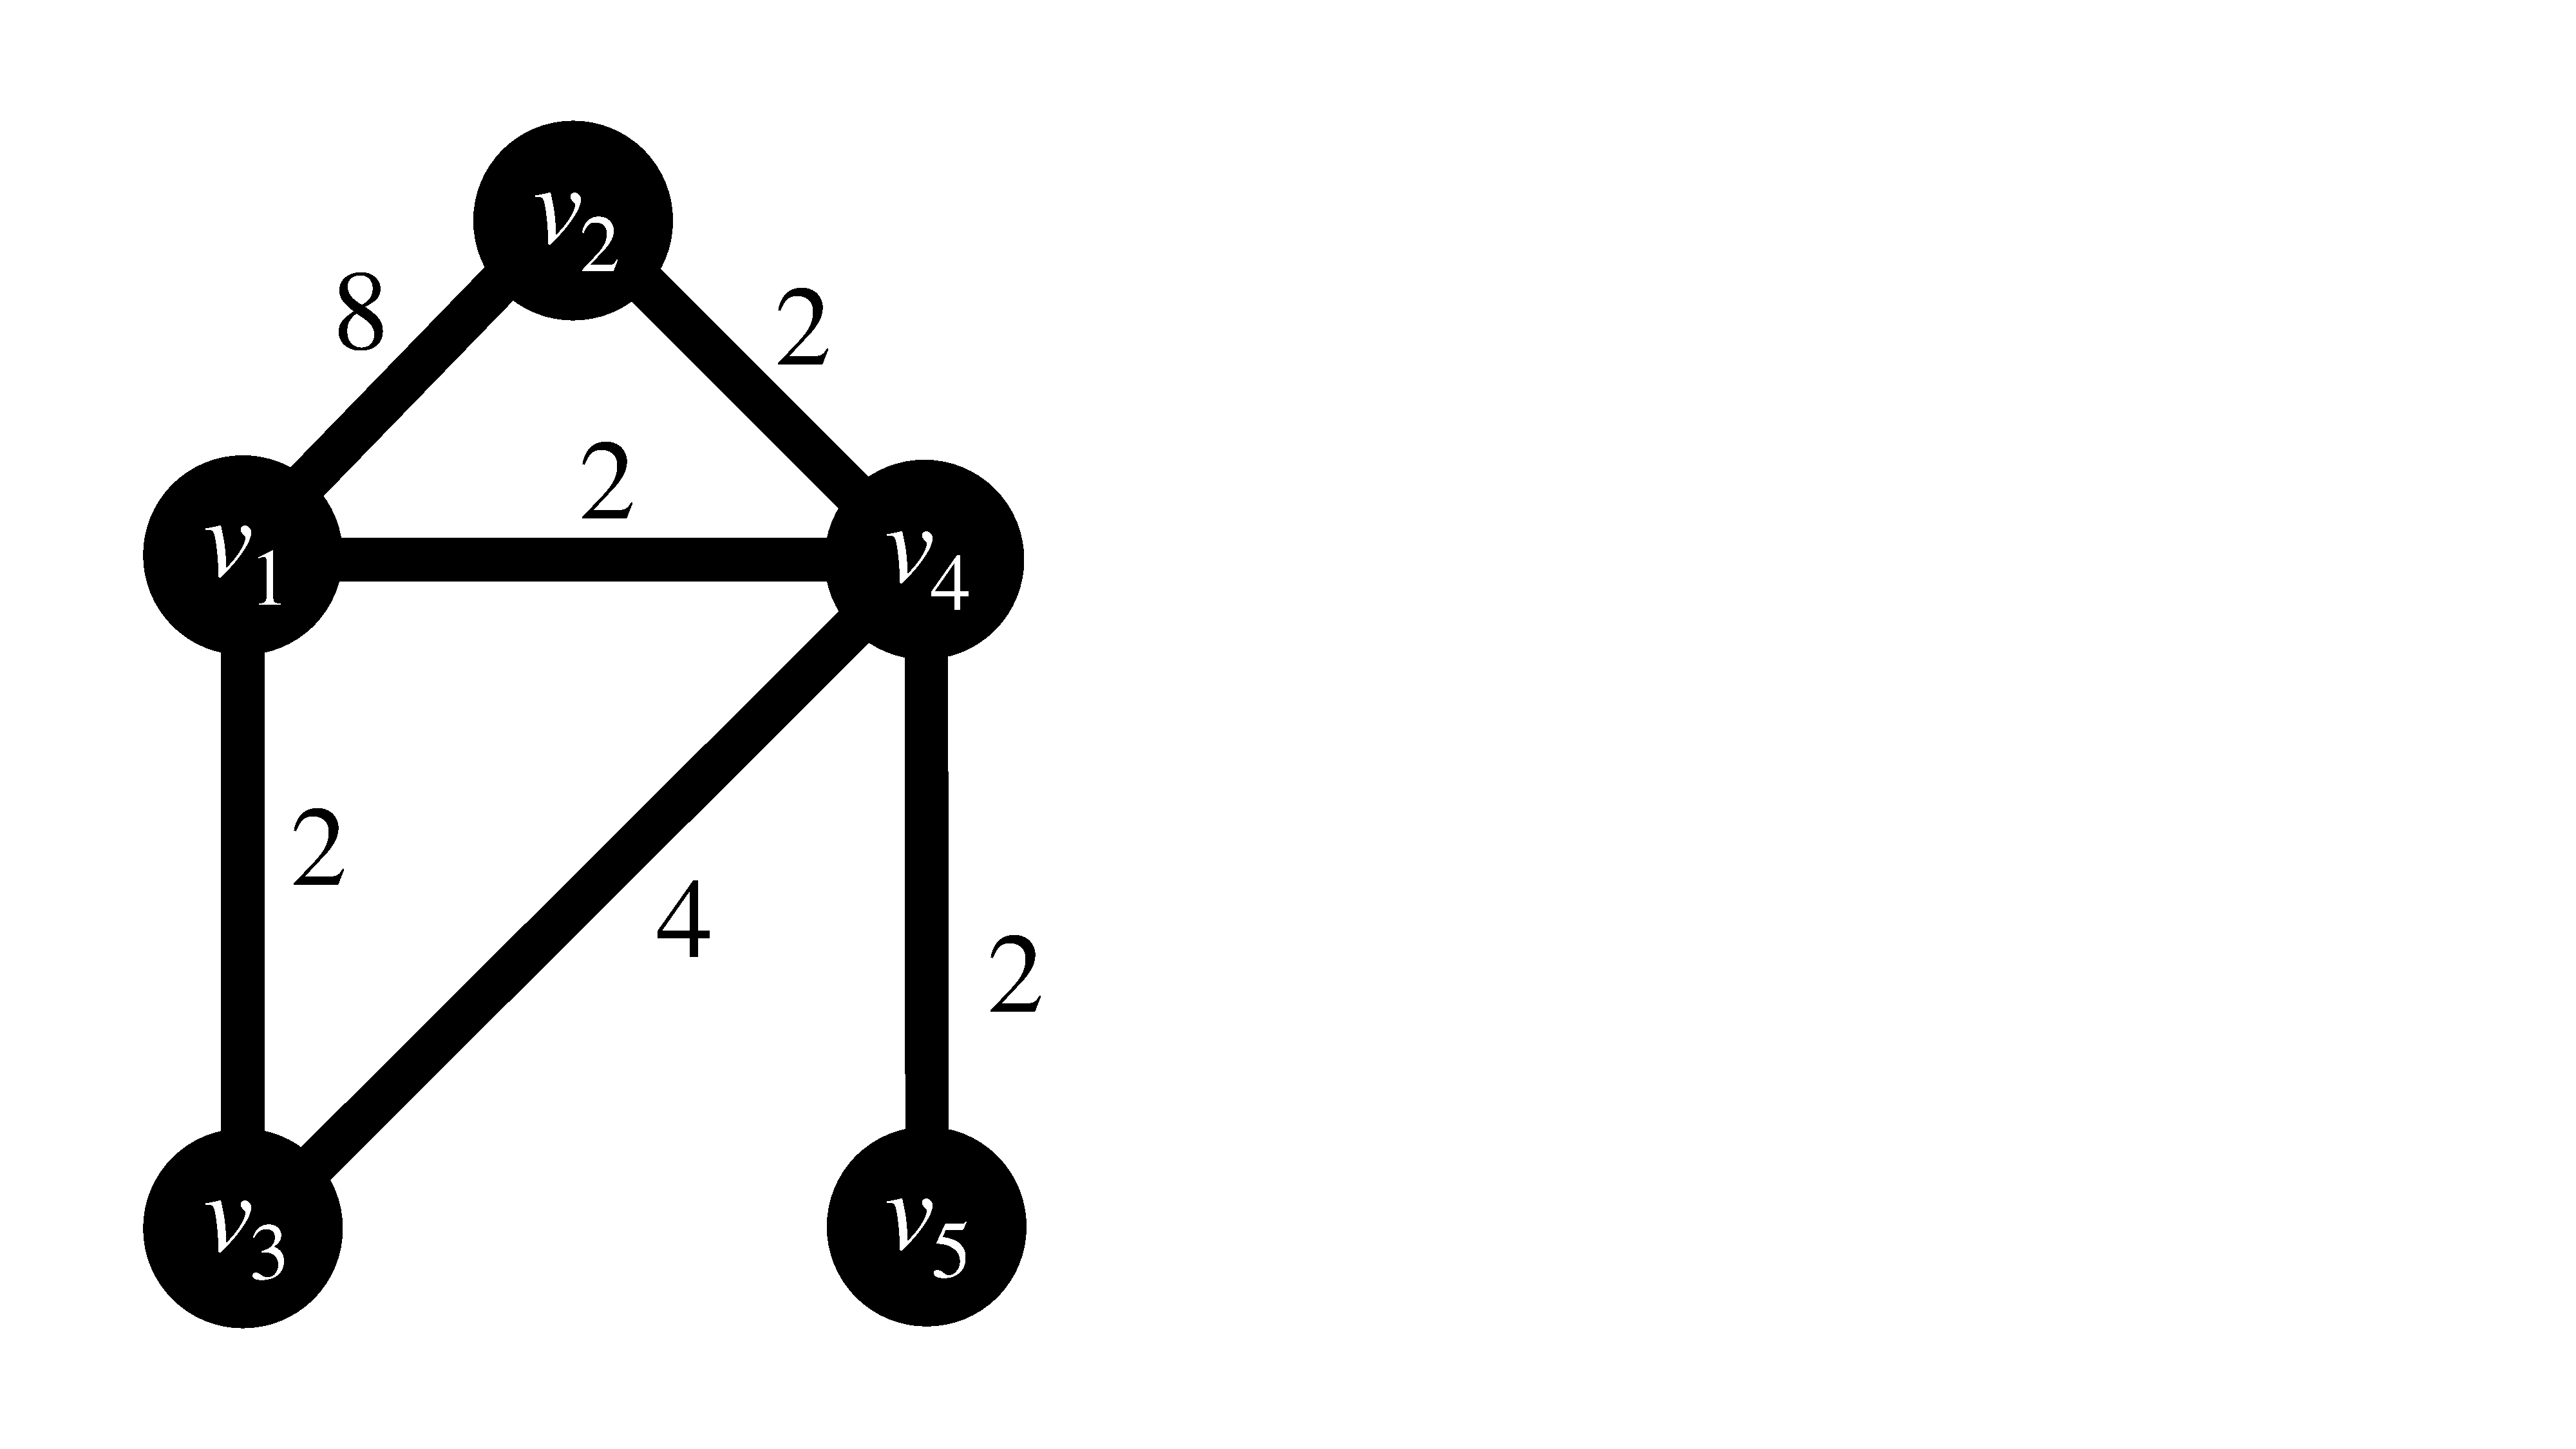
\includegraphics[width=\textwidth,trim=0mm 0mm 350mm 0mm, clip]{./figures/hac1.pdf}
        \caption{Input $G$.}\label{sfig:hac1}
    \end{subfigure} \hspace{3.5em} %\hfill
    \begin{subfigure}[b]{0.19\textwidth}
        \centering
        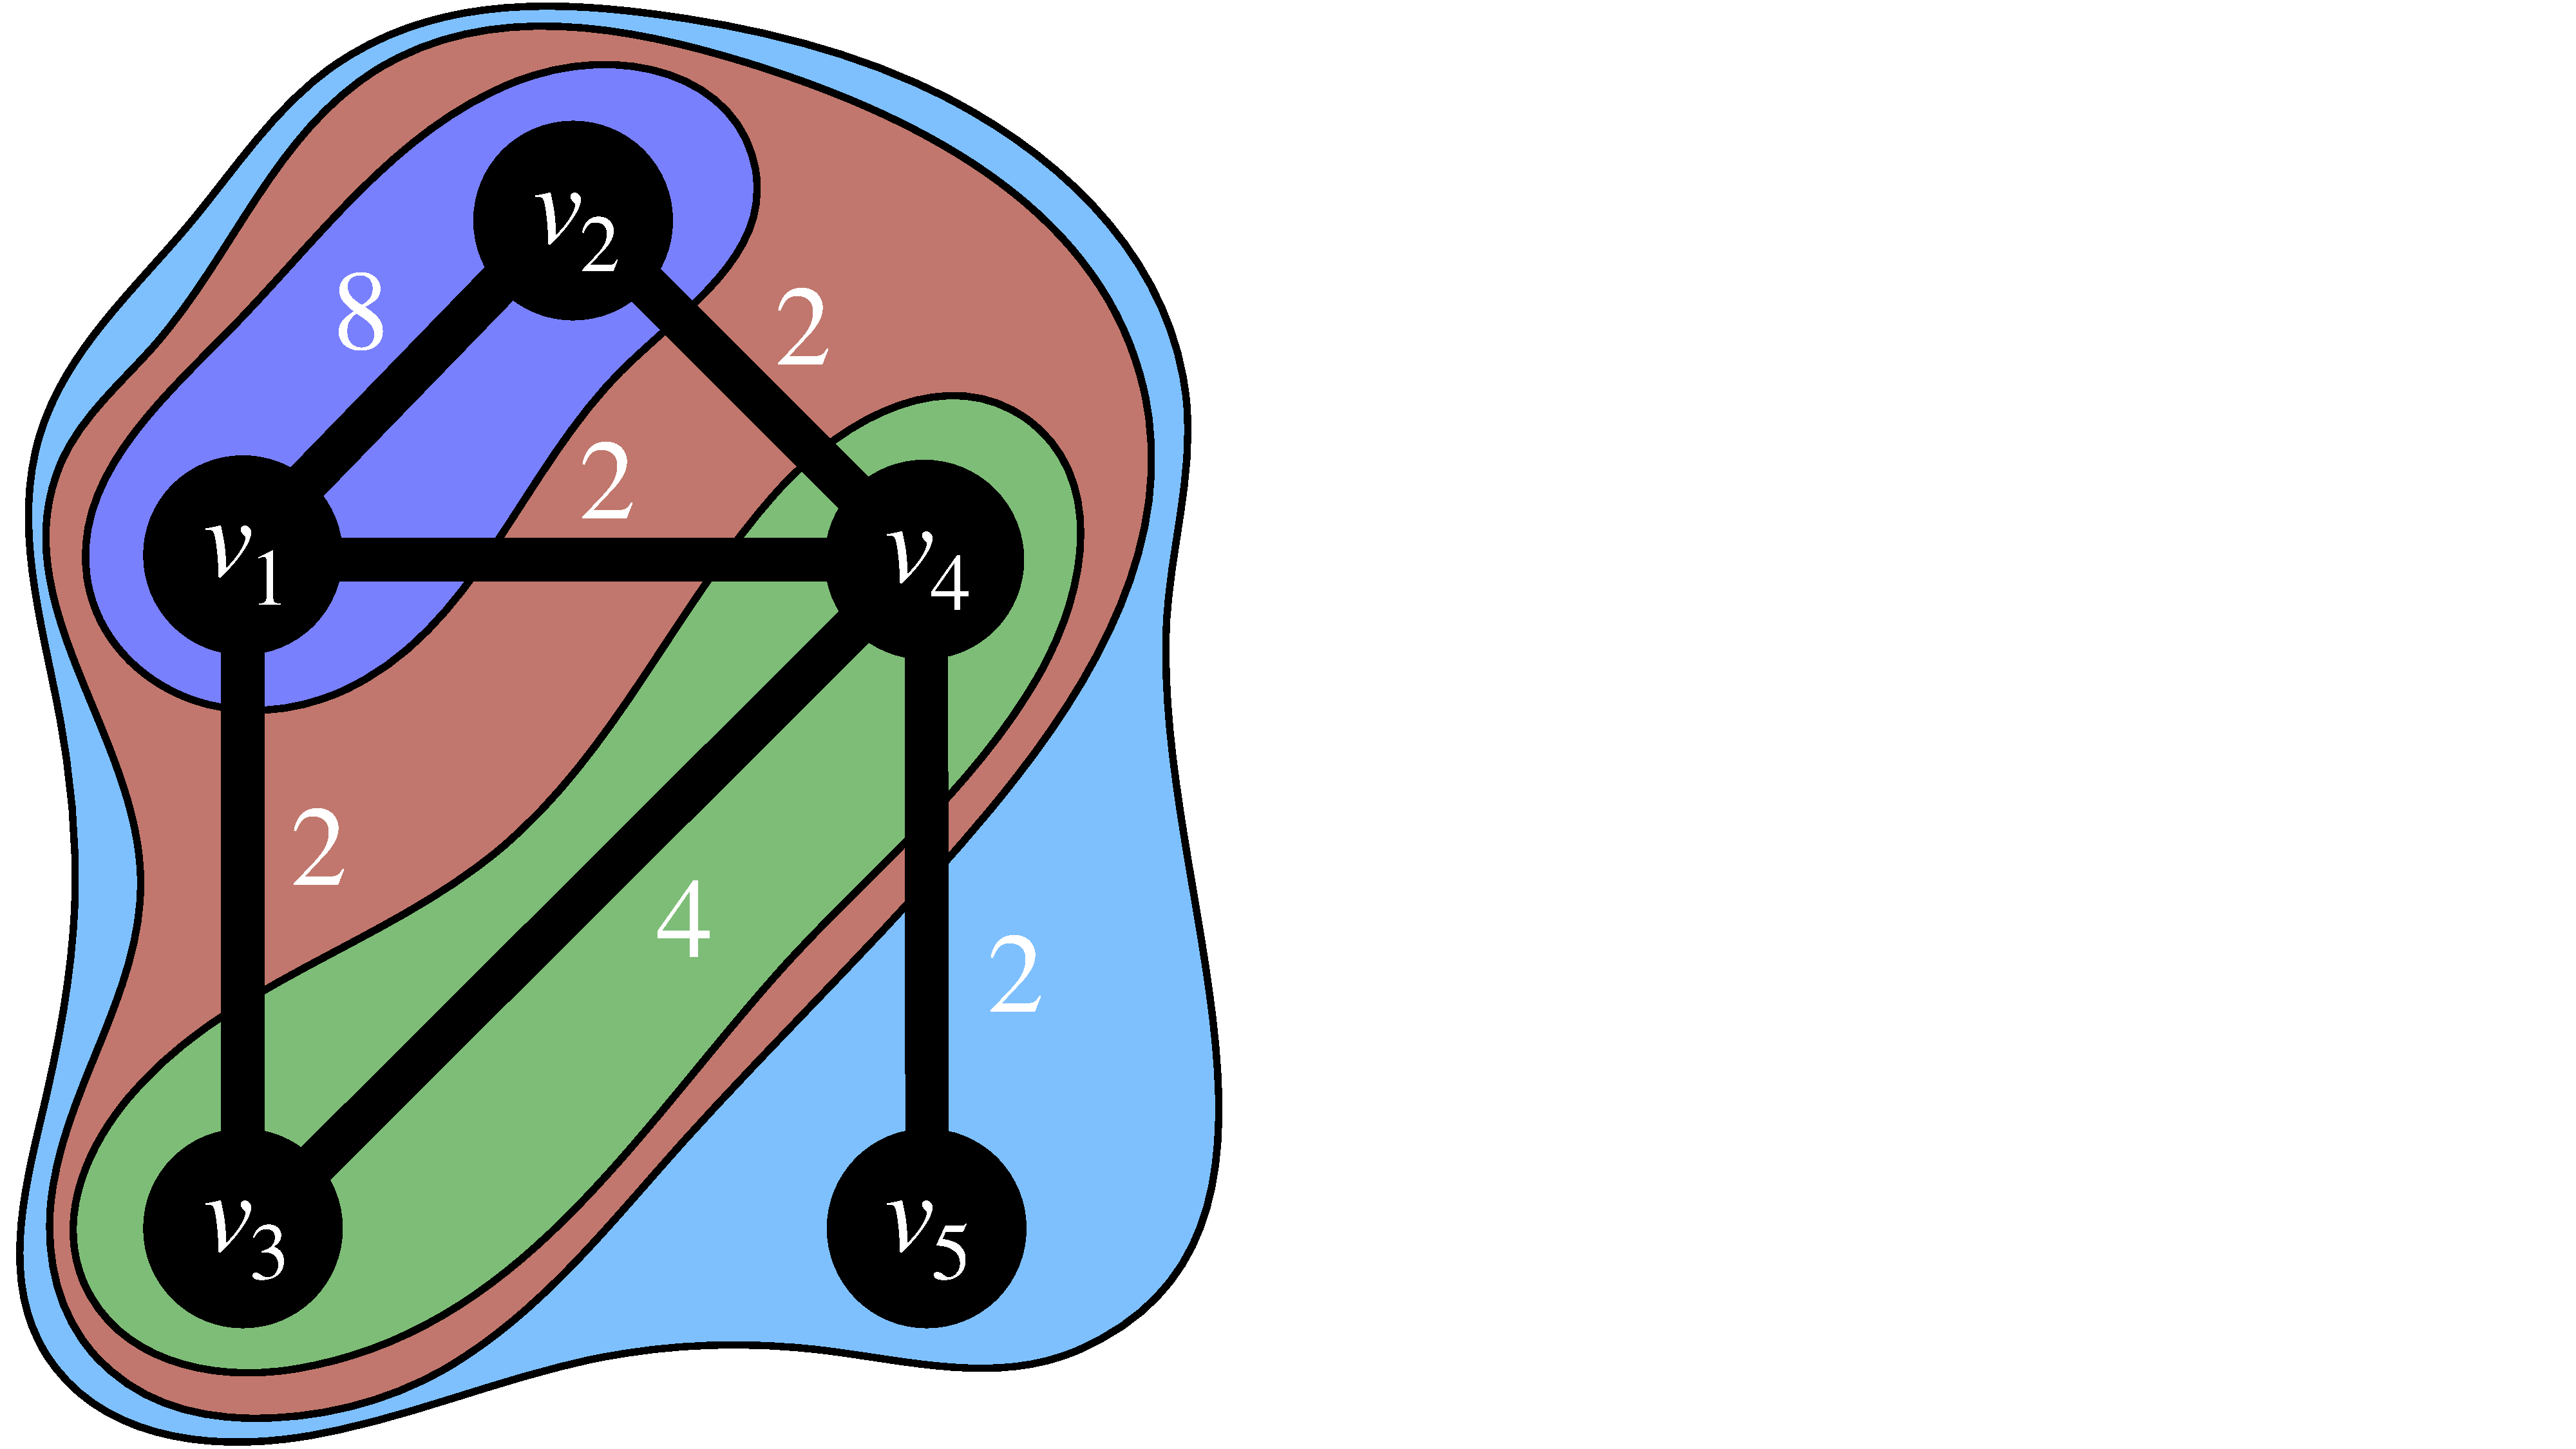
\includegraphics[width=\textwidth,trim=0mm 0mm 350mm 0mm, clip]{./figures/hac2.pdf}
        \caption{HAC Output.}\label{sfig:hac2}
    \end{subfigure}  \hspace{3.5em}%\hfill
    \begin{subfigure}[b]{0.19\textwidth}
        \centering
        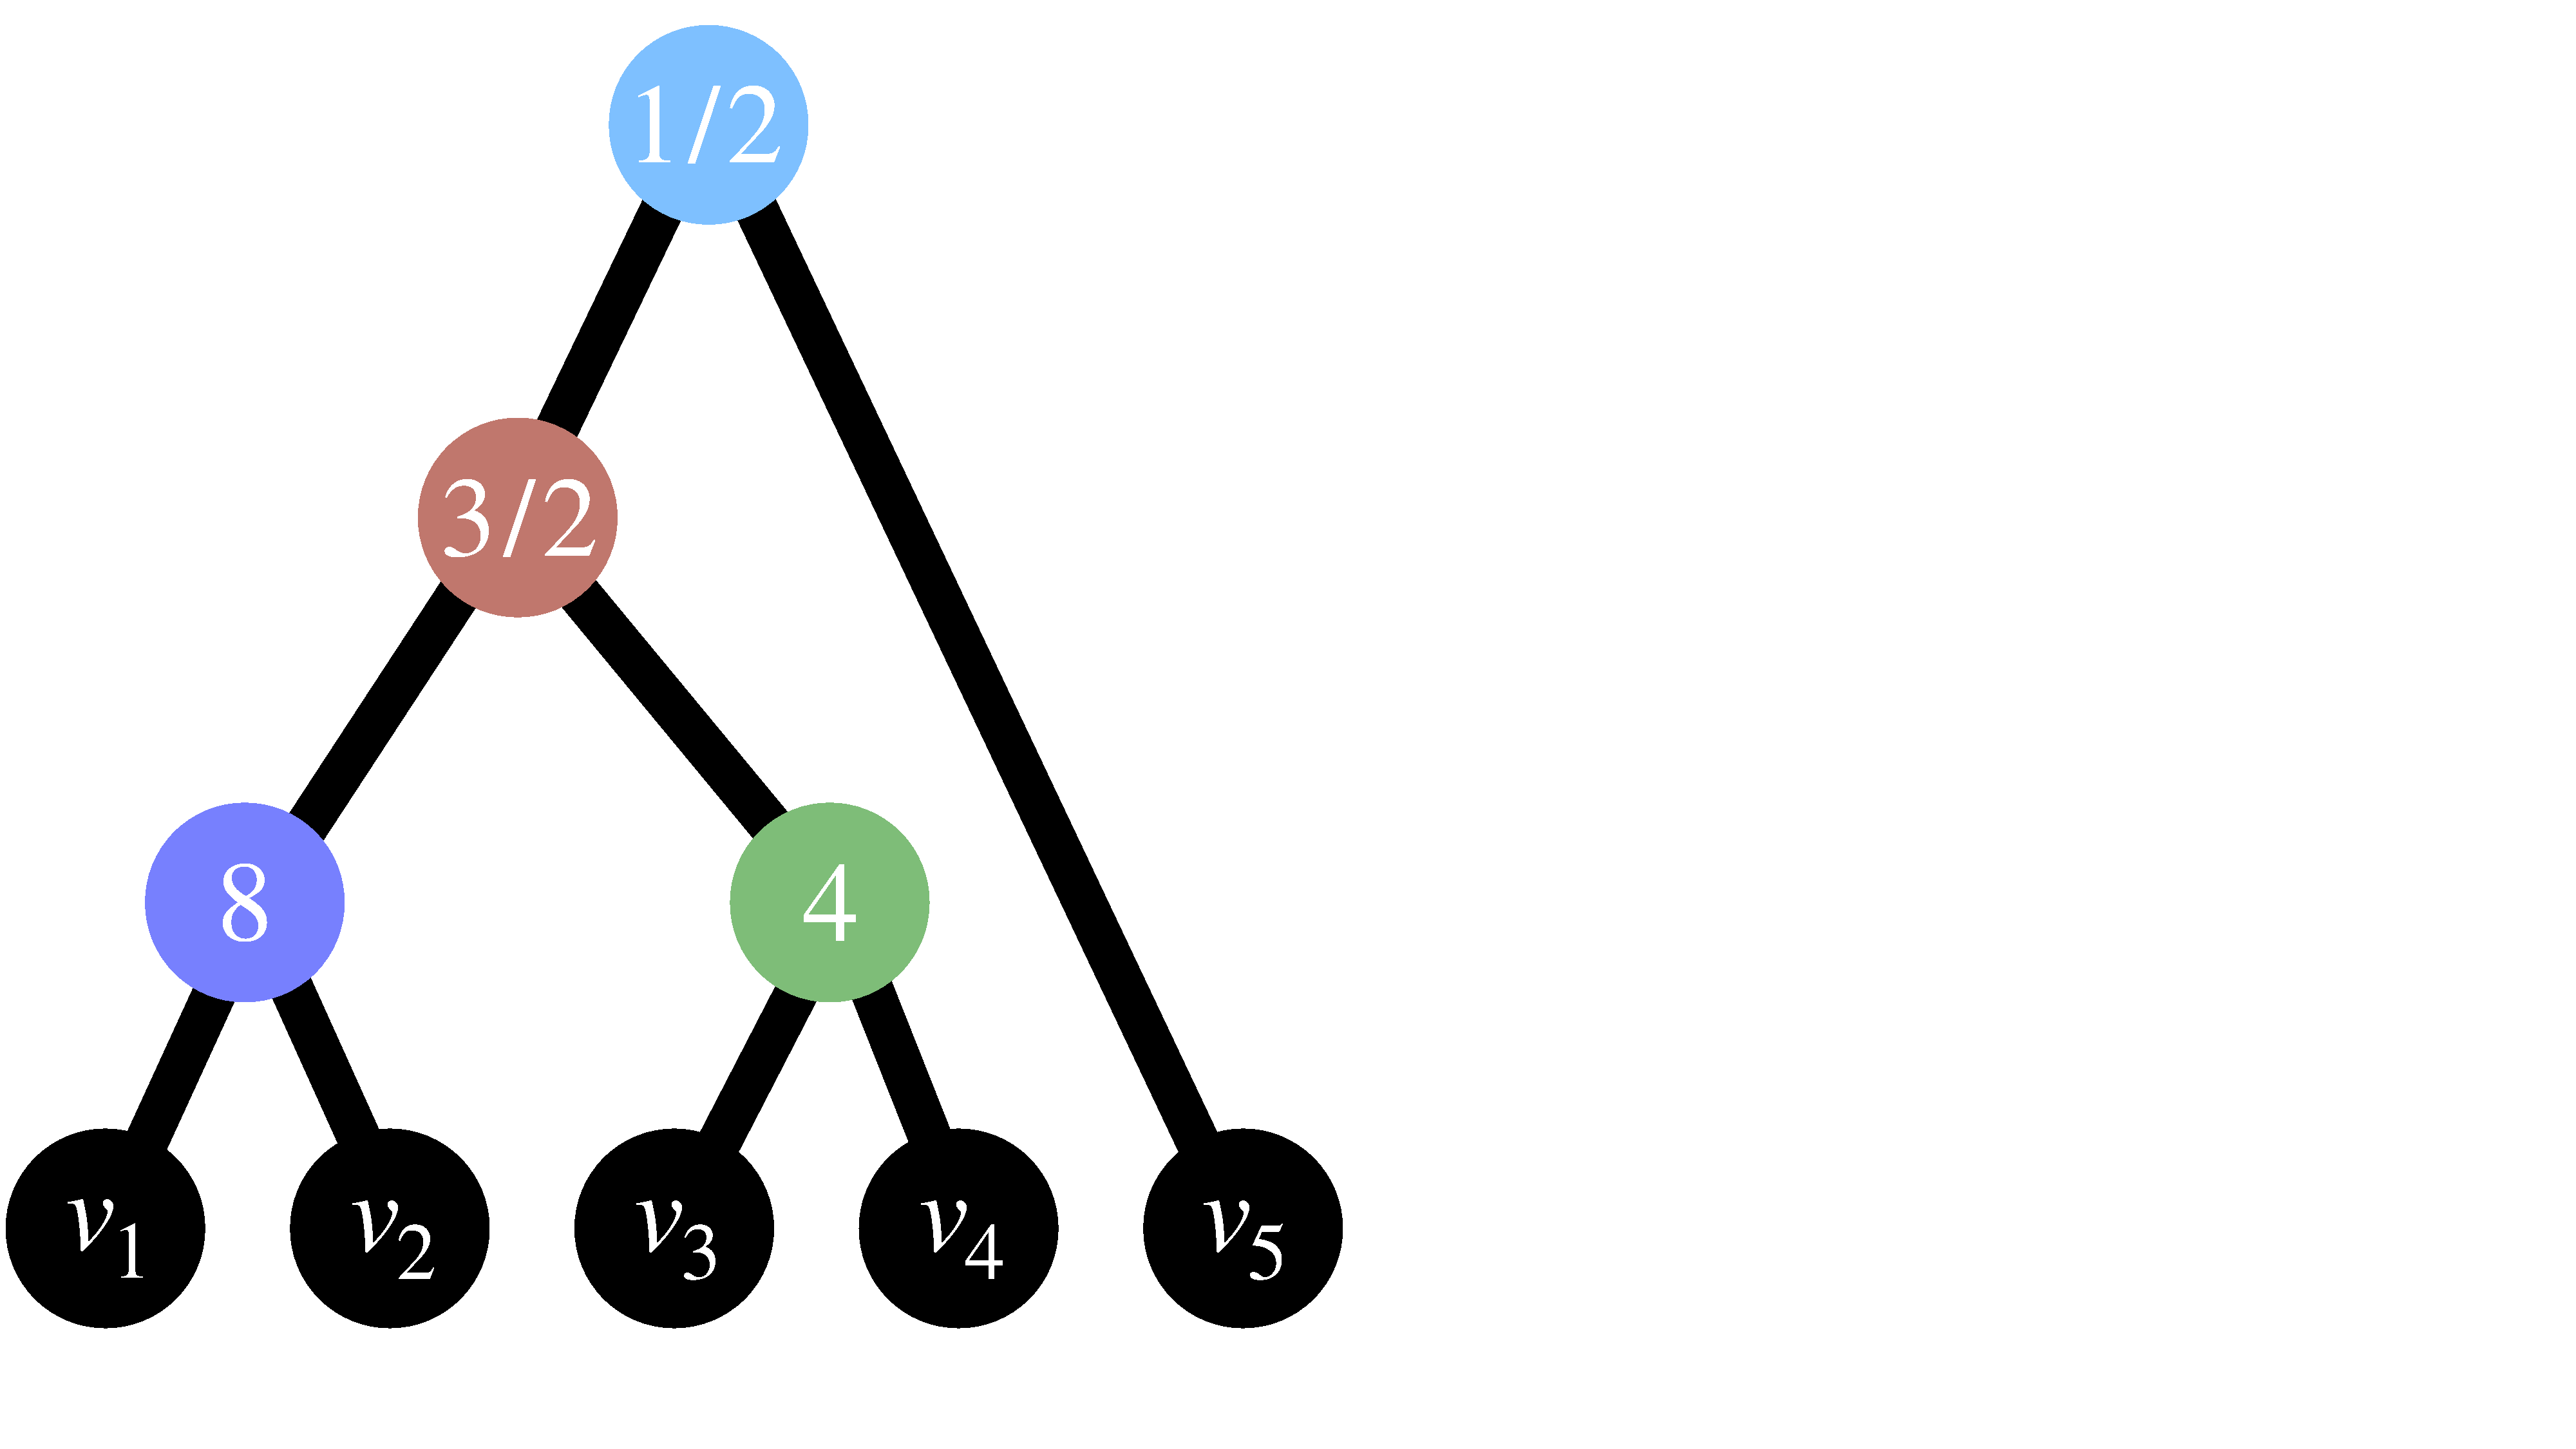
\includegraphics[width=\textwidth,trim=0mm 0mm 320mm 0mm, clip]{./figures/hac3.pdf}
        \caption{Dendrogram.}\label{sfig:hac3}
    \end{subfigure}   % \hfill
    \vspace{-0.5em}
    \caption{An example of average linkage HAC run on an input graph $G$. Edges labeled with weights. \ref{sfig:hac1} gives $G$. \ref{sfig:hac2} gives the cluster hierarchy output by HAC. \ref{sfig:hac3} gives the corresponding dendrogram with internal nodes labeled with the weight of their corresponding merge.} \label{fig:HAC}
\end{figure}

%Regarding (1), prior work \cite{dhulipala2021hierarchical} has shown that $\tilde{O}(n \sqrt{m})$ time algorithms are possible for average linkage HAC but a square root gap remains between this and the desired linear time. 

A natural algorithmic question then is how quickly can we solve average linkage HAC on $n$ node and $m$ edge graphs? 
Recent work has provided a partial answer to this basic question in sequential and parallel models of computation.
In particular, \cite{dhulipala2021hierarchical} showed that average linkage HAC can be solved in $\tilde{O}(n\sqrt{m})$ time, thus providing a sub-quadratic time algorithm for sufficiently sparse graphs.
A follow-up paper studied average linkage HAC in the parallel setting and showed that the problem is \PTime-complete and so likely does not admit \NC algorithms~\cite{dhulipala2022hierarchical}. 
However, the \PTime-completeness result of \cite{dhulipala2022hierarchical} holds for worst case graphs whereas typical applications of HAC are on highly structured graphs---namely those which are meant to capture relevant properties of an underlying metric---and so there is still hope for parallelizing average linkage HAC on more structured instances. 

In fact, such structured instances of average linkage HAC are known to admit much faster algorithms in the sequential setting: the sequential algorithm of \cite{dhulipala2021hierarchical} implies that if the input graph is planar (or, more generally, minor-free) average linkage HAC can be solved in time $\tilde{O}(m)$. 
More generally, if each graph obtained by contracting all clusters at each step of average linkage HAC has $O(1)$ arboricity\footnote{A graph has arboricity at most $\alpha$ if all of its edges can be covered by at most $\alpha$ trees.}, then it is possible to solve average linkage HAC in time $\tilde{O}(m)$; it follows that average linkage  HAC can be solved in sequential time $\tilde{O}(m)$ on trees or planar graphs.
In light of these improved sequential results for highly structured graphs, it becomes natural to hope for efficient parallel algorithms on structured graphs such as low arboricity graphs or, even, just trees.



%\enote{This sentence runs on} 

%\enote{Move background stuff up into questions}

%For (2), there has been significant recent effort in parallelizing HAC \cite{} but the best parallel algorithms for average linkage HAC require relaxing merging most similar clusters to merging approximately most similar clusters


%\knote{I think the questions may not be natural to the reader at this point. I'm wondering whether we could maybe summarize the SOTA here instead of after the questions: 1. In the sequential setting we have different bounds for exact and approximate HAC, but it's not clear whether we have to sacrifice exactness to get near linear time. 2. In the parallel setting, we know the problem is P-complete, but the examples are quite contrived}




\subsection{Our Contributions}
In this work, we continue the line of work which studied the computational complexity of different variants of HAC~\cite{greenlaw2008parallel, tsenghac, abboudhac, dhulipala2021hierarchical, dhulipala2022hierarchical} and perform a careful investigation into the complexity of average linkage HAC.
In particular, we study HAC on $n$ node and $m$ edge graphs and investigate whether
near-linear time algorithms, or more efficient parallel algorithms are possible, namely:
\begin{enumerate}
    \item \textbf{Near-Linear Time Algorithms:} Can we improve over the best known $\tilde{O}(n\sqrt{m})$ upper bound for average linkage HAC and obtain near-linear time sequential algorithms?
    
    \item \textbf{\NC Algorithms:} are there $\polylog(n)$ depth parallel algorithms for average linkage HAC with $\poly(n)$ work for highly structured instances, e.g., trees, or minor-closed graphs?
\end{enumerate}
%mature theory of the complexity
%In this work we provide a more complete picture of the complexity landscape of average linkage HAC. 
We give both new lower bounds which (conditionally) rule out near-linear time and \NC algorithms, and provide conditions under which these impossibility results can be bypassed.

First, we demonstrate that near-linear time algorithms are impossible under standard fine-grained complexity assumptions. 
%\enote{What is BMM? Maybe should be written out in the theorem}

\begin{restatable}{theorem}{mainLowerSeq}\label{thm:worklb}
    If average linkage HAC can be solved by a combinatorial algorithm in $O(n^{3/2-\epsilon})$ time for any $\epsilon > 0$, then the Combinatorial Boolean Matrix Multiplication (Combinatorial BMM) Conjecture is false.
\end{restatable}


Our reduction also implies a second (weaker) conditional lower bound that also holds for non-combinatorial algorithms (e.g., algebraic algorithms) based on the running time of matrix multiplication. 
In particular, for two $n \times n$ binary matrices, it is well known that matrix multiplication can be solved in time $O(n^{\omega})$ where $2 \leq \omega < 2.3716$~\cite{williams2024new}.
In this setting, we obtain the following result:

\begin{restatable}{theorem}{workmatmul}\label{cor:workmatmul}
If average linkage HAC can be solved by an algorithm in $O(n^{\omega/2-\epsilon})$ time for some $\epsilon > 0$, then boolean matrix multiplication can be solved in $O(n^{\omega - \epsilon'})$ time for some $\epsilon' > 0$.
\end{restatable}

\noindent 
Notably, Theorem~\ref{thm:worklb} shows that the prior running time of $\tilde{O}(n \sqrt{m})$ of \cite{dhulipala2021hierarchical} is {\em optimal} up to logarithmic factors under standard fine-grained complexity assumptions, at least for graphs consisting of $O(n)$ many edges.
We obtain this conditional lower bound by showing that a carefully constructed instance of HAC can be used to solve the triangle detection problem, which is sub-cubically equivalent to Boolean Matrix Multiplication~\cite{williams2010subcubic}.
We obtain a bound of (essentially) $\Omega(n^{3/2})$ since our reduction incurs a quadratic time and space blowup when transforming an input triangle detection instance to an instance of average linkage HAC.
%\enote{Say more about why this is hard / interesting}

We next turn to the parallel setting. 
Here, we show that HAC---\emph{even on trees}---is unlikely to admit efficient parallel algorithms. 
More formally, we show that average linkage HAC on low diameter trees is as hard as any problem in the complexity class Comparator Circuit (\CC) \cite{subramanian1989new, cook2014complexity}. 
It is believed that \CC is incomparable with \NC and that \CC-hardness is evidence that a problem is not parallelizable \cite{mayr1992complexity, cook2014complexity}.
\begin{restatable}{theorem}{mainLowerPar}\label{thm:mainLowerPar}
Average linkage HAC is \CC-hard, even on trees of diameter $4$.
\end{restatable}
\noindent We note that it is known that $\CC \subseteq \PTime$ and so the $\PTime$-hardness of \cite{dhulipala2022hierarchical} already suggests the impossibility of efficient parallel algorithms on \emph{general graphs}. 
However, our result suggests the impossibility of efficient parallel algorithms \emph{even on very simple graphs} (trees of diameter 4).
We obtain this result by reducing from the lexicographically first maximal matching (\lfm) problem and an intermediate problem which we call \am, which captures some of what makes HAC intrinsically difficult to parallelize.
%\enote{Say more about why this is hard / interesting}

On the positive side, we demonstrate that average linkage HAC on path graphs is in \NC, under the mild assumption that the aspect ratio is polynomial.
While the class of path graphs is restrictive, even on paths average linkage is highly non-trivial and naively running HAC requires resolving chains of $\Omega(n)$ sequential dependencies. For example, consider a path of vertices $(v_1, v_2, \ldots, v_n)$ where the edge $\{v_{i}, v_{i+1}\}$ has weight $1+i \cdot \epsilon$ for some small $\epsilon > 0$ and initially each vertex is in its own cluster. Initially, $v_n$'s most similar neighbor is $v_{n-1}$ and so $v_n$ would like to merge with $v_{n-1}$ but $v_{n-1}$'s most similar neighbor is $v_{n-2}$ and so on. Thus, whether or not $v_n$ gets to merge with $v_{n-1}$ depends on the merge behavior of $\Theta(n)$ other clusters and so it is not at all clear that \NC algorithms should be possible for this setting. Nonetheless, we show the following.
\begin{restatable}{theorem}{mainUpperPar}\label{thm:mainUpperPar}
    Average linkage HAC on paths is in \NC. In particular, there is an algorithm for average linkage HAC that runs in $O(\log^2 n \log\log n)$ depth with $O(n\log n\log\log n)$ work.
%    \enote{Maybe say something about work being essentially linear?}
\end{restatable}
\noindent  The above algorithm leverages the fact that in average linkage HAC the maximum edge similarity monotonically decreases. In particular, it works in $O(\log n)$ phases where each phase consists of merges of equal similarity up to constants. The goal then becomes to efficiently perform merges until every edge is no longer within a constant of the starting maximum similarity of the phase. The starting point of the algorithm is to observe that $\Omega(n)$ sequential dependencies of clusters of equal size can be resolved efficiently in parallel in a phase by noting that in this phase only the odd-indexed edges merge in the chain. Thus, each edge can decide if it is odd-indexed in parallel by, e.g., using $\mathsf{prefix\text{-}sum}$, which is well known to be solvable in linear work in \NC.

For chains with clusters of general weights, we decompose dependency chains into short ($(O(\log n)$-length) subchains where resolving dependencies within the subchain must be done sequentially but in the current phase each subchain's merge behavior only depends on whether or not its closest neighboring subchains merges into it or not. Thus, each subchain can compute its merge behavior for these two cases and then, similar to the equal weights setting, we propagate merge behavior across subchains efficiently in parallel.

To complement our sequential lower bound with a positive result, we demonstrate that it is possible to achieve near-linear running time, provided the dendrogram has low height. Thus, if the output dendrogram is a relatively balanced tree, then near-linear time algorithms are possible.
%\knote{Reorder theorems?}
%\enote{Say more about why this is reasonable; would be nice if we could say in practice the dendrogram depth is low.}
%\hnote{We could report stats about dendrom height of HAC for {\it all} datasets used in prior HAC papers, and then mention some anecdotal information from internal datasets.}
\begin{restatable}{theorem}{mainUpperSec}\label{thm:mainUpperSeq}
    There is an implementation of the nearest-neighbor chain algorithm for average linkage HAC that runs in $O(m \cdot h \log n)$ time where $h$ is the height of the output dendrogram.
\end{restatable}
\noindent The above result is in fact obtained by a relatively simple (but to the best of our knowledge, new) analysis of {\em existing} classic HAC algorithms.
In particular, we show that the nearest-neighbor chain~\cite{benzecri, juan} and heap-based algorithms~\cite{irbook} for HAC, which were developed over 40 years ago achieve this bound. 
%Due to space constraints, we prove Theorem~\ref{thm:mainUpperSeq} in Appendix~\ref{sec:workupperbound}.



% \begin{itemize}
% \item HAC is included in many scikit-learn, scipy, etc
% \item HAC is being applied to gigantic datasets so makes sense to care about parallel and near-linear-time algs
% \item HAC has been studied from theory perspective by many of recent (of our) papers
% \hnote{Maybe a separate item: there has been a lot of effort for parallelizing graph algorithms recently, though our understanding of the parallel lower bounds is very limited.}
% \end{itemize}

\section{Preliminaries}\label{sec:prelims}
The input to the HAC algorithm is an undirected weighted graph $G=(V, E, w)$, where $w : V \times V \rightarrow \mathbb{R}_+ \cup \{0\}$ is a function assigning nonnegative weights to the edges.
For convenience we assume $w(x, y) = 0$ when $xy \not\in E$.
%\hnote{Shall we say that this is the sum of the weights of all parallel edges? Or shall we address this at the definition of merging below?}
The vanilla version of average linkage HAC is given as \cref{alg:staticgraph}.
It starts by putting each vertex in a cluster of size $1$ and then repeats the following step.
While there is a pair of clusters of positive similarity, find two most similar clusters and merge them together, that is, replace them by their union.
The similarity between two clusters is the total edge weight between them divided by the product of the cluster sizes.
We refer to this version as the \emph{static graph} version, since the graph is not changed throughout the run of the algorithm.

Throughout the paper we usually work with a different (equivalent) way of presenting the same algorithm which is given as \cref{alg:contractions} (e.g., \Cref{alg:nnchain,alg:heapbased}).
In this version we maintain a graph $G$ whose vertices are clusters.
The \emph{size} of the vertex is the size of the cluster it represents.
The \emph{normalized} weight of an edge $xy$ in $G$ is $w(x,y)$ divided by the product of the sizes of $x$ and $y$.
%In what follows, when we discuss the {\em weight} of an edge between two clusters, we mean the normalized edge weight (i.e., the average linkage weight) unless mentioned otherwise.

Whenever two clusters merge, their corresponding vertices are merged into one, i.e., the edge between them is contracted and the size of the new vertex is the sum of the sizes of the vertices that merged.
In the following we sometimes say that a vertex $x$ merges into vertex $y$.
In this case we simply assume that the name of the resulting vertex is $y$ and the size of $y$ is increased by the size of $x$. See \Cref{fig:HACMerge}.

\begin{figure}[h]
    \centering
    \vspace{-0.5em}
    \begin{subfigure}[b]{0.19\textwidth}
        \centering
        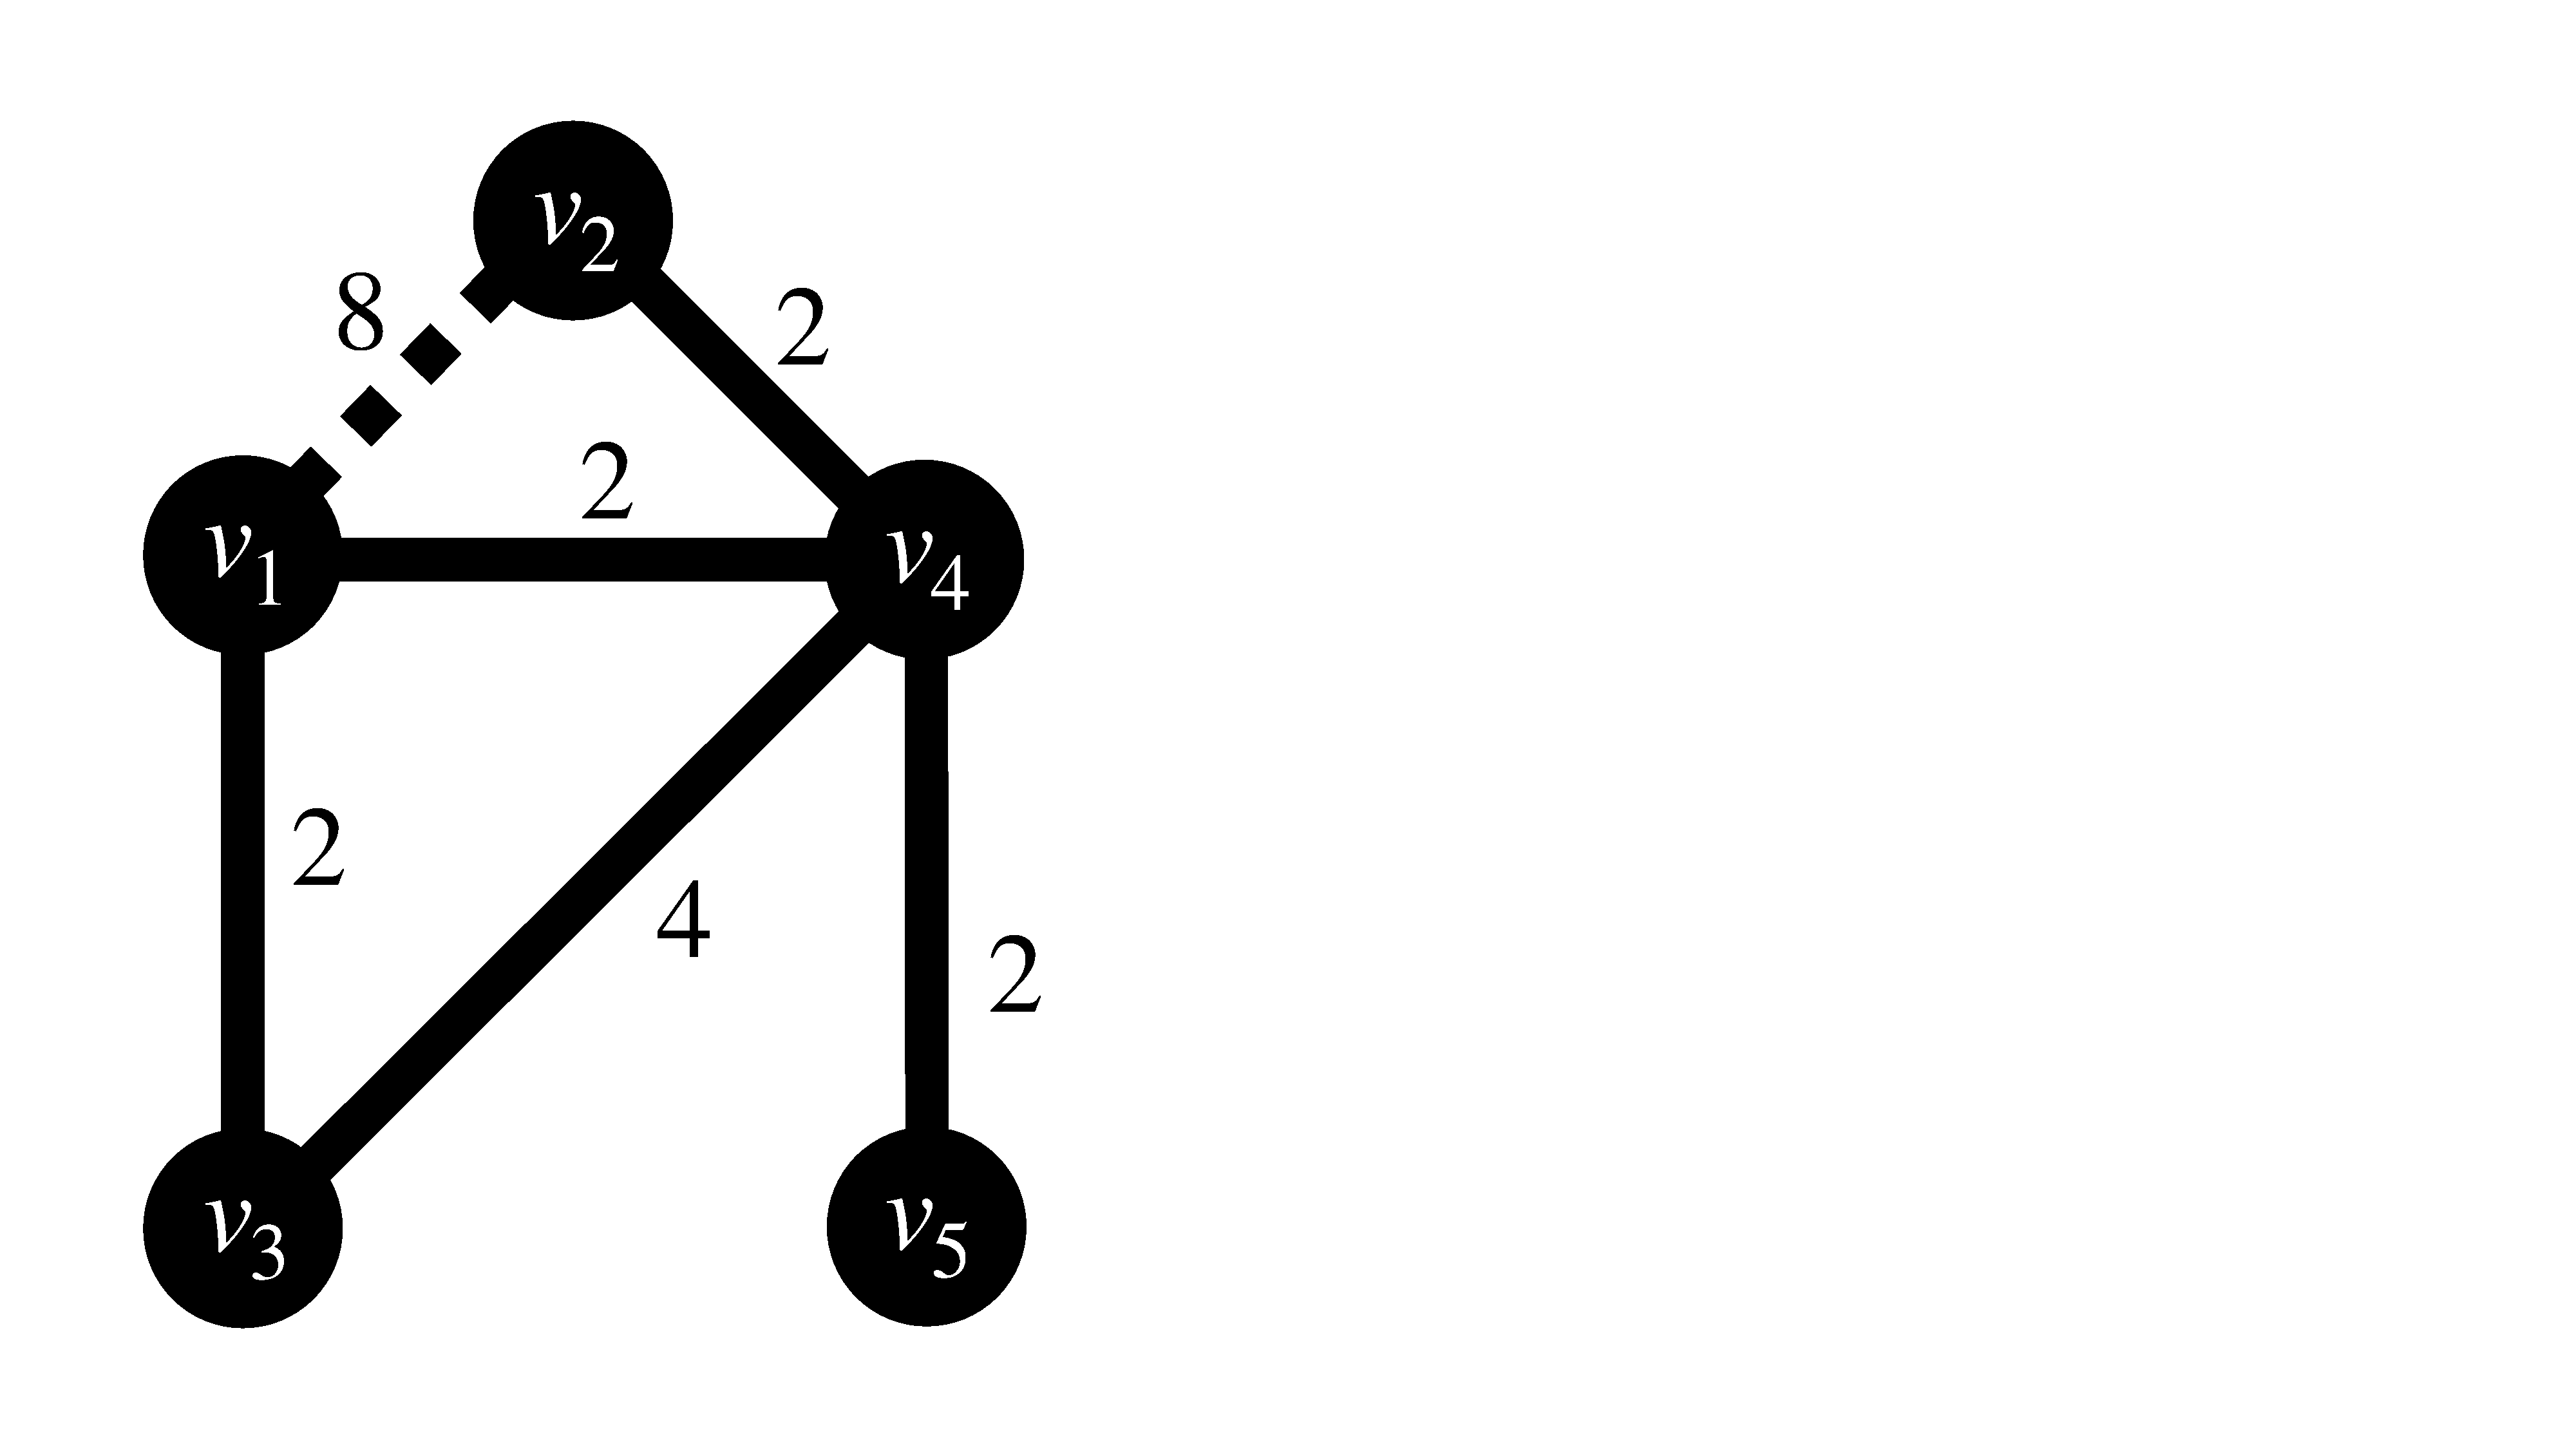
\includegraphics[width=\textwidth,trim=0mm 0mm 350mm 0mm, clip]{./figures/hacMerge1.pdf}
        \caption{Input $G$.}\label{sfig:hacMerge1}
    \end{subfigure} \hfill
    \begin{subfigure}[b]{0.19\textwidth}
        \centering
        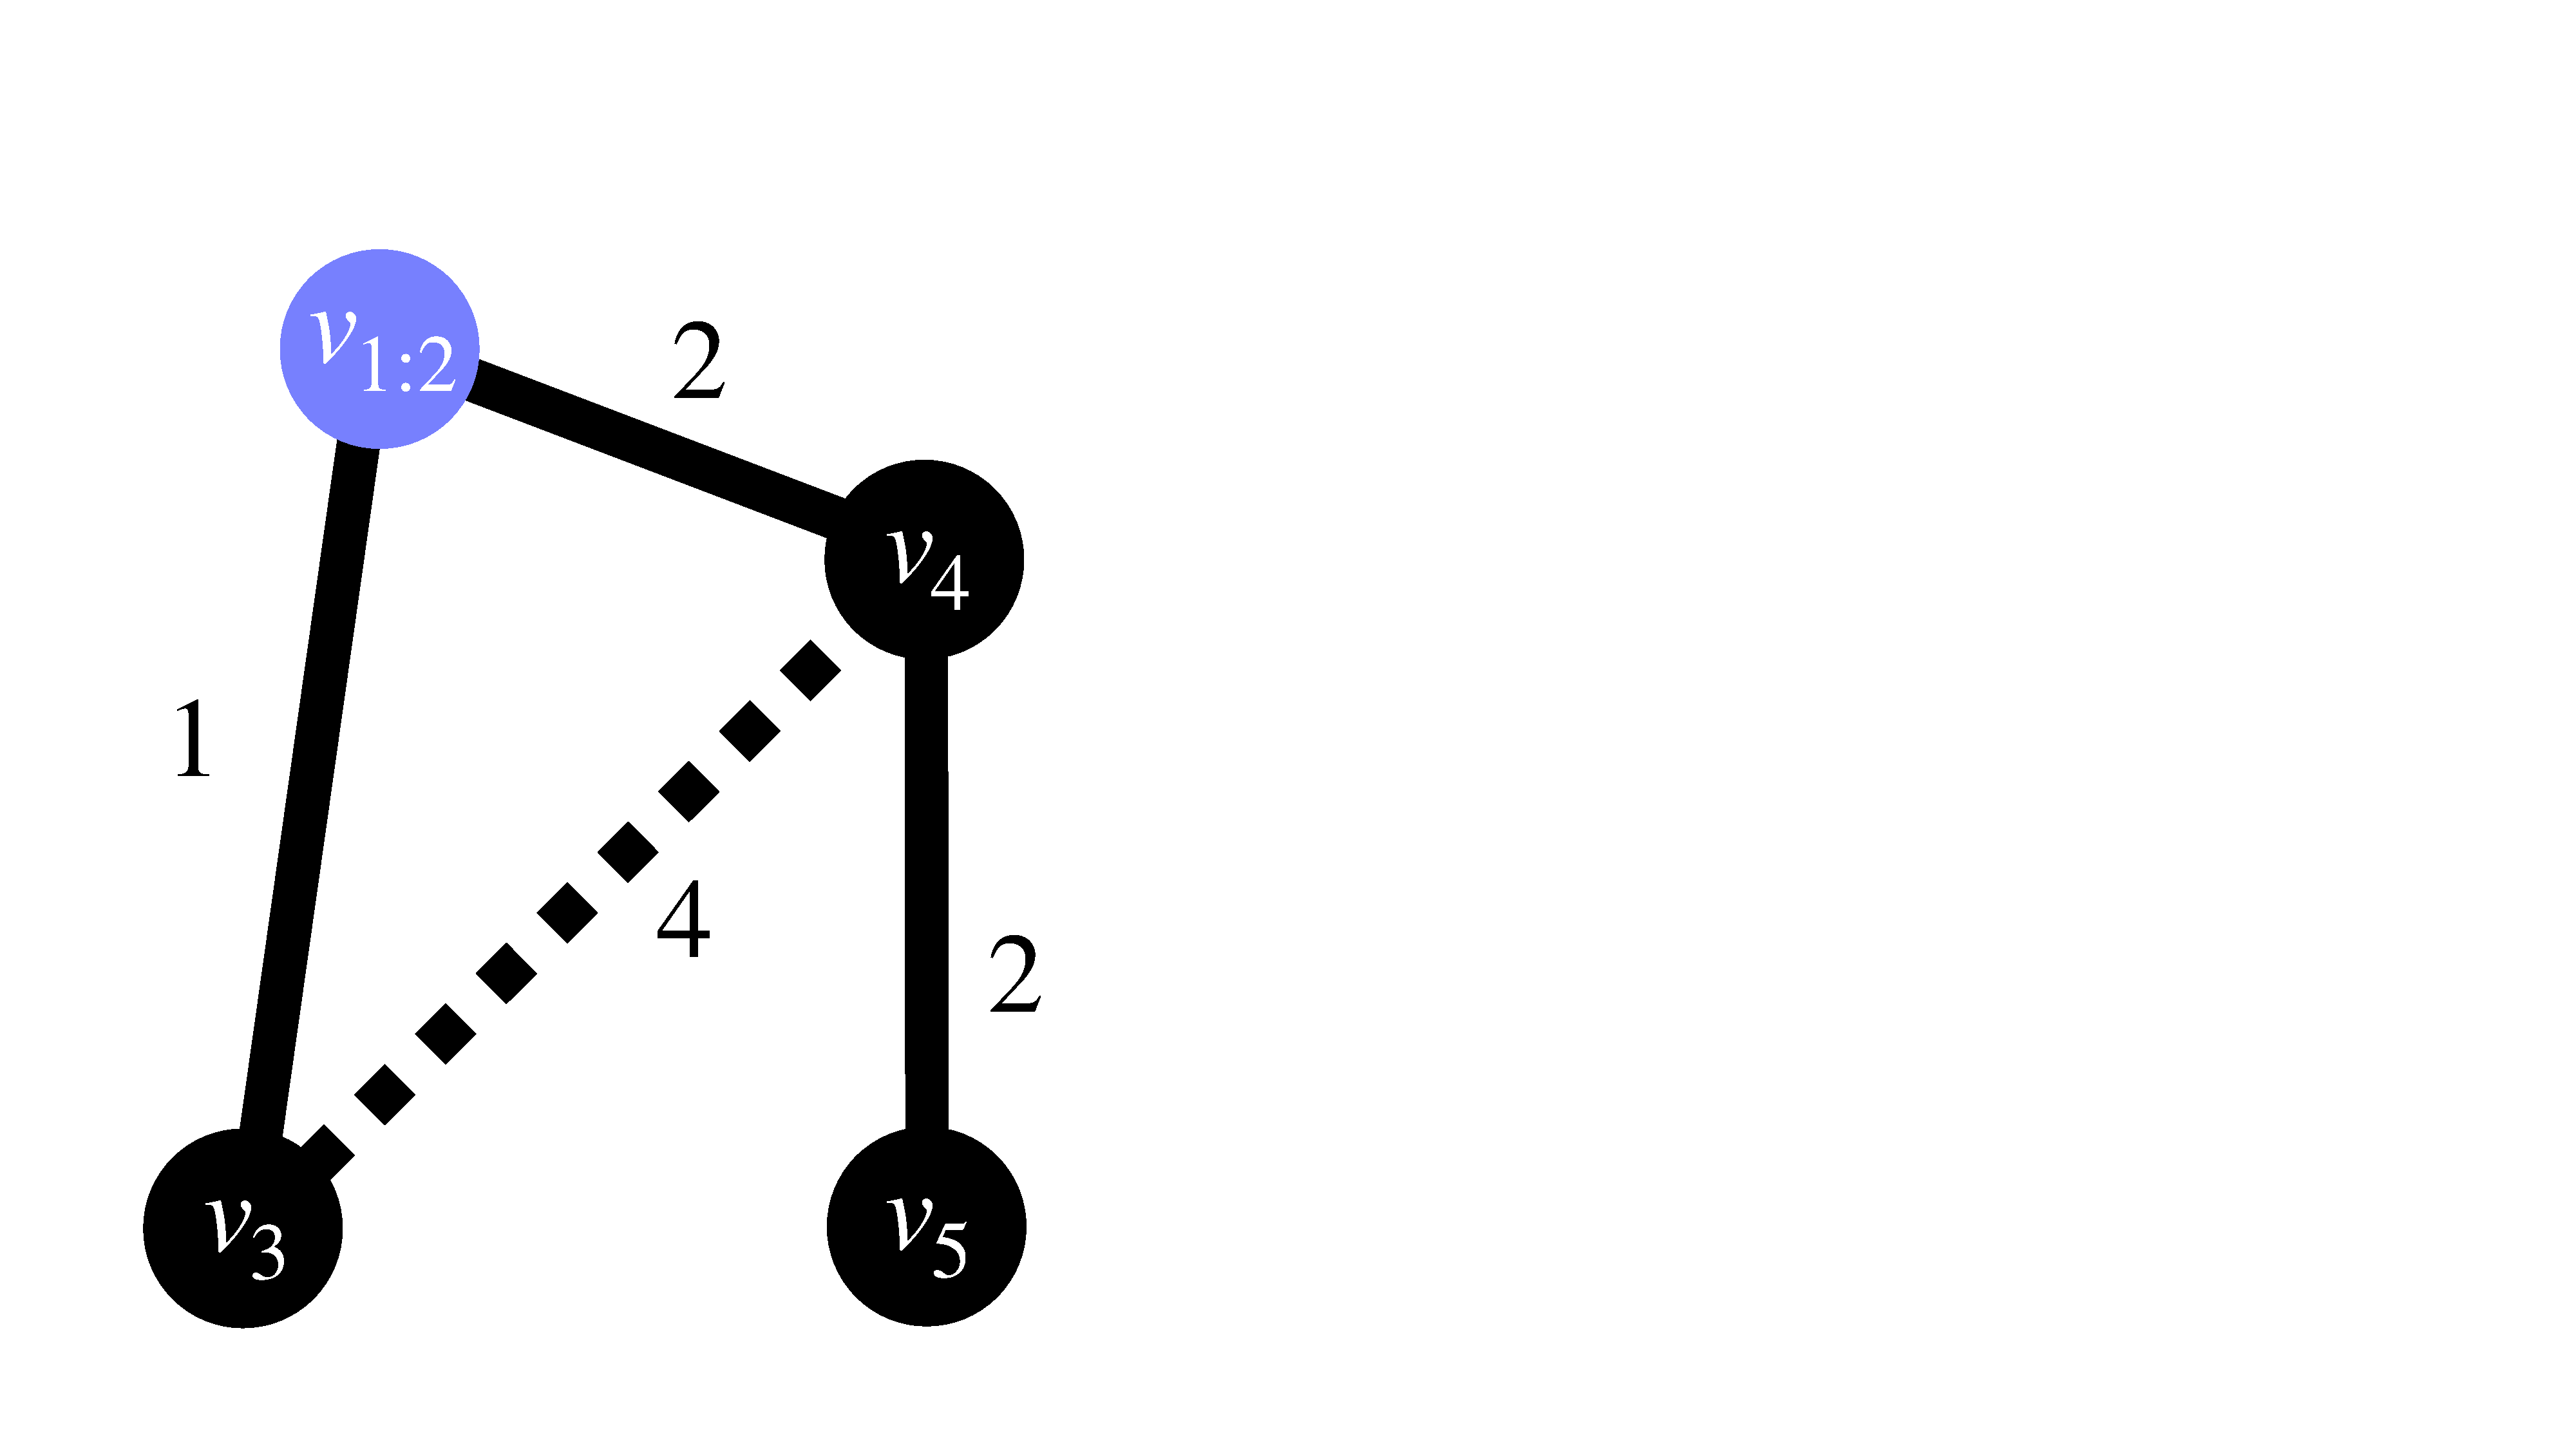
\includegraphics[width=\textwidth,trim=0mm 0mm 350mm 0mm, clip]{./figures/hacMerge2.pdf}
        \caption{1 merge.}\label{sfig:hacMerge2}
    \end{subfigure}  \hfill
    \begin{subfigure}[b]{0.19\textwidth}
        \centering
        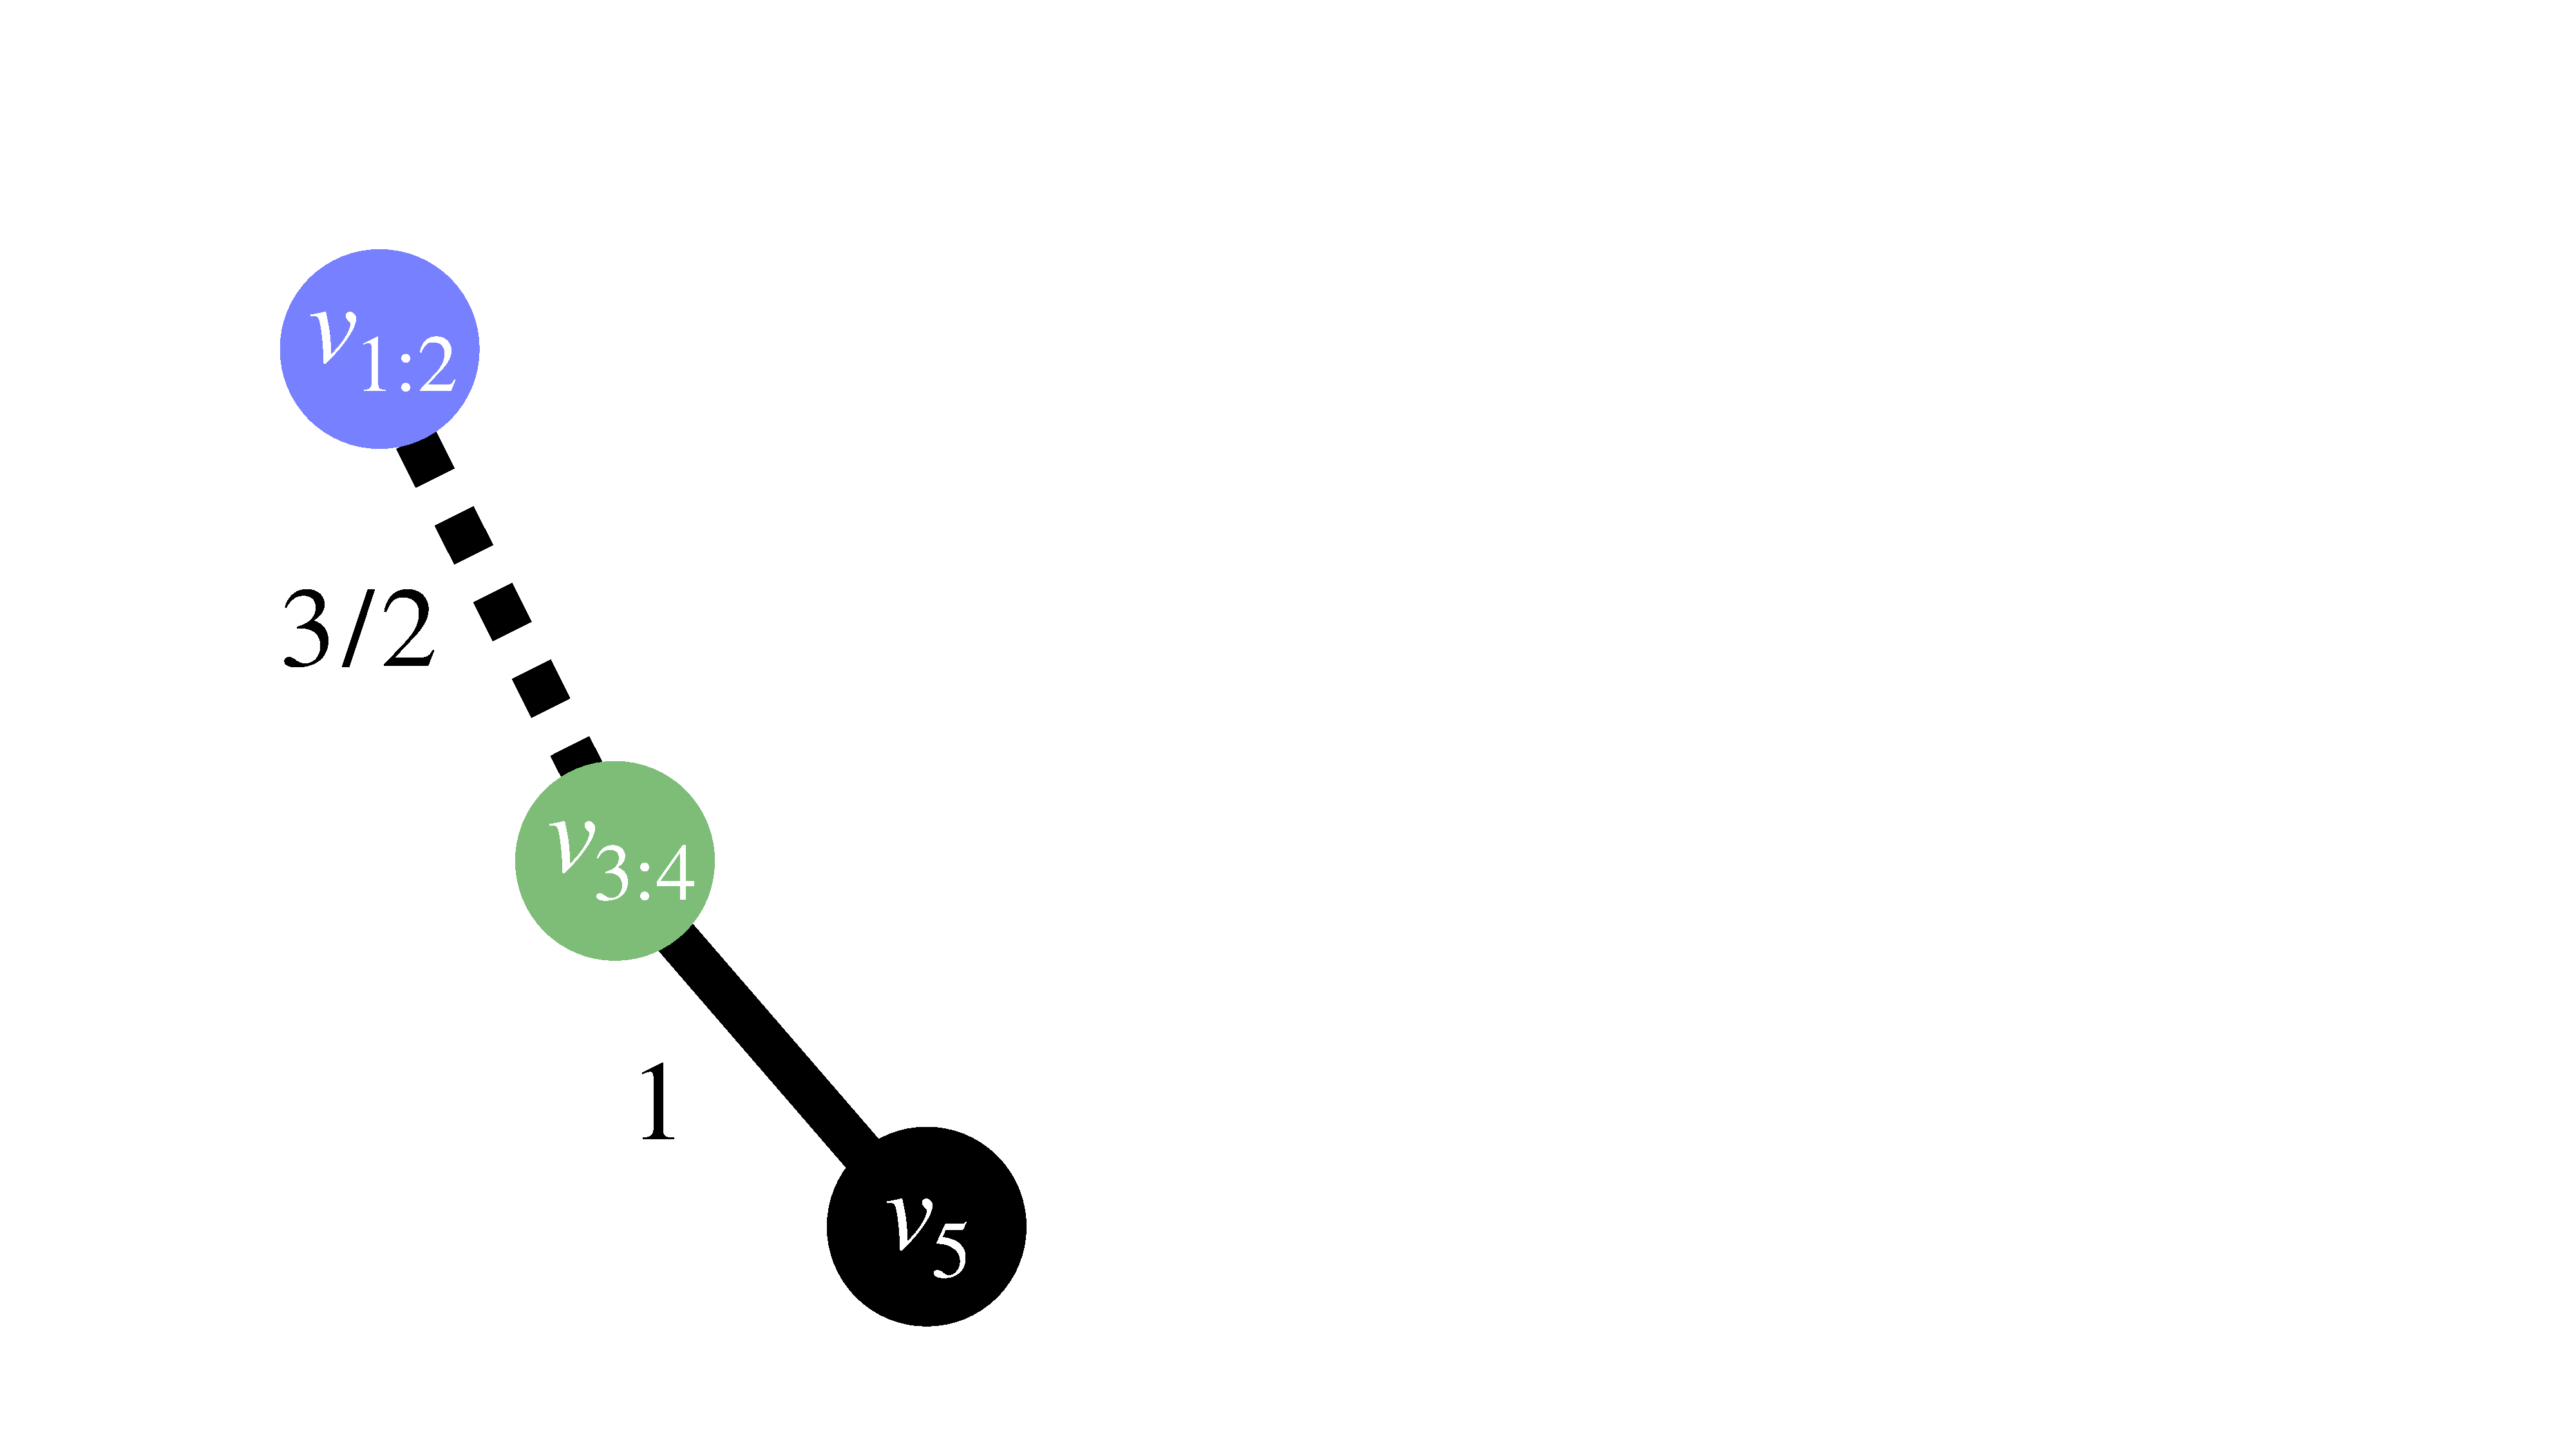
\includegraphics[width=\textwidth,trim=0mm 0mm 320mm 0mm, clip]{./figures/hacMerge3.pdf}
        \caption{2 merges.}\label{sfig:hacMerge3}
    \end{subfigure}   \hfill
        \begin{subfigure}[b]{0.19\textwidth}
        \centering
        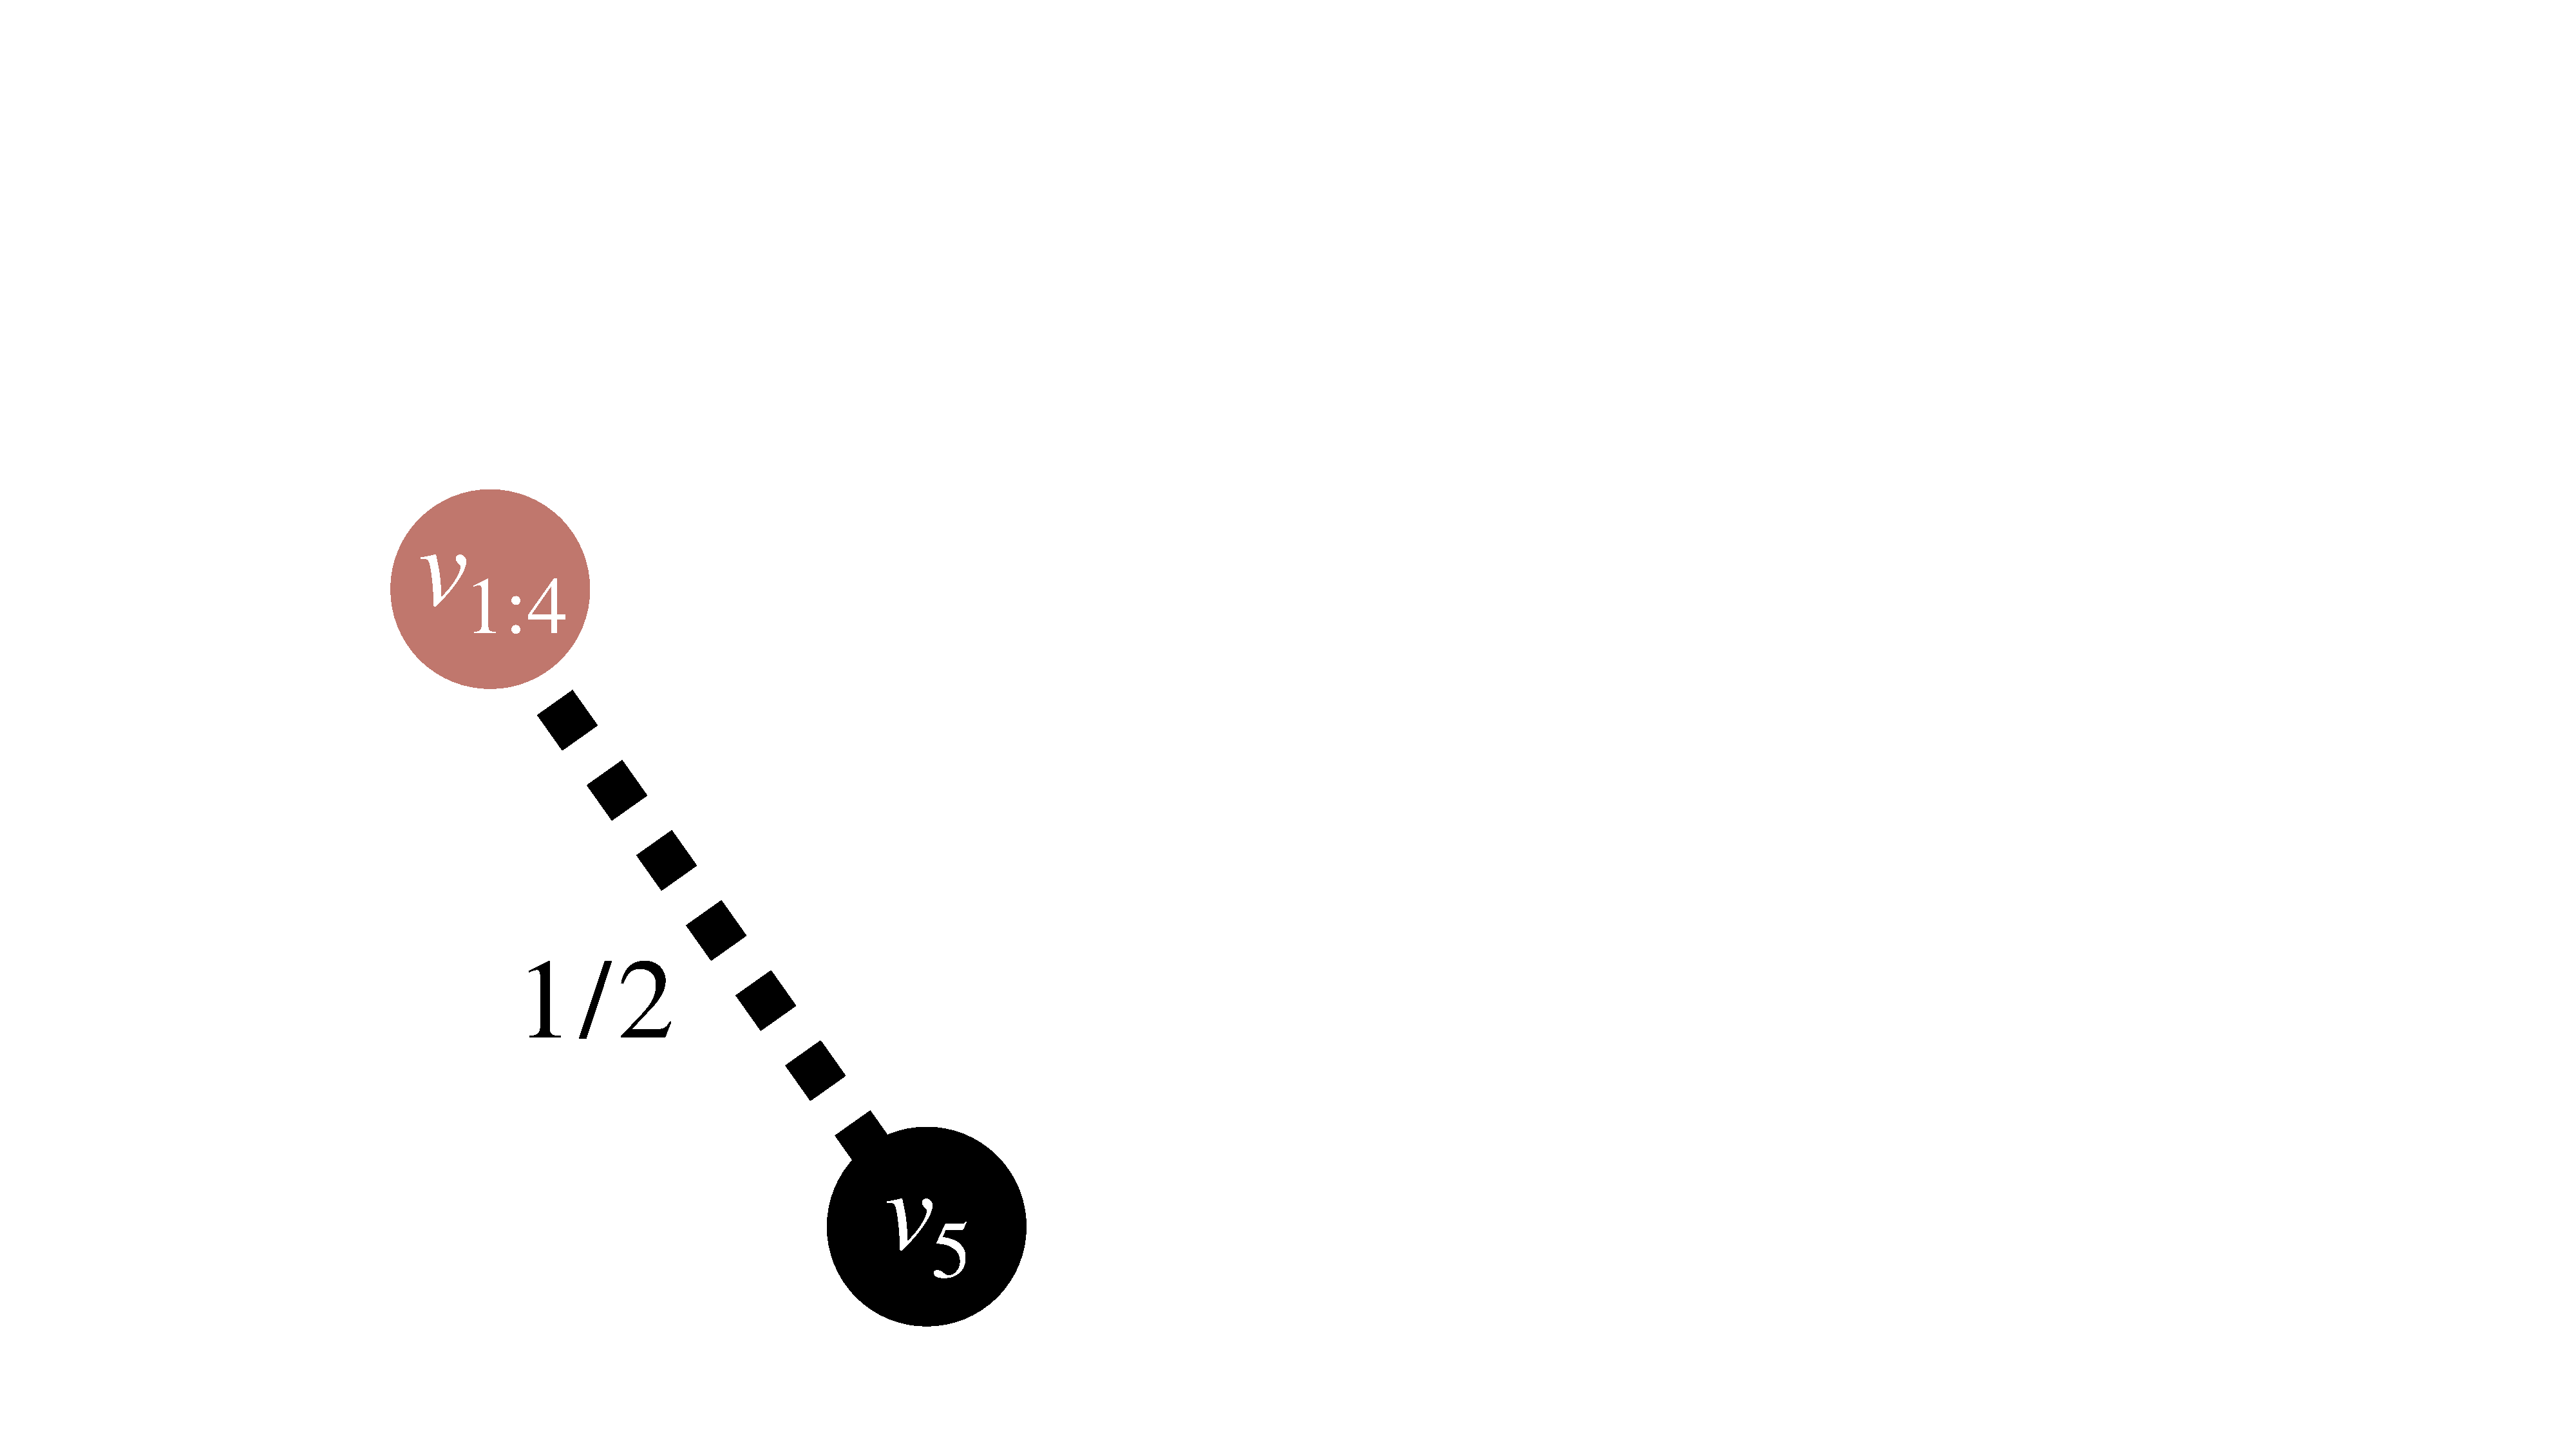
\includegraphics[width=\textwidth,trim=0mm 0mm 320mm 0mm, clip]{./figures/hacMerge4.pdf}
        \caption{3 merges.}\label{sfig:hacMerge4}
    \end{subfigure}   \hfill
        \begin{subfigure}[b]{0.19\textwidth}
        \centering
        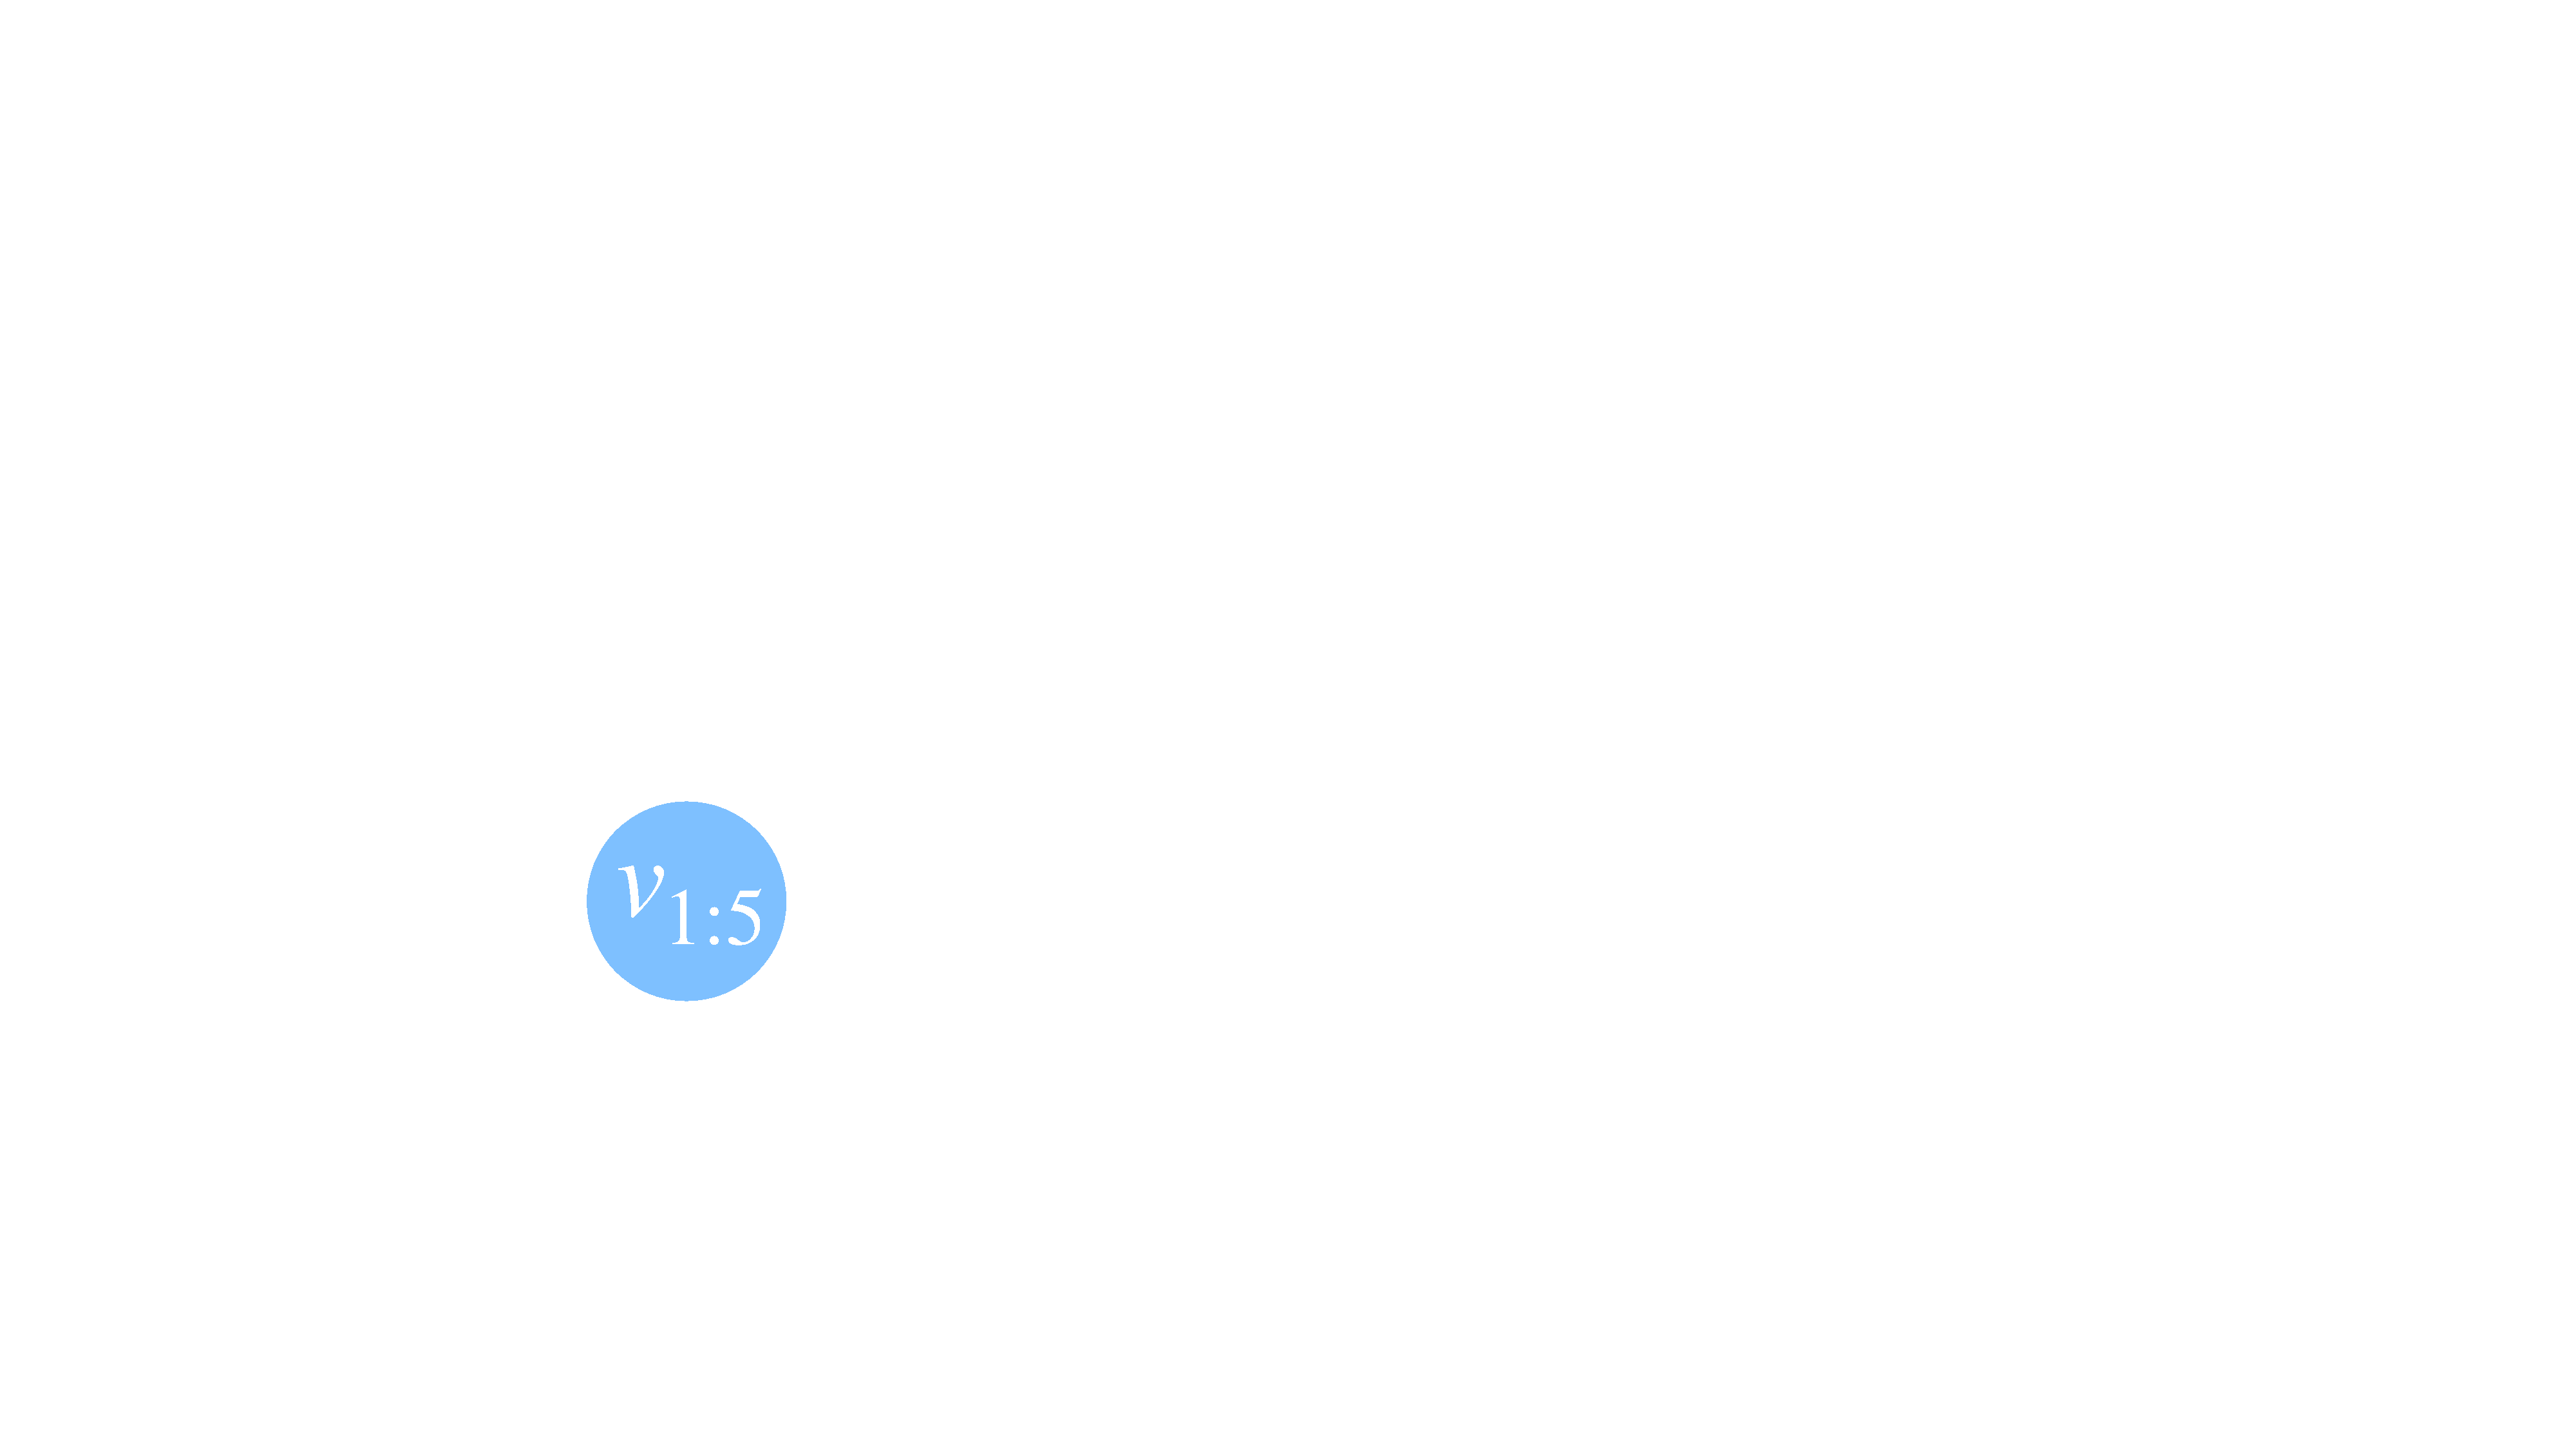
\includegraphics[width=\textwidth,trim=0mm 0mm 320mm 0mm, clip]{./figures/hacMerge5.pdf}
        \caption{4 merges.}\label{sfig:hacMerge5}
    \end{subfigure}   % \hfill
    \vspace{-0.5em}
    \caption{An example of average linkage HAC run on an input graph $G$ where we imagine we contract merged clusters. Intermediate vertices labeled with the vertices of $G$ their corresponding cluster contains. Edges labeled with their weight and next merged edge is dashed. } \label{fig:HACMerge}
\end{figure}

The output of HAC is a \emph{dendrogram}---a rooted binary tree representing the cluster merges performed by the algorithm.
Every node of the dendrogram is a cluster built by the algorithm.
There are exactly $|V|$ leaves corresponding to the single-element clusters that are formed in the beginning of the algorithm.
Whenever two clusters $C_1$ and $C_2$ are merged, we add to the dendrogram a new node $C_1 \cup C_2$ whose children are $C_1$ and $C_2$. See \Cref{sfig:hac3} for the dendrogram of \Cref{fig:HACMerge}.


\newcommand{\forkins}{\texttt{fork}}
\newcommand{\insend}{\texttt{end}}
\newcommand{\allocateins}{\texttt{allocate}}
\newcommand{\freeins}{\texttt{free}}
\newcommand{\mpram}{MT-RAM}
\newcommand{\thread}{thread}
\newcommand{\bfmodel}{binary-forking model}

%When analyzing parallel algorithms we 
We use the classic multithreaded model~\cite{BL98,ABP01,blelloch2020optimal} (formally, the MP-RAM~\cite{blelloch2020optimal}) to analyze the parallel algorithms.
%\hnote{Thread and fork macros not defined.}
We assume a set of \thread{}s that share the memory.
Each \thread{} acts like a sequential RAM plus a \forkins{} instruction  that forks two new child threads.
When a thread performs a fork, the two child threads can both start by running their next instructions, and the original thread is suspended until both children terminate.
A computation starts with a single root thread and finishes when that root thread finishes.
A parallel for-loop can be viewed as executing \forkins{}s for a logarithmic number of levels.
A computation can thus be viewed as a DAG (directed acyclic graph).
We say the {\em work} is the total number of operations in this DAG and {\em span (depth)} is equal to the longest path in the DAG.
We note that computations in this model can be cross-simulated in standard variants of the PRAM model in the same work (asymptotically), and losing at most a single logarithmic factor in the depth~\cite{blelloch2020optimal}.
% We use the $\mathsf{prefix\text{-}sum}$ primitive to 



\begin{algorithm}[t]
\caption{Average linkage HAC---static graph version.}\label{alg:staticgraph}
\KwIn{$G = (V, E, w)$}
\SetKwFunction{FSim}{Similarity}
\SetKwFunction{FHac}{HAC}
\SetKwProg{Fn}{Function}{:}{}

\Fn{\FSim{$C_1, C_2, w$}}{
\Return $\sum_{x \in C_1, y \in C_2} w(x,y) / (|C_1| \cdot |C_2|)$
}

\Fn{\FHac{$G$}}{
$\clustering \gets$ clustering where each vertex of $G$ is in a separate cluster\\
\While{$\exists_{C_1, C_2 \in \clustering}$ s.t. $C_1 \neq C_2$ and $\FSim(C_1, C_2, w) > 0$}{
$(C_1, C_2) = \argmax_{(C_1, C_2) \in \clustering \times \clustering} \FSim(C_1, C_2, w)$\\
$\clustering := (\clustering \setminus \{C_1, C_2\}) \cup \{C_1 \cup C_2\}$.
}
}
\end{algorithm}

\begin{algorithm}[t]
\caption{Average linkage HAC---graph contraction version.}\label{alg:contractions}
\KwIn{$G = (V, E, w)$}
\SetKwFunction{FSim}{Similarity}
\SetKwFunction{FHac}{HAC}
\SetKwProg{Fn}{Function}{:}{}

\Fn{\FSim{$x, y, w, S$}}{
\Return $w(x,y) / (S(x) \cdot S(y))$
}

\Fn{\FHac{$G$}}{
$S := $ a function mapping each element of $V$ to 1\\
\While{$\exists_{xy \in E}$ s.t. $\FSim(x, y, w, S) > 0$}{
$xy = \argmax_{xy \in E} \FSim(x, y, w, S)$\\
Contract $x$ with $y$ in G creating a vertex $z$. The parallel edges that are created are merged into a single edge whose weight is the sum of the merged edge weights. Any resulting self-loops are removed.\\
Set $S(z) := S(x) + S(y)$
}
}
\end{algorithm}

\section{An \texorpdfstring{\boldmath$\Omega(n^{3/2 - \epsilon})$}{Omega(n\^(3/2-epsilon))} Conditional Lower Bound for Average Linkage HAC}\label{sec:worklb}

In this section, we show an $\Omega(n^{3/2 - \epsilon})$ conditional lower bound on the time required to solve average linkage HAC on general weighted graphs. Specifically, we show this lower bound assuming the Combinatorial Boolean Matrix Multiplication (BMM) conjecture, a central conjecture in fine-grained complexity about the time required to multiply two $n \times n$ boolean matrices~\cite{williams2010subcubic, abboud2024faster}.
%\enote{We should define boolean matrix multiplication; we use it later in the corollary}

\begin{conjecture}[Combinatorial BMM]\label{conj:bmm}
Combinatorial algorithms cannot solve Boolean Matrix Multiplication in time $O(n^{3-\epsilon})$ for $\epsilon > 0$.
\end{conjecture}
\noindent We refer to~\cite{abboud2024faster} for an in-depth discussion of the somewhat informal notion of ``combinatorial'' algorithms and more on Conjecture~\ref{conj:bmm} and its history.

In this work we will make use of an equivalent characterization of the BMM conjecture due to \cite{williams2010subcubic}. Specifically, \cite{williams2010subcubic} shows that the BMM problem is sub-cubically equivalent to the Triangle Detection problem: the problem of deciding whether or not an input graph $G$ contains a triangle (i.e., cycle of $3$ vertices). The following summarizes this result.
\begin{theorem}[Theorem 1.3 of \cite{williams2010subcubic}]\label{thm:bmmeq}
    Combinatorial algorithms cannot solve Triangle Detection in time $O(n^{3-\epsilon})$ for  $\epsilon > 0$ unless \Cref{conj:bmm} is false.
\end{theorem}
Thus, we give a reduction from Triangle Detection to average linkage HAC. Our reduction will quadratically increase the number of vertices of the input Triangle Detection instance, and therefore give an $\Omega(n^{3/2 - \epsilon})$ lower bound for average linkage HAC. In the rest of this section, we show the following quadratic-blowup reduction from Triangle Detection to average linkage HAC.
%

\begin{theorem}\label{thm:lbreduction}
Given a Triangle Detection instance on graph $G$ with $t$ vertices and $m$ edges, there is a reduction that runs in $O(t^2)$ time and constructs an instance of average linkage HAC on graph $G'$ with $t + t^2$ vertices and $t^2 + m$ edges. 
Furthermore, given the sequence of merges performed by average linkage HAC on $G'$, we can solve Triangle Detection on $G$ in time $O(t^2)$.
\end{theorem}

As a corollary of this reduction and \Cref{thm:bmmeq}, we obtain the following conditional lower-bound on the running time of HAC.
%ruling out near-linear work algorithms for average linkage HAC on sparse graphs conditional on Conjecture~\ref{conj:bmm}.

\mainLowerSeq*

As a second corollary, we obtain a conditional lower-bound in terms of the optimal running time of matrix multiplication for two $n \times n$ binary matrices. 
Matrix multiplication can be solved in time $O(n^{\omega})$ where $2 \leq \omega < 2.3716$~\cite{williams2024new}. 
An extensive line of research on matrix multiplication over the past thirty years has only improved $\omega$ from $2.376$ to $2.3716$, with the current state-of-the-art being due to a very recent result of Williams et al.~\cite{williams2024new} (for a subset of the historical advances in this area see, e.g., \cite{coppersmith1982asymptotic, le2012faster, alman2021refined, williams2012multiplying}).
The fastest known algorithm for triangle detection works by simply reducing the problem to matrix multiplication and therefore runs in $O(n^{\omega})$ time.
Surprisingly, despite triangle detection only returning a single bit (whether a triangle exists or not in $G$), the problem can be used to give a sub-cubic reduction for boolean matrix multiplication (where the output is $n^2$ bits).
In particular, an algorithm for triangle detection running in time $O(n^{3-\delta})$ for some $\delta > 0$ yields an algorithm for matrix multiplication in time $O(n^{3-\delta/3})$~\cite{williams2010subcubic}.
Using this fact, we can derive a conditional lower bound based on the value of $\omega$.

\workmatmul*



%\lnote{Not very happy with the below formulation.}
%\hnote{How about we state a theorem about the  actual reduction and the quadratic blow-up, and then two corollaries about its implications? Also, in the corollary below, I would mention matrix multiplication rather than triangle detection. I would then add a couple of sentences for the non-familiar reader that, while we do not know if $\omega$ has to be greater than two, thirty years of extensive research has only improved it from 2.376 to 2.372.}
%Another consequence of our reduction is that a non-combinatorial algorithm for average linkage HAC running in $O(n^{\omega/2 - \epsilon})$ time for any $\epsilon > 0$ would imply an algorithm for triangle detection in $O(n^{\omega - \epsilon'})$ time for some $\epsilon' > 0$.

An interesting open question is whether there are faster non-combinatorial algorithms that can leverage fast matrix multiplication or Strassen-like techniques and improve over the $\Omega(n^{3/2 - \epsilon})$ barrier for combinatorial algorithms for average linkage HAC.

\subsection{Reduction}
We now prove Theorem~\ref{thm:lbreduction} by
giving a quadratic-time reduction from triangle detection to average linkage HAC.
The reduction is loosely inspired by a recent lower-bound result for multidimensional range queries~\cite{lau2021algorithms}.
%\knote{Mention that the LB is loosely based on the range-minimum paper}
The input to the reduction is an unweighted graph $G$ on $t$ vertices with $m$ edges; the problem is to detect whether $G$ has a triangle.
To do this, we will construct a HAC instance on an edge-weighted graph $G'$ with $t + t^2$ vertices and $t^2 + m$ edges. 
%\hnote{There are $t^2+t$ vertices, right?}
We will show that the specific way in which an exact HAC algorithm merges the edges in this instance reveals whether or not $G$ has a triangle.

\paragraph{Constructing $G'$}
Let $N_{G}(v)$ denote the neighbors of a vertex $v \in G$ (note that $v \notin N_{G}(v)$).
%\knote{incl/excl $v$?}
We define $G'$ as follows. 
We start by adding all vertices and edges from $G$, that is the $t$ vertices $v_1, \ldots, v_t$ from $G$, including all of their incident edges $N_{G}(v_i)$.
We call these the {\em core} vertices. 
The initail weight of the edges between any two core vertices is set to $1$.

In addition to the core vertices, we add an additional $t^2$ {\em leaf} vertices that we connect to the core vertices with specific edge weights.
We add the $t^2$ leaf vertices over a sequence of $t$ {\em rounds} where the $i$-th round connects one new leaf vertex to every core vertex.
The weights to the newly added leaves depend on the neighbors of the node $v_i$ in the original graph $G$, and are set as follows:
\begin{enumerate}[label=(\textbf{\arabic*})]
\item A core vertex $v_j$ is connected to its new leaf with an edge of weight $(1/i) - \epsilon$ if $v_j \in N_{G}(v_i)$.\label{typeone}
\item A core vertex $v_j$ is connected to its new leaf with an edge of weight $(1/i) + \epsilon$ if $v_j \notin N_{G}(v_i)$.\label{typetwo}
\end{enumerate}

\noindent See \Cref{fig:HACSeqRed} for an illustration of our reduction.
\begin{figure}[h]
    \centering
    \begin{subfigure}[b]{0.25\textwidth}
        \centering
        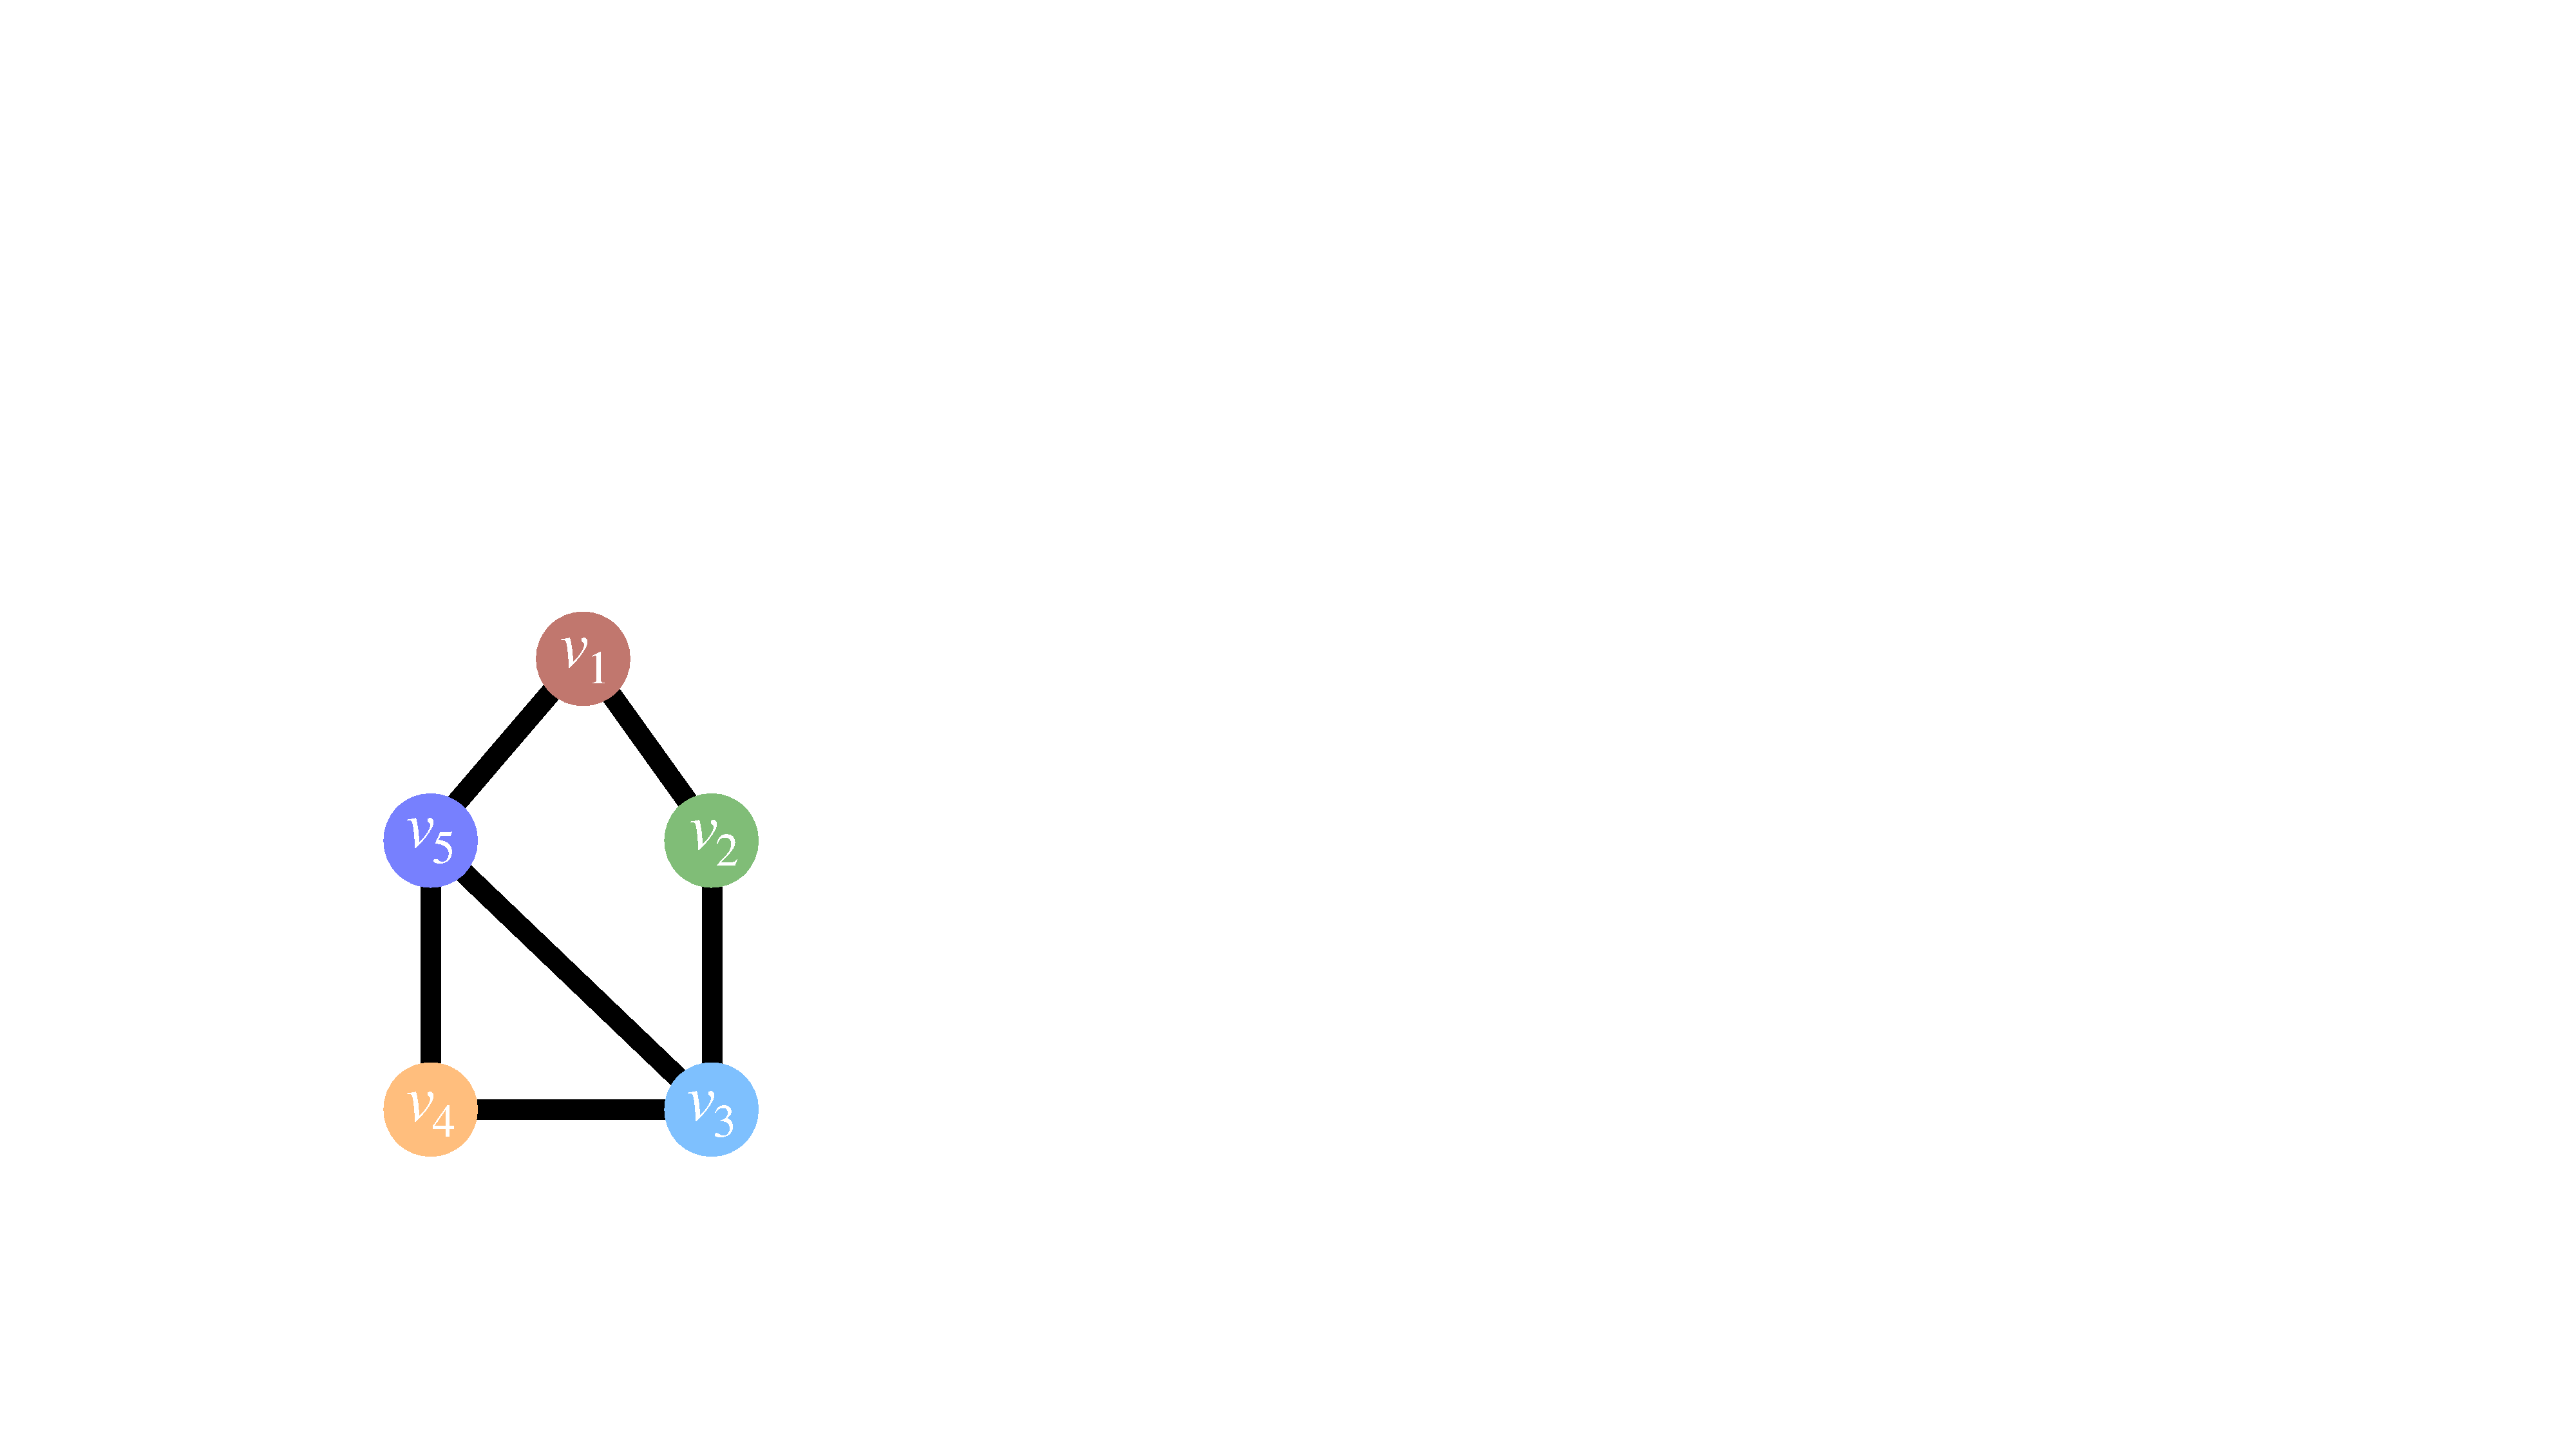
\includegraphics[width=\textwidth,trim=0mm 0mm 370mm 160mm, clip]{./figures/CBMMRed1.pdf}
        \caption{Input $G$.}\label{sfig:CBMMRed1}
    \end{subfigure} \hfill
       \begin{subfigure}[b]{0.25\textwidth}
        \centering
        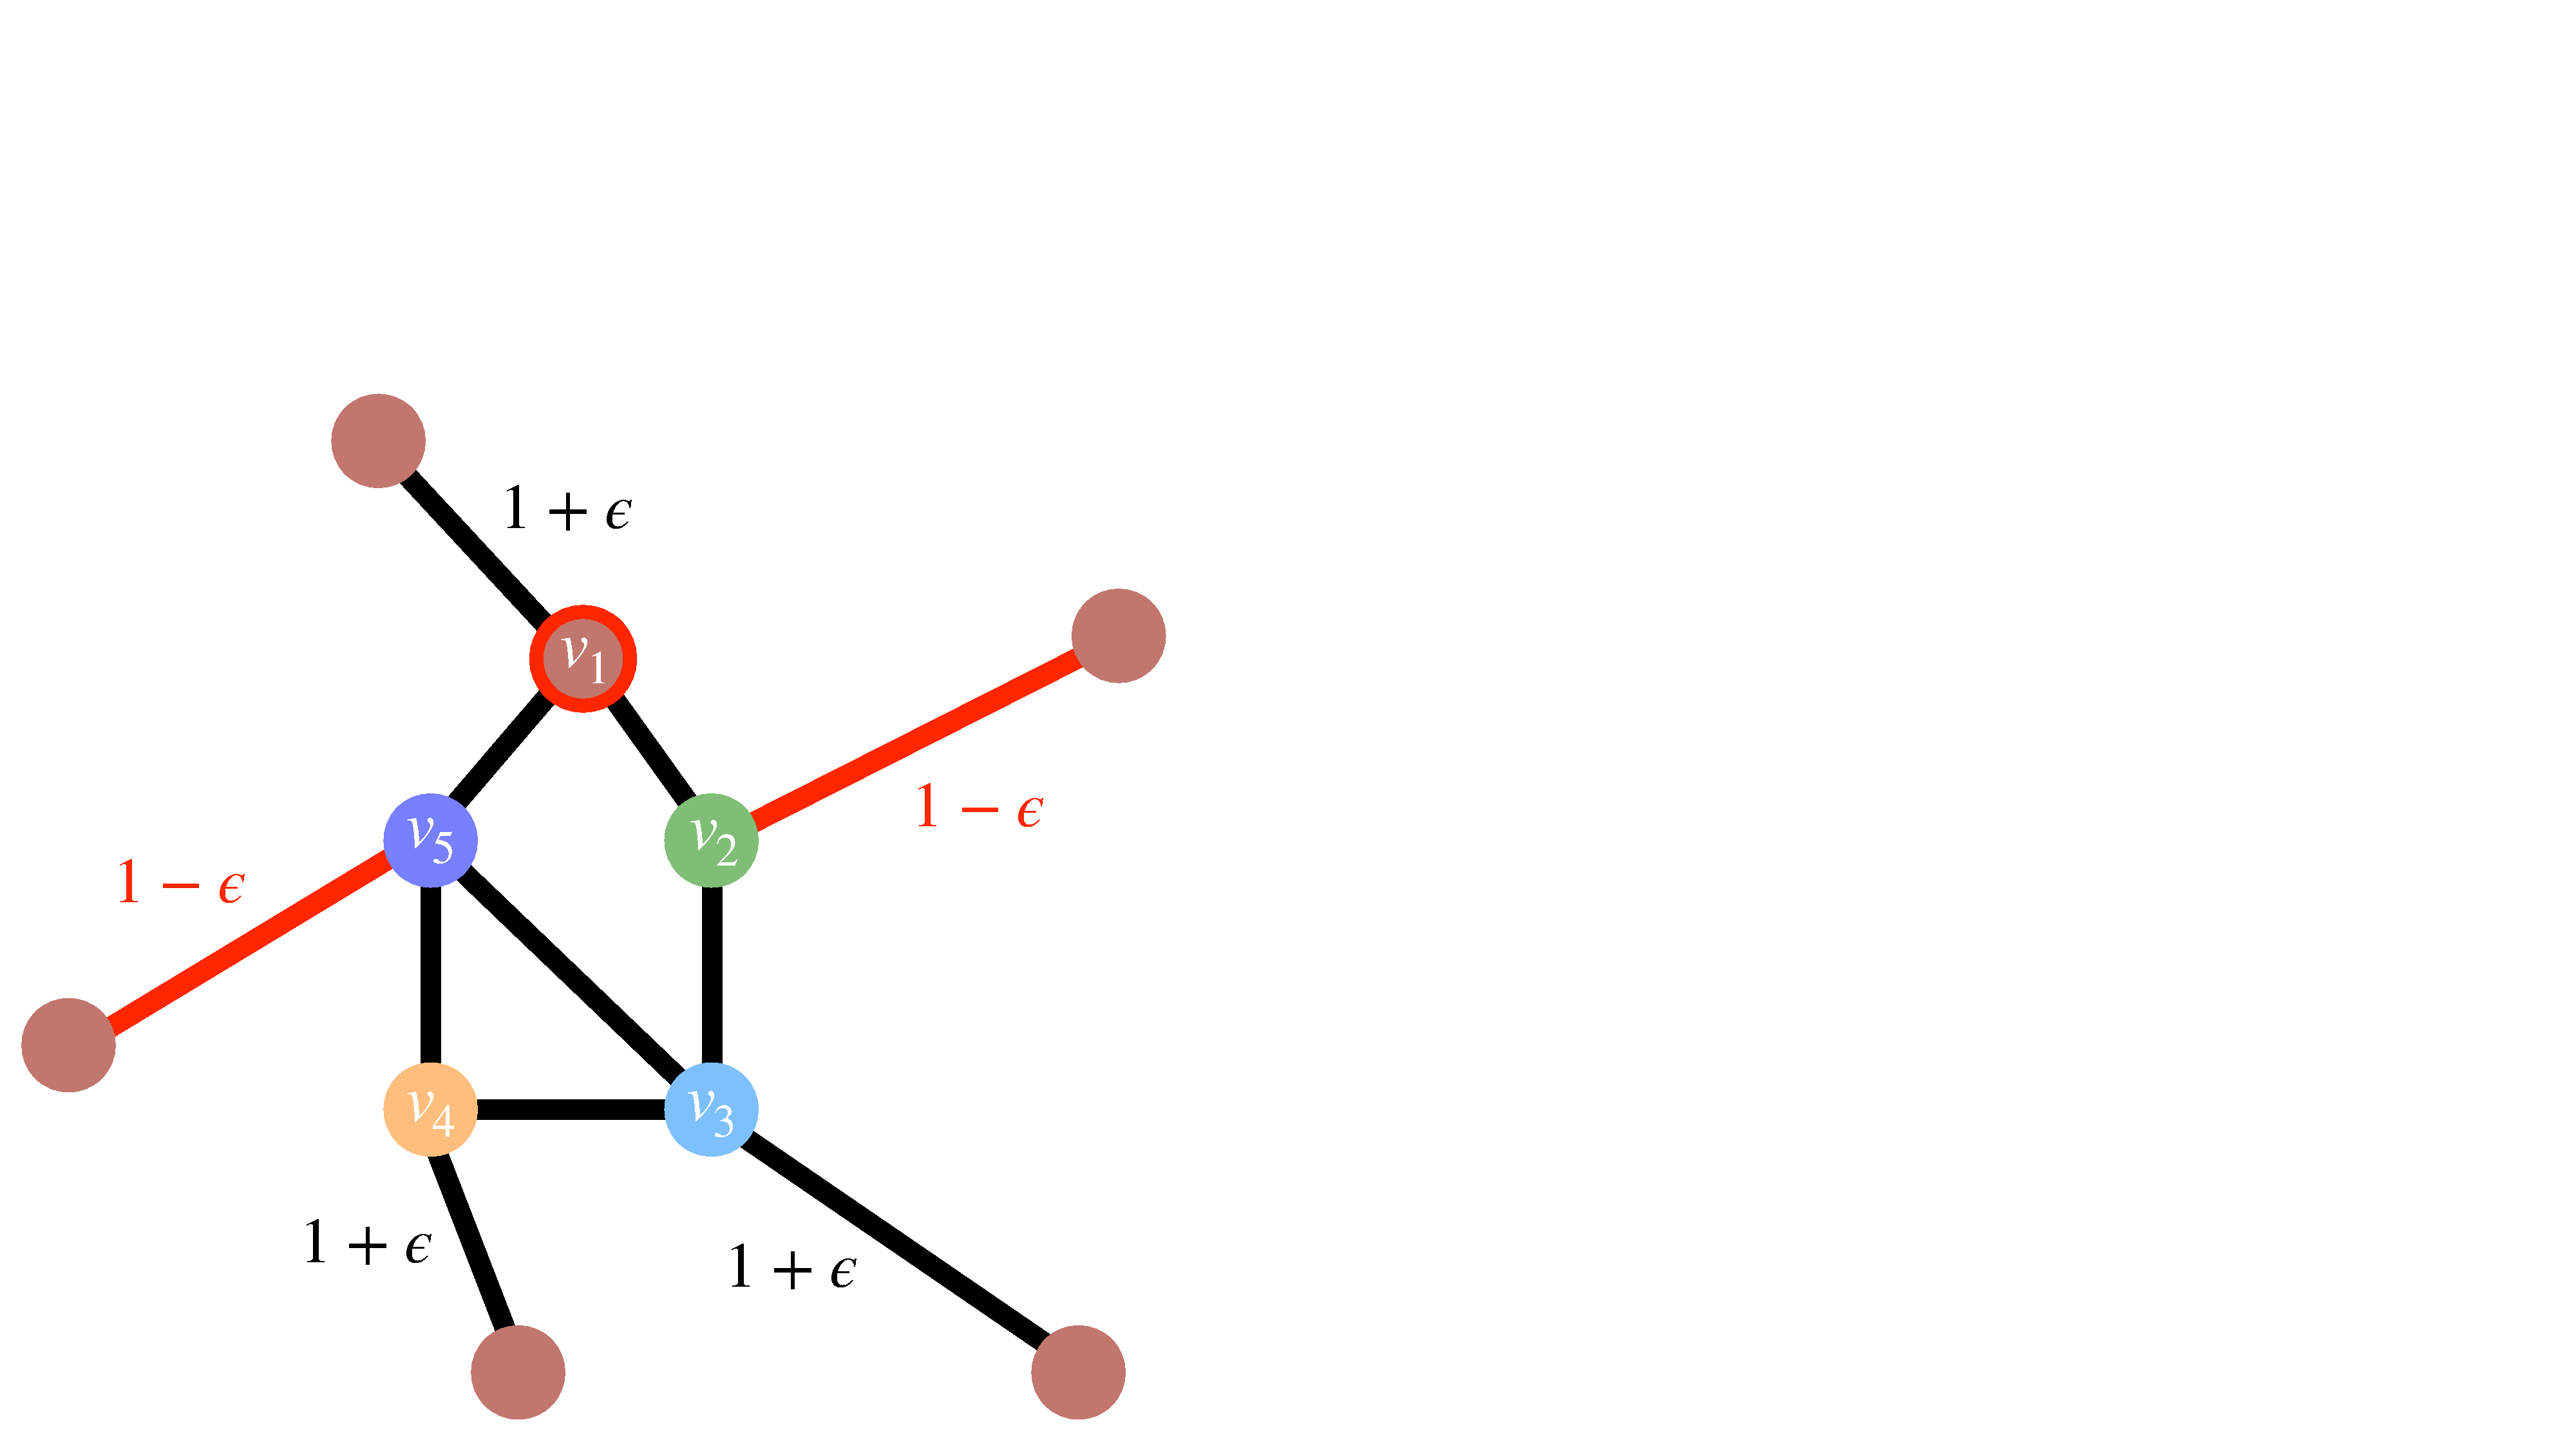
\includegraphics[width=\textwidth,trim=0mm 0mm 370mm 80mm, clip]{./figures/CBMMRed2.pdf}
        \caption{Round $1$.}\label{sfig:CBMMRed2}
    \end{subfigure} \hfill
       \begin{subfigure}[b]{0.25\textwidth}
        \centering
        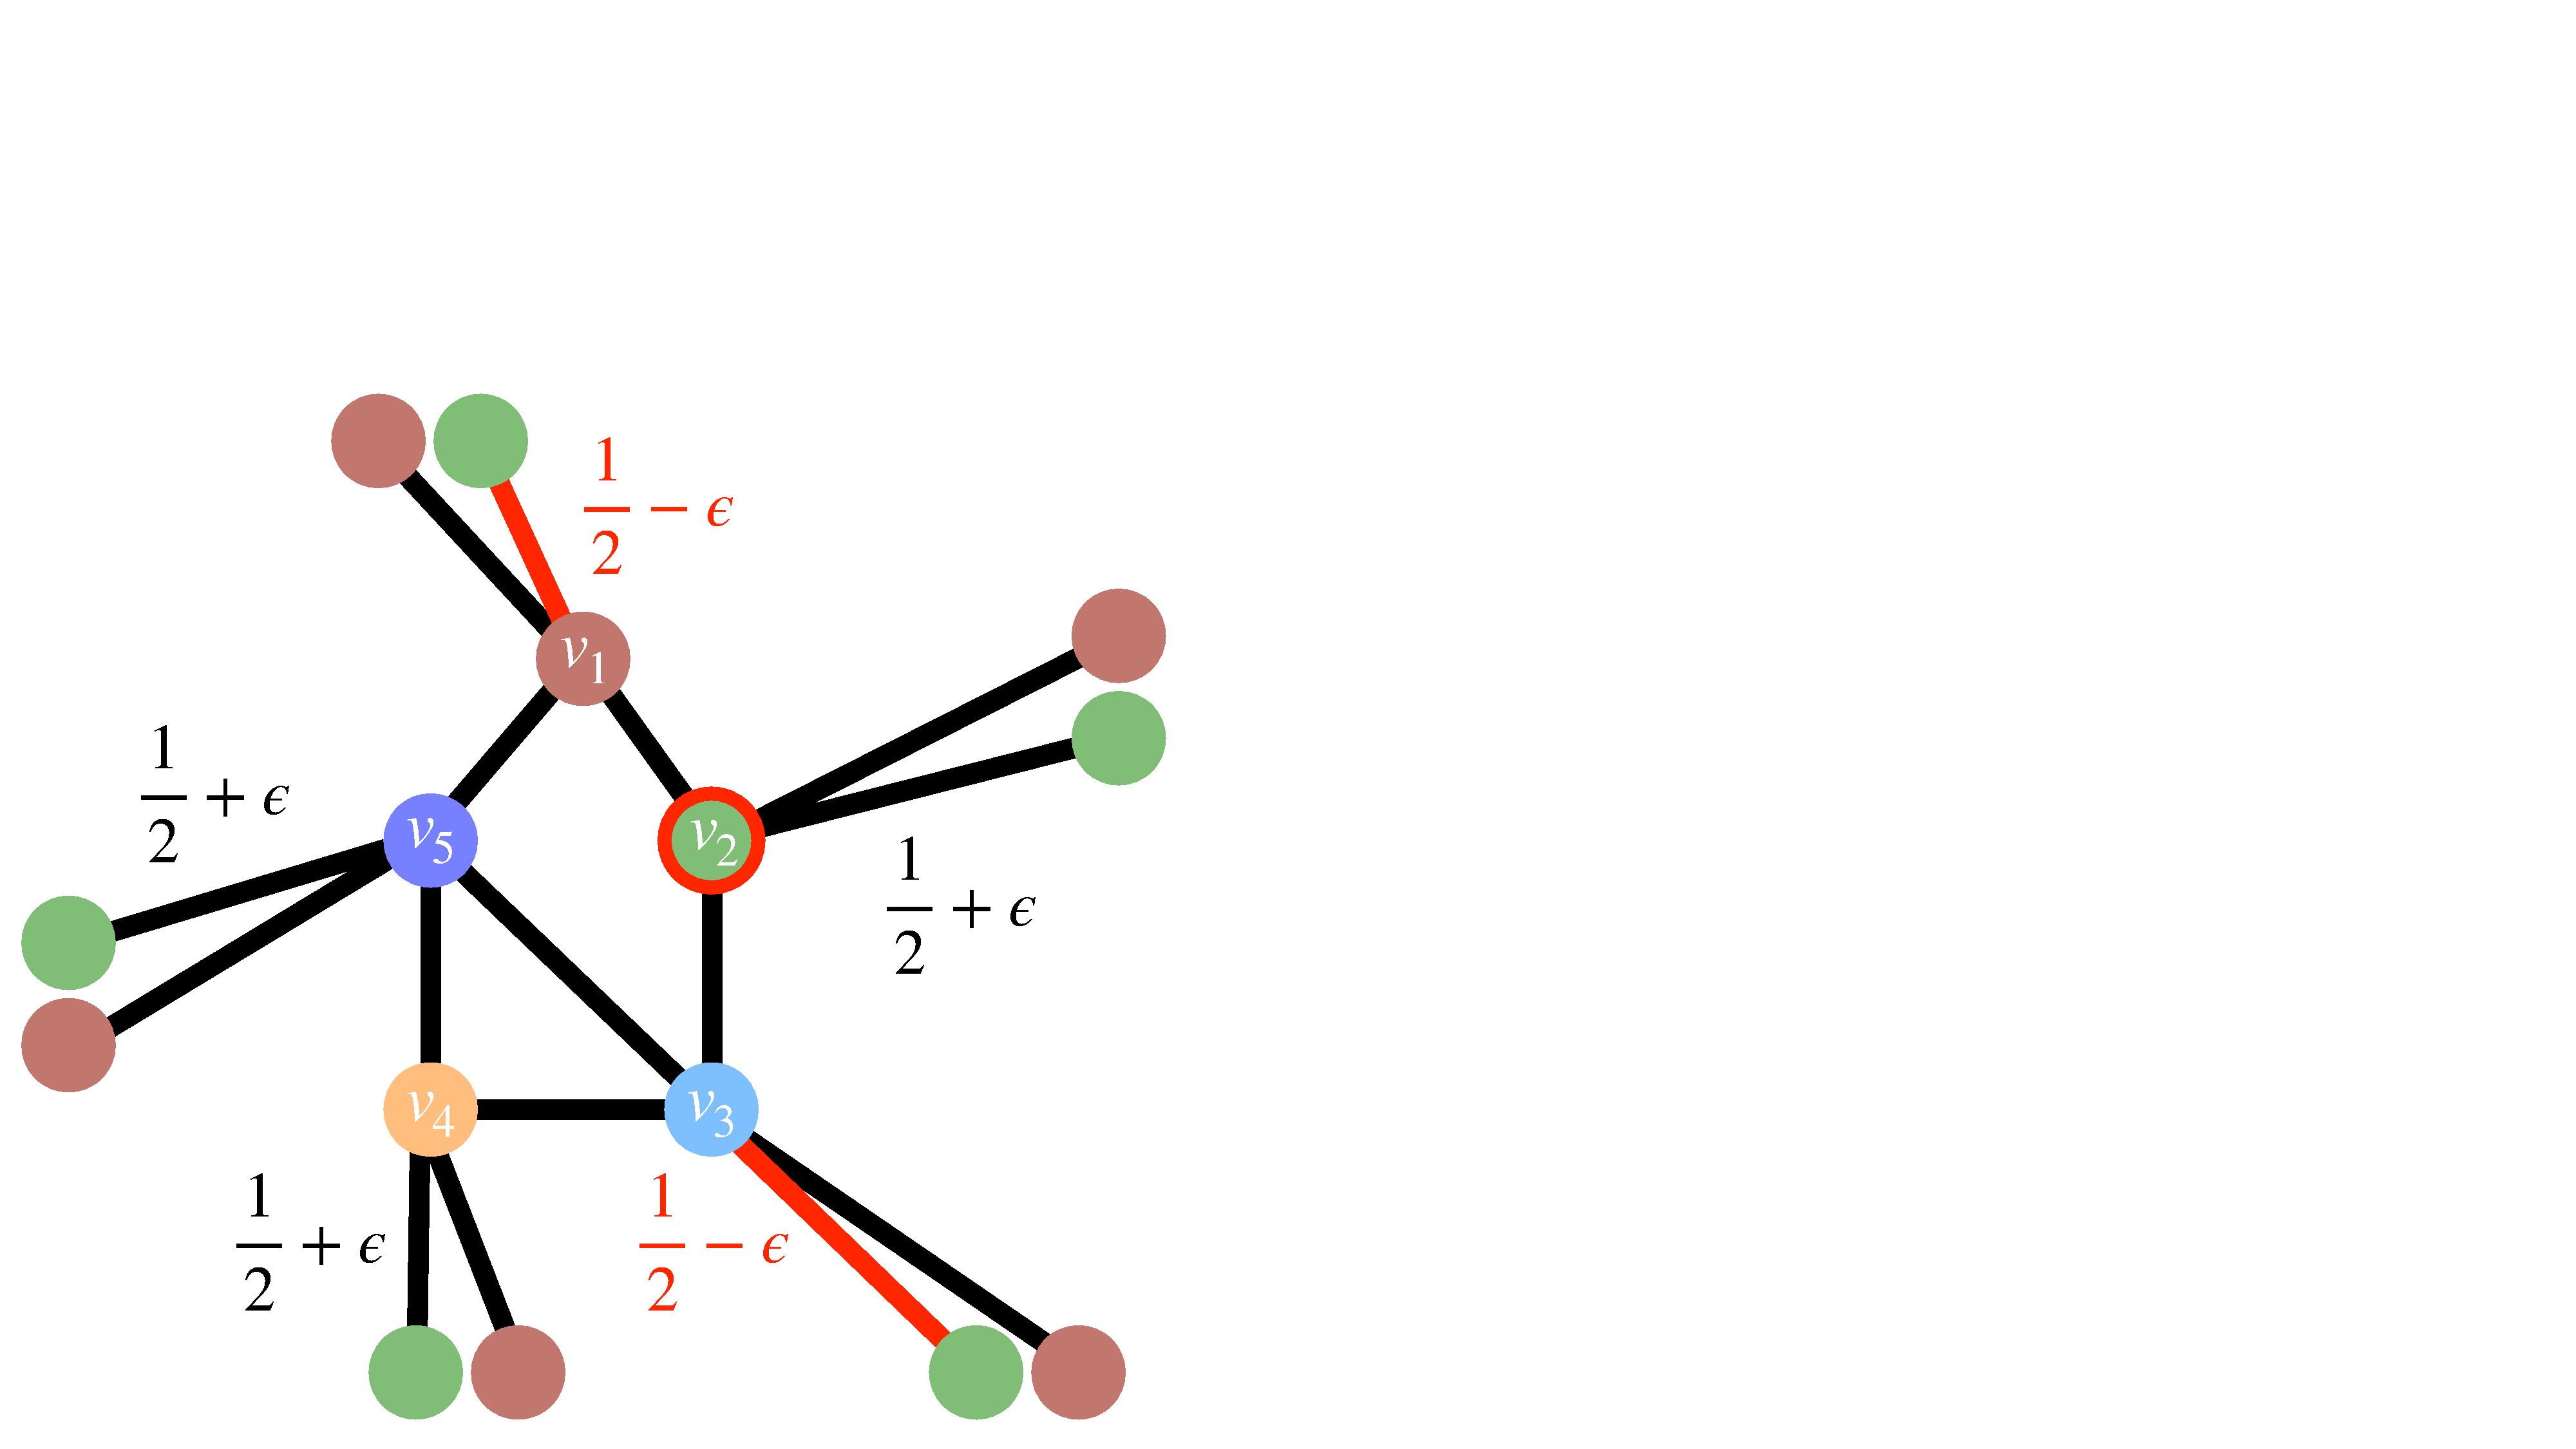
\includegraphics[width=\textwidth,trim=0mm 0mm 370mm 80mm, clip]{./figures/CBMMRed3.pdf}
        \caption{Round $2$.}\label{sfig:CBMMRed3}
    \end{subfigure} \hfill
    \begin{subfigure}[b]{0.25\textwidth}
        \centering
        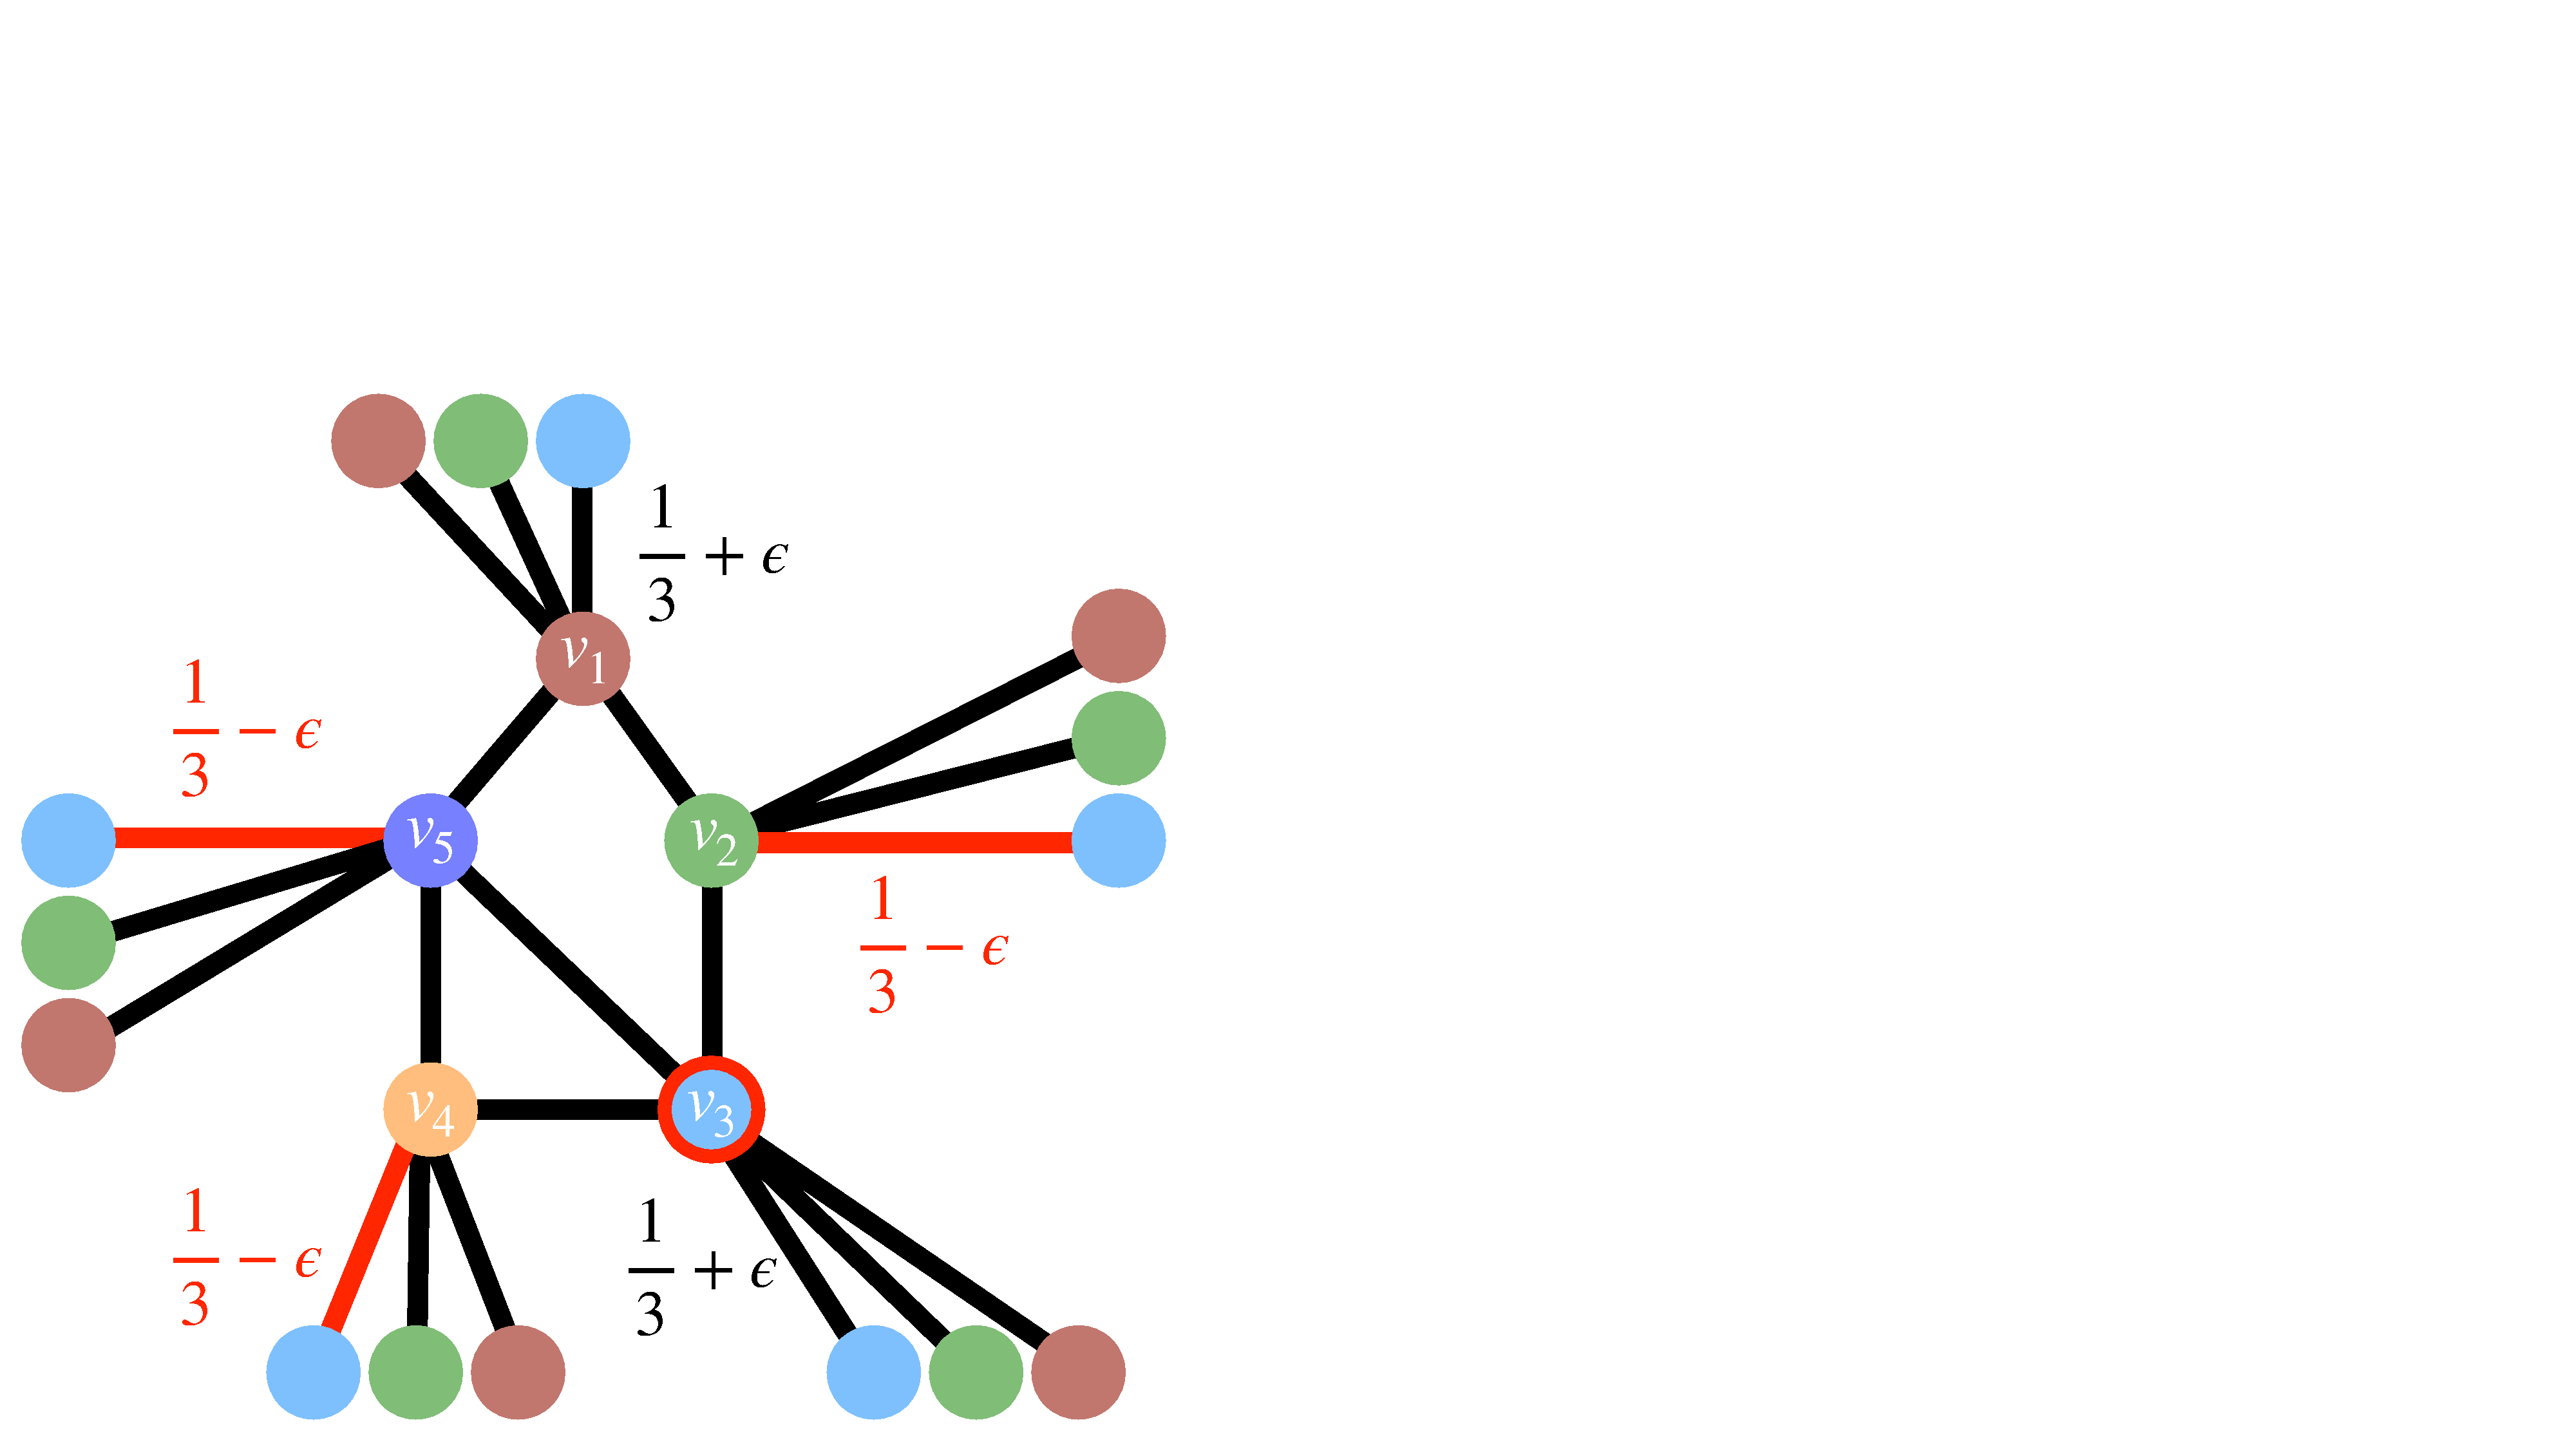
\includegraphics[width=\textwidth,trim=0mm 0mm 370mm 80mm, clip]{./figures/CBMMRed4.pdf}
        \caption{Round $3$.}\label{sfig:CBMMRed4}
    \end{subfigure} \hfill
    \begin{subfigure}[b]{0.25\textwidth}
        \centering
        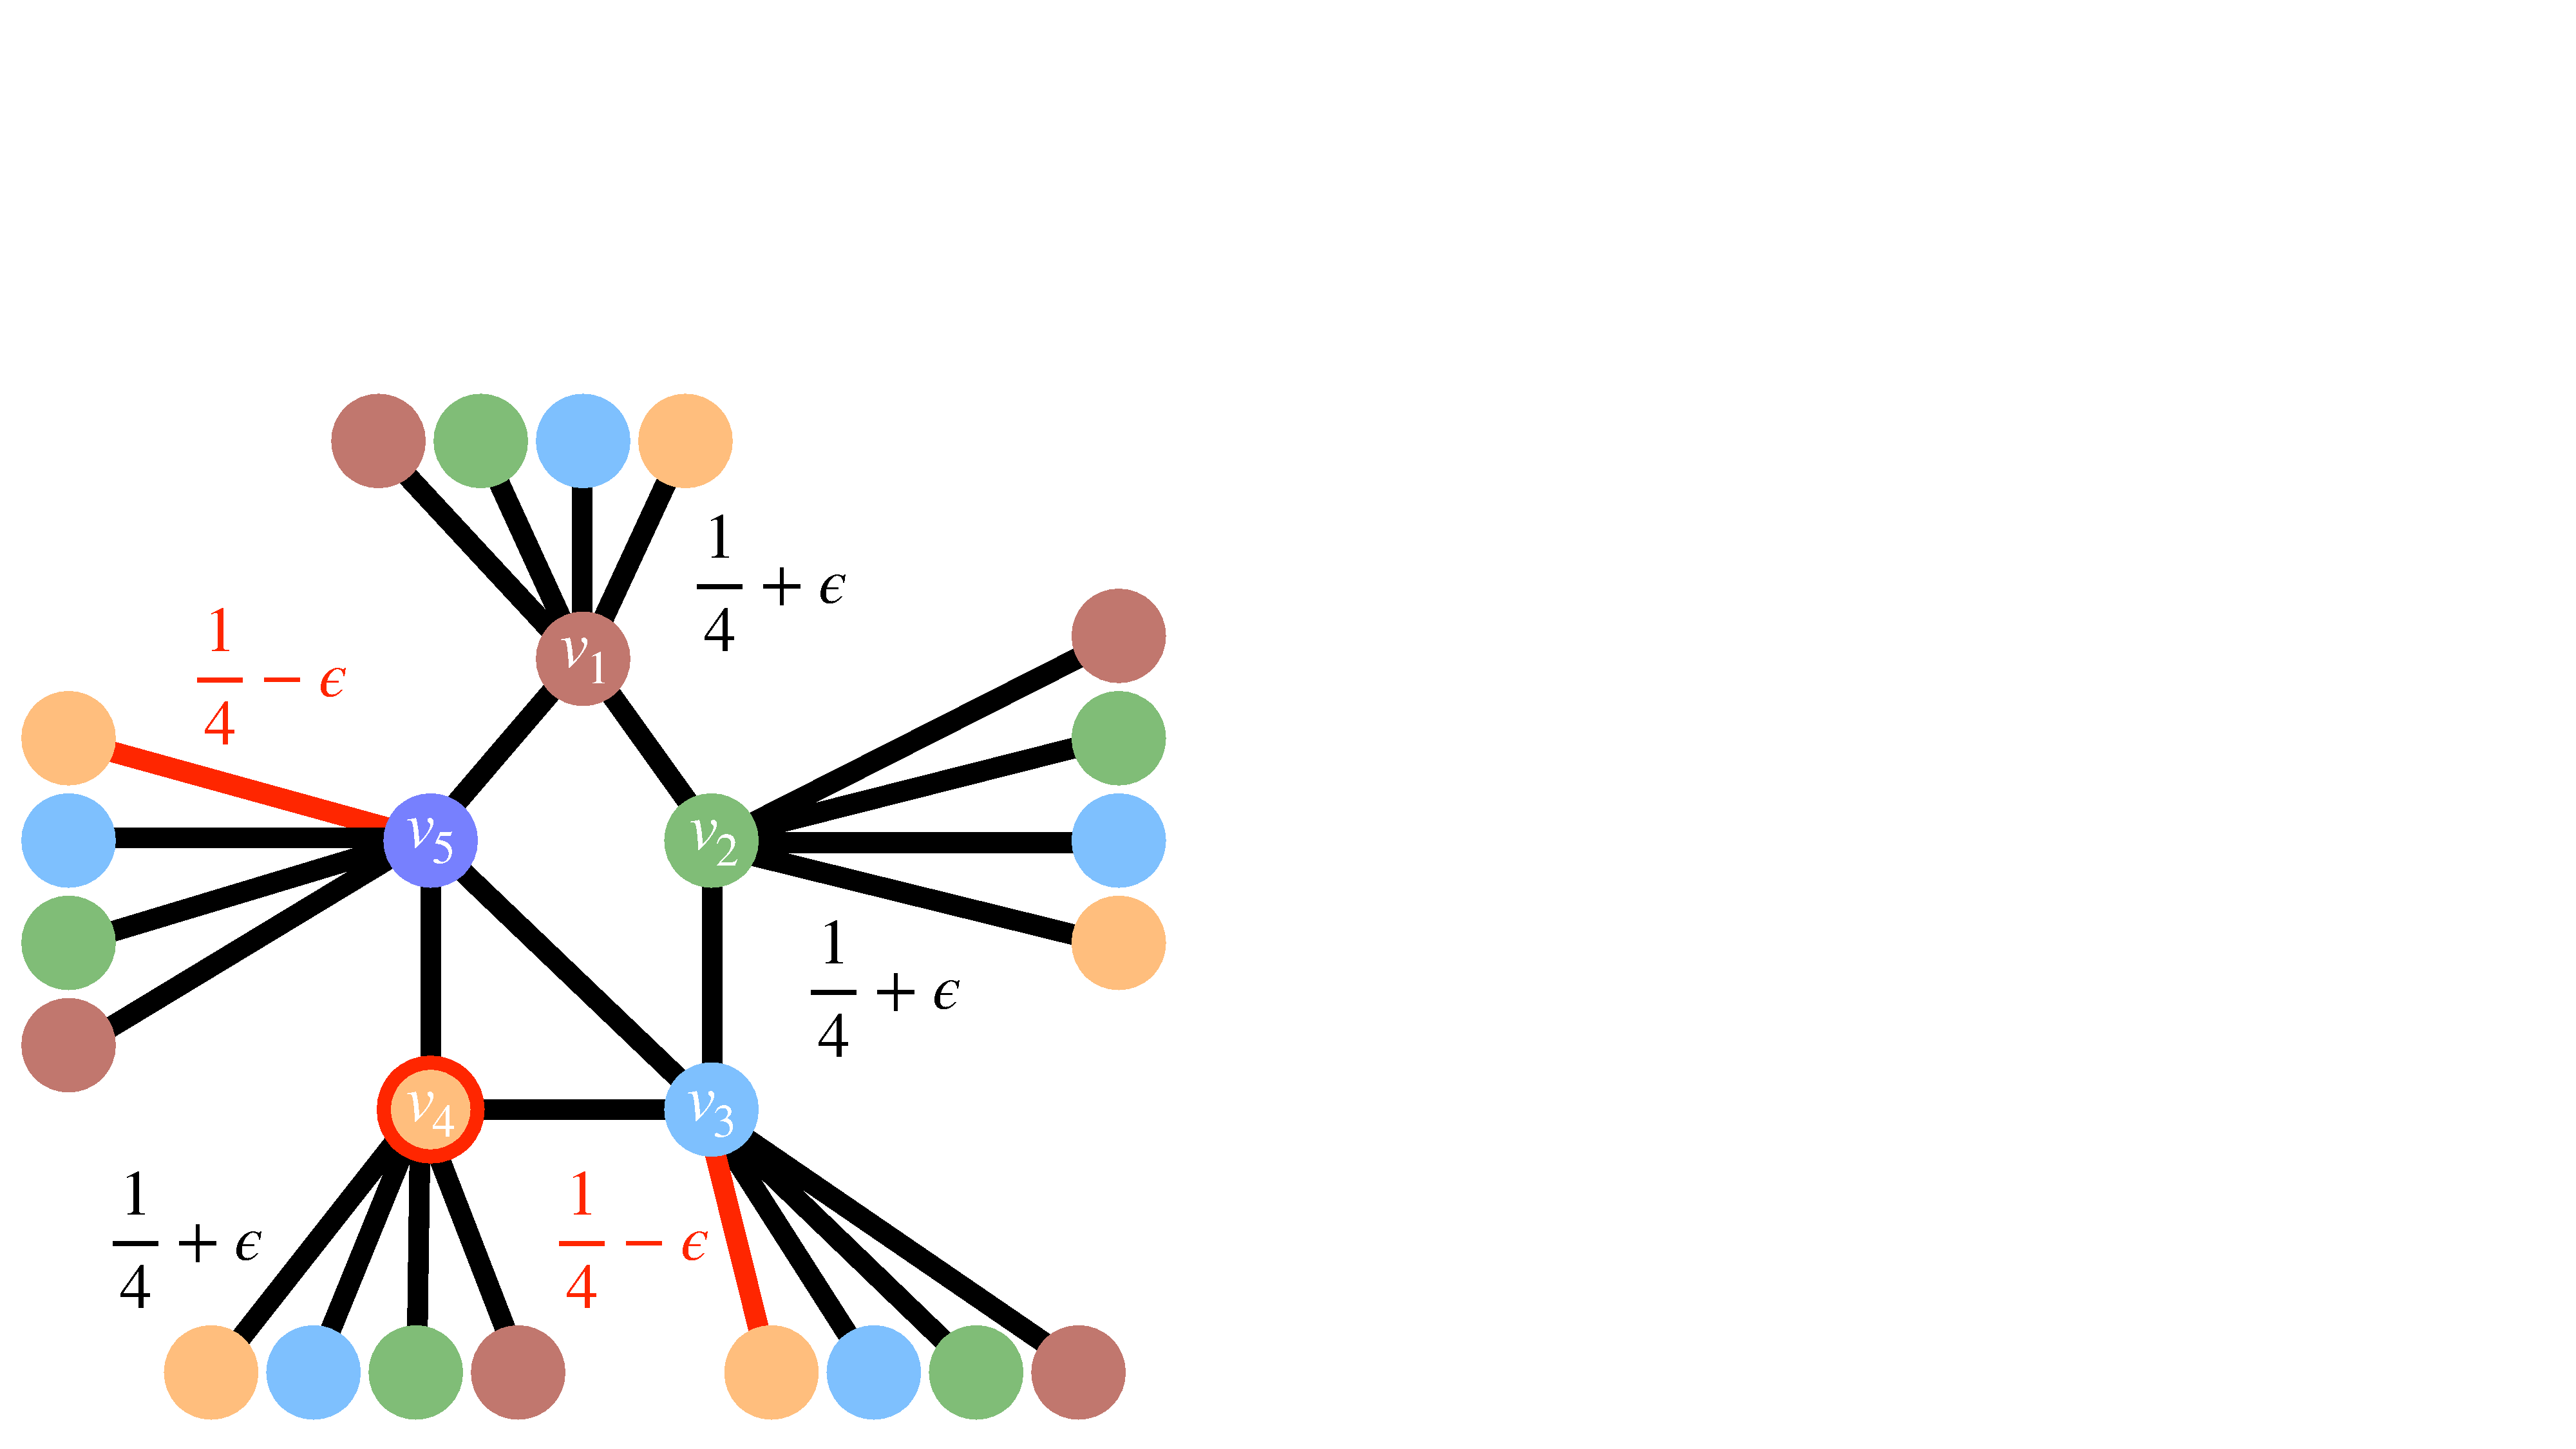
\includegraphics[width=\textwidth,trim=0mm 0mm 370mm 80mm, clip]{./figures/CBMMRed5.pdf}
        \caption{Round $4$.}\label{sfig:CBMMRed5}
    \end{subfigure} \hfill
    \begin{subfigure}[b]{0.25\textwidth}
        \centering
        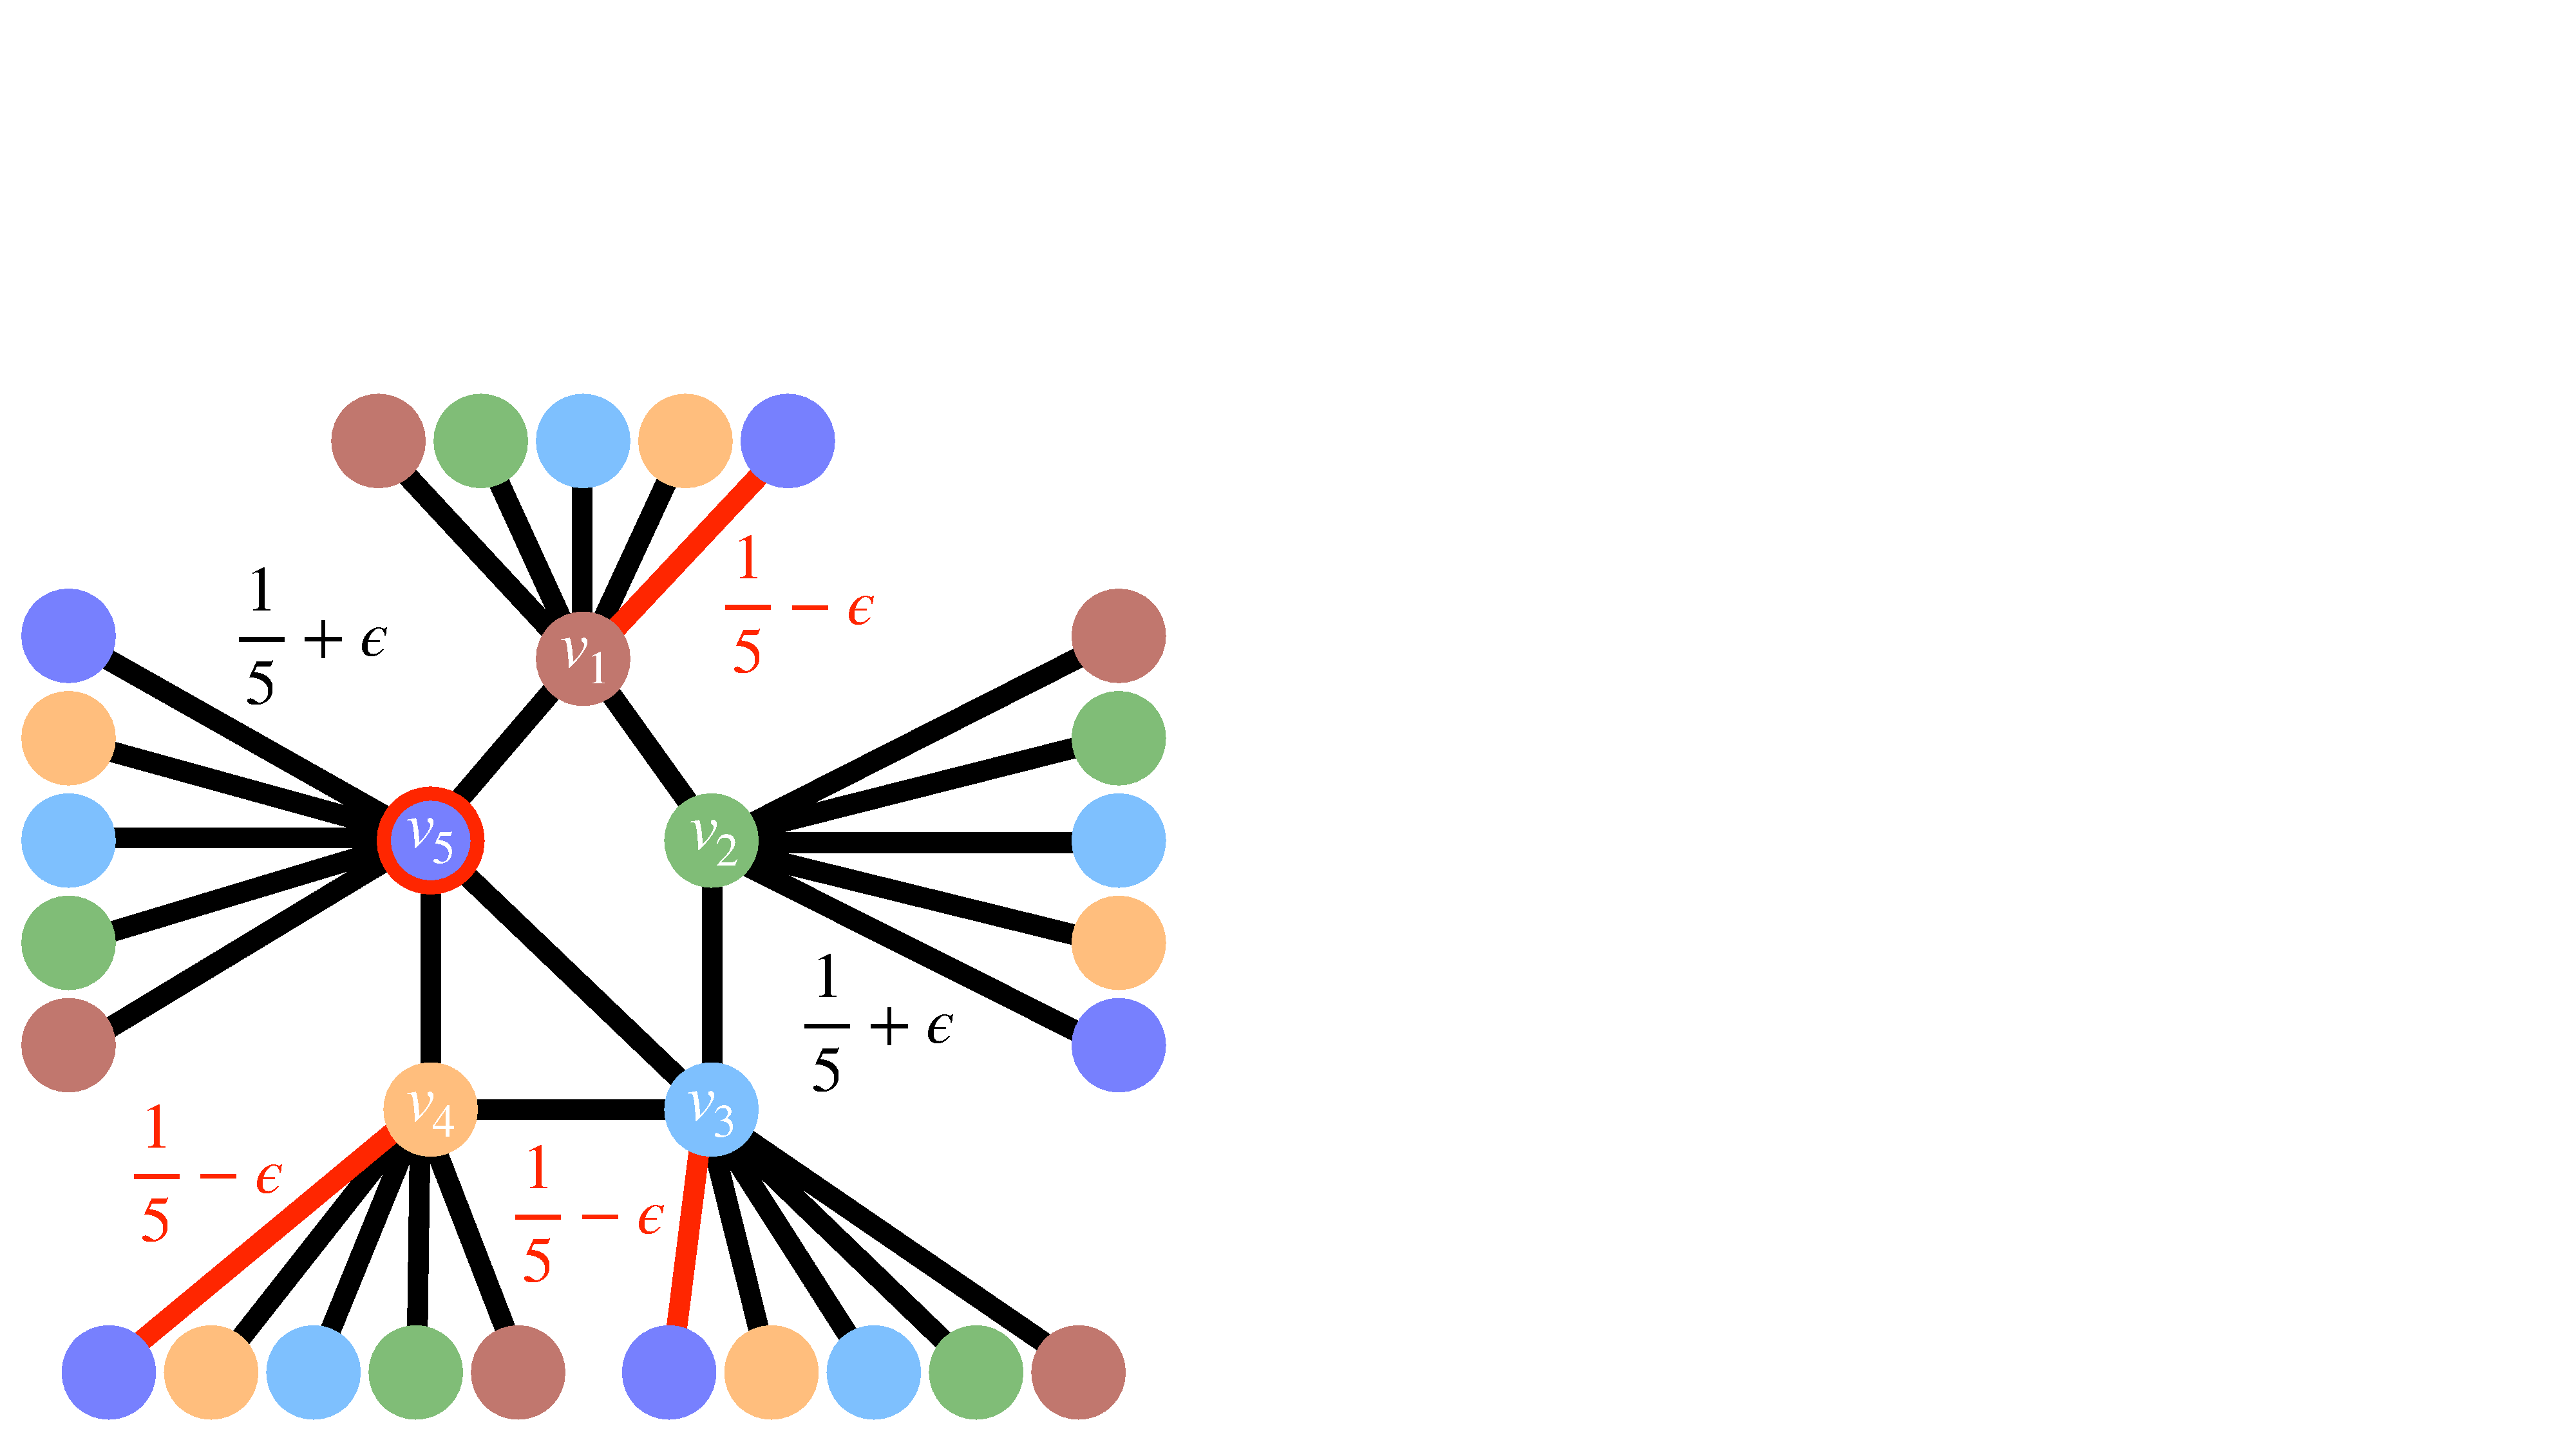
\includegraphics[width=\textwidth,trim=0mm 0mm 370mm 80mm, clip]{./figures/CBMMRed6.pdf}
        \caption{Round $5$.}\label{sfig:CBMMRed6}
    \end{subfigure} \hfill
    \caption{Our triangle detection reduction where we compute $G'$ from $G$ by adding $t=5$ nodes over $t$ rounds. \ref{sfig:CBMMRed6} gives $G'$. Each node labeled according to its round and corresponding vertex in $G$. Edges labelled with their weight in the round they are added (edges of $G$ have weight $1$). For the $i$th round we highlight in red $v_i$ and the edges added with weight $1/i-\epsilon$.} \label{fig:HACSeqRed}
\end{figure}


\paragraph{Running HAC on $G'$}
Having defined $G'$, let us consider the merges that the exact HAC algorithm will make on this instance.
In this section, for succinctness we use {\em weight} to refer to the normalized (i.e., average linkage) weight.
HAC will begin by merging the maximum weight edges.
The maximum weight initially depends on the structure of $N_{G}(v_1)$.
First, all core vertices that are not in $N_{G}(v_1)$ will merge with their round 1 leaves (since these edges have weight $1+\epsilon$) increasing their cluster size to $2$.
This leaves all core vertices in $N_{G}(v_1)$. Any edge in $G'$ between two such core vertices will have weight $1$, and will be merged next.
Crucially, any merge in this round with a weight of $1$ indicates a triangle incident on $v_1$ since the two core vertex endpoints of the edge must be contained in $N_{G}(v_1)$, hence connected by 
edges to $v_1$.
If no edges of weight $1$ merge, the remaining leaves that we added to core vertices in $N_{G}(v_1)$ merge into their neighboring core vertex.

Assuming we did not merge any weight $1$ edges in the first round, at this point the cluster size of each core vertex is $2$, and so the weight of any edge originally in $G$ (between two core vertices) will be $1/4$.
The edge weights to leaves in round $2$ will be $((1/2) \pm \epsilon)/2 = 1/4 \pm (\epsilon / 2)$, which is larger than $1/4$ for edges of Type~\ref{typetwo}.
Therefore, the same argument for how edges merge in round $1$ can be inductively applied to the next round.
The edge weights in round $i$ for edges between core vertices will be $1/i^2$, and by the same argument as before, the Type~\ref{typetwo} (Type~\ref{typeone}) edges will be larger (smaller) by $\epsilon/i$.
%\knote{maybe clarify that the edge weights in round $i$ are $1/i^2$}
As a result of how an exact average linkage HAC will merge the edges of $G'$, we obtain the following lemma:

\begin{lemma}
Consider the sequence of merges performed by the HAC algorithm on $G'$. If the merge sequence consists of $t^2$ merges, which first merge all leaf vertices, and only then makes merges between core vertices, then $G$ does not contain any triangles.
If the merge sequence merges any edge between two core vertices in the first $t^2$ merges, then $G$ contains a triangle.
\end{lemma}

\paragraph{Completing the Reduction}
We will now complete the proof of Theorem~\ref{thm:lbreduction}.
Suppose we are given an instance of \textsc{Triangle Detection} on $n$ vertices.
Conjecture~\ref{conj:bmm} implies that this instance cannot be solved by combinatorial algorithms in $O(n^{3-\epsilon})$ time for any $\epsilon > 0$.

Let the time complexity of HAC on a graph $G$ with $n$ vertices and $m$ edges be $T_{\mathsf{HAC}}(n,m)$.
Suppose HAC can be solved combinatorially in $O(n^{3/2 - \epsilon})$ time.
Given a \textsc{Triangle Detection} instance on $n$ vertices we create a graph $G'$ with $O(n^2)$ vertices and $O(n^2)$ edges, and run HAC on $G'$.
The running time of the reduction is $O(n^2)$, and the running time of HAC on $G'$ is $O((n^{2\cdot (3/2-\epsilon)}) = O(n^{3 - 2\epsilon})$, which will falsify Conjecture~\ref{conj:bmm} by \Cref{thm:bmmeq}.
Thus, conditional on Conjecture~\ref{conj:bmm}, there is no algorithm for HAC running in time $T_{\mathsf{HAC}}(n, m) = O(n^{3/2 - \epsilon})$ for any constant $\epsilon > 0$, completing the proof of Theorems~\ref{thm:lbreduction} and \ref{thm:worklb}. 
The same argument, under the assumption that triangle detection cannot be solved in $O(n^{\omega - \epsilon})$ time for any constant $\epsilon > 0$ implies Theorem~\ref{cor:workmatmul}.






\section{Average Linkage HAC is Hard to Parallelize Even on Trees}
In this section we prove that average linkage HAC is likely hard to parallelize by showing it is \CC-hard even on low depth trees.
%\enote{I think formally the problem needs to be to decide what $k_x$ is for some $x$; everything needs to work with logspace so you don't have time to actually output the entire sequence.  I added this. Likewise we have to be careful about what our model is for accessing elements of $A$; it should be like we have oracle access to entries I guess if we want everything to work with logspace.}
%\hnote{I agree that we cannot output the entire string. The Cook-Filmus-Le paper mentioned two problems: one for determining existence an edge and the other whether a right-side vertex is matched or not. For the HAC problem, we probably want to focus on existence of edges or parent of nodes as decision problems.}
%
%\enote{This section needs more expository text between theorems / definitions}
%
We begin with some preliminaries. The formal definition of \CC-hardness we will use is as follows.
\begin{definition}[\CC-Hard]\label{dfn:CCComplete}
    A problem is \CC-hard if all problems of \CC are logspace-reducible to it.
\end{definition}

For our purposes we will not need to define the class \CC. Rather, we only need the above definition of \CC-hardness and a single \CC-hard problem, \lfm. Recall that a matching of a graph $G = (V, E)$ is a subset of edges $M \subseteq E$ if each vertex is incident to at most one edge of $M$. A matching is said to be maximal if each $e = \{u, v\} \not \in M$ satisfies the property that either $u$ or $v$ is incident to an edge of $M$. The greedy algorithm for maximal matching initializes $M$ as $\emptyset$ and then simply iterates over the edges of $E$ in some order and adds the current edge $e$ to $M$ if the result of doing so is a matching.

\begin{problem}[\lfm]\label{dfn:LFMM} An instance of lexicographically first maximal matching (LFM Matching) consists of a bipartite graph $G=(V = L \sqcup R, E)$ with vertices ordered as $L = (l_0, l_1, \ldots, l_{n-1})$ and $R = (r_0, r_1, \ldots, r_{n-1})$. The lexicographically first maximal matching is the matching obtained by running the greedy algorithm for maximal matching on edges ordered first by their endpoint in $L$ and then by their endpoint in $R$. That is, in this ordering $e = \{l_i, r_j\}$ precedes $e' = \{l_{i'}, r_{j'}\}$ iff (1) $i < i'$ or (2) $i = i'$ and $j < j'$. Our goal is to decide if a designated input edge is in the LFM Matching.
\end{problem}
The following summarizes known hardness of \lfm.
\begin{theorem}[\cite{subramanian1989new,mayr1992complexity}]\label{thm:LFMCCComplete}
    \lfm is \CC-hard.
\end{theorem}

Next, we introduce the search variant of the HAC problem whose \CC-hardness we will prove. 

\begin{problem}[\hac]\label{prob:hac}
An instance of \hac consists an undirected graph $G = (V,E)$, along with edge weights $w:E \to \mathbb{R}_{\geq 0}$. Consider the sequence $(C_1,C_1'),(C_2,C_2'),\dots$ of cluster merges produced by the procedure \FHac{$G$} from Algorithm \ref{alg:staticgraph}. Given any pair of vertices $u,v \in G$, the goal of the \hac problem is to output the index $i$ such that $u,v$ first merge together at step $i$, namely $u \in C_i$ and $v \in C_i'$ (or $u \in C_i'$ and $v \in C_i$). 
\end{problem}

To prove the hardness of \hac, we will first prove the hardness of an intermediate problem, called \am. The construction of the \am problem will be more amenable to our reductions, and therefore simplify the following exposition. See \Cref{fig:aMin} for an illustration of \am.

\begin{problem}[\am]\label{l:am}
An instance of \am consists of a ($0$-based indexed) $n \times n$ matrix $A$ where each row contains a permutation of $\{0, \ldots, n-1\}$ and some index $x \in [0, n)$.
The goal is to simulate the following algorithm.
Start with $I = \{0, \ldots, n-1\}$ and execute the following steps for $i = 0, \ldots, x$:
\begin{enumerate}
    \item Let $k_i = \argmin_{j \in I} A[i, j]$.
    \item Set $I := I \setminus \{k_i\}$. 
\end{enumerate}
Our goal is to compute $k_x$.
\end{problem}

\begin{figure}[h]
    \centering
    \begin{subfigure}[b]{0.15\textwidth}
        \centering
        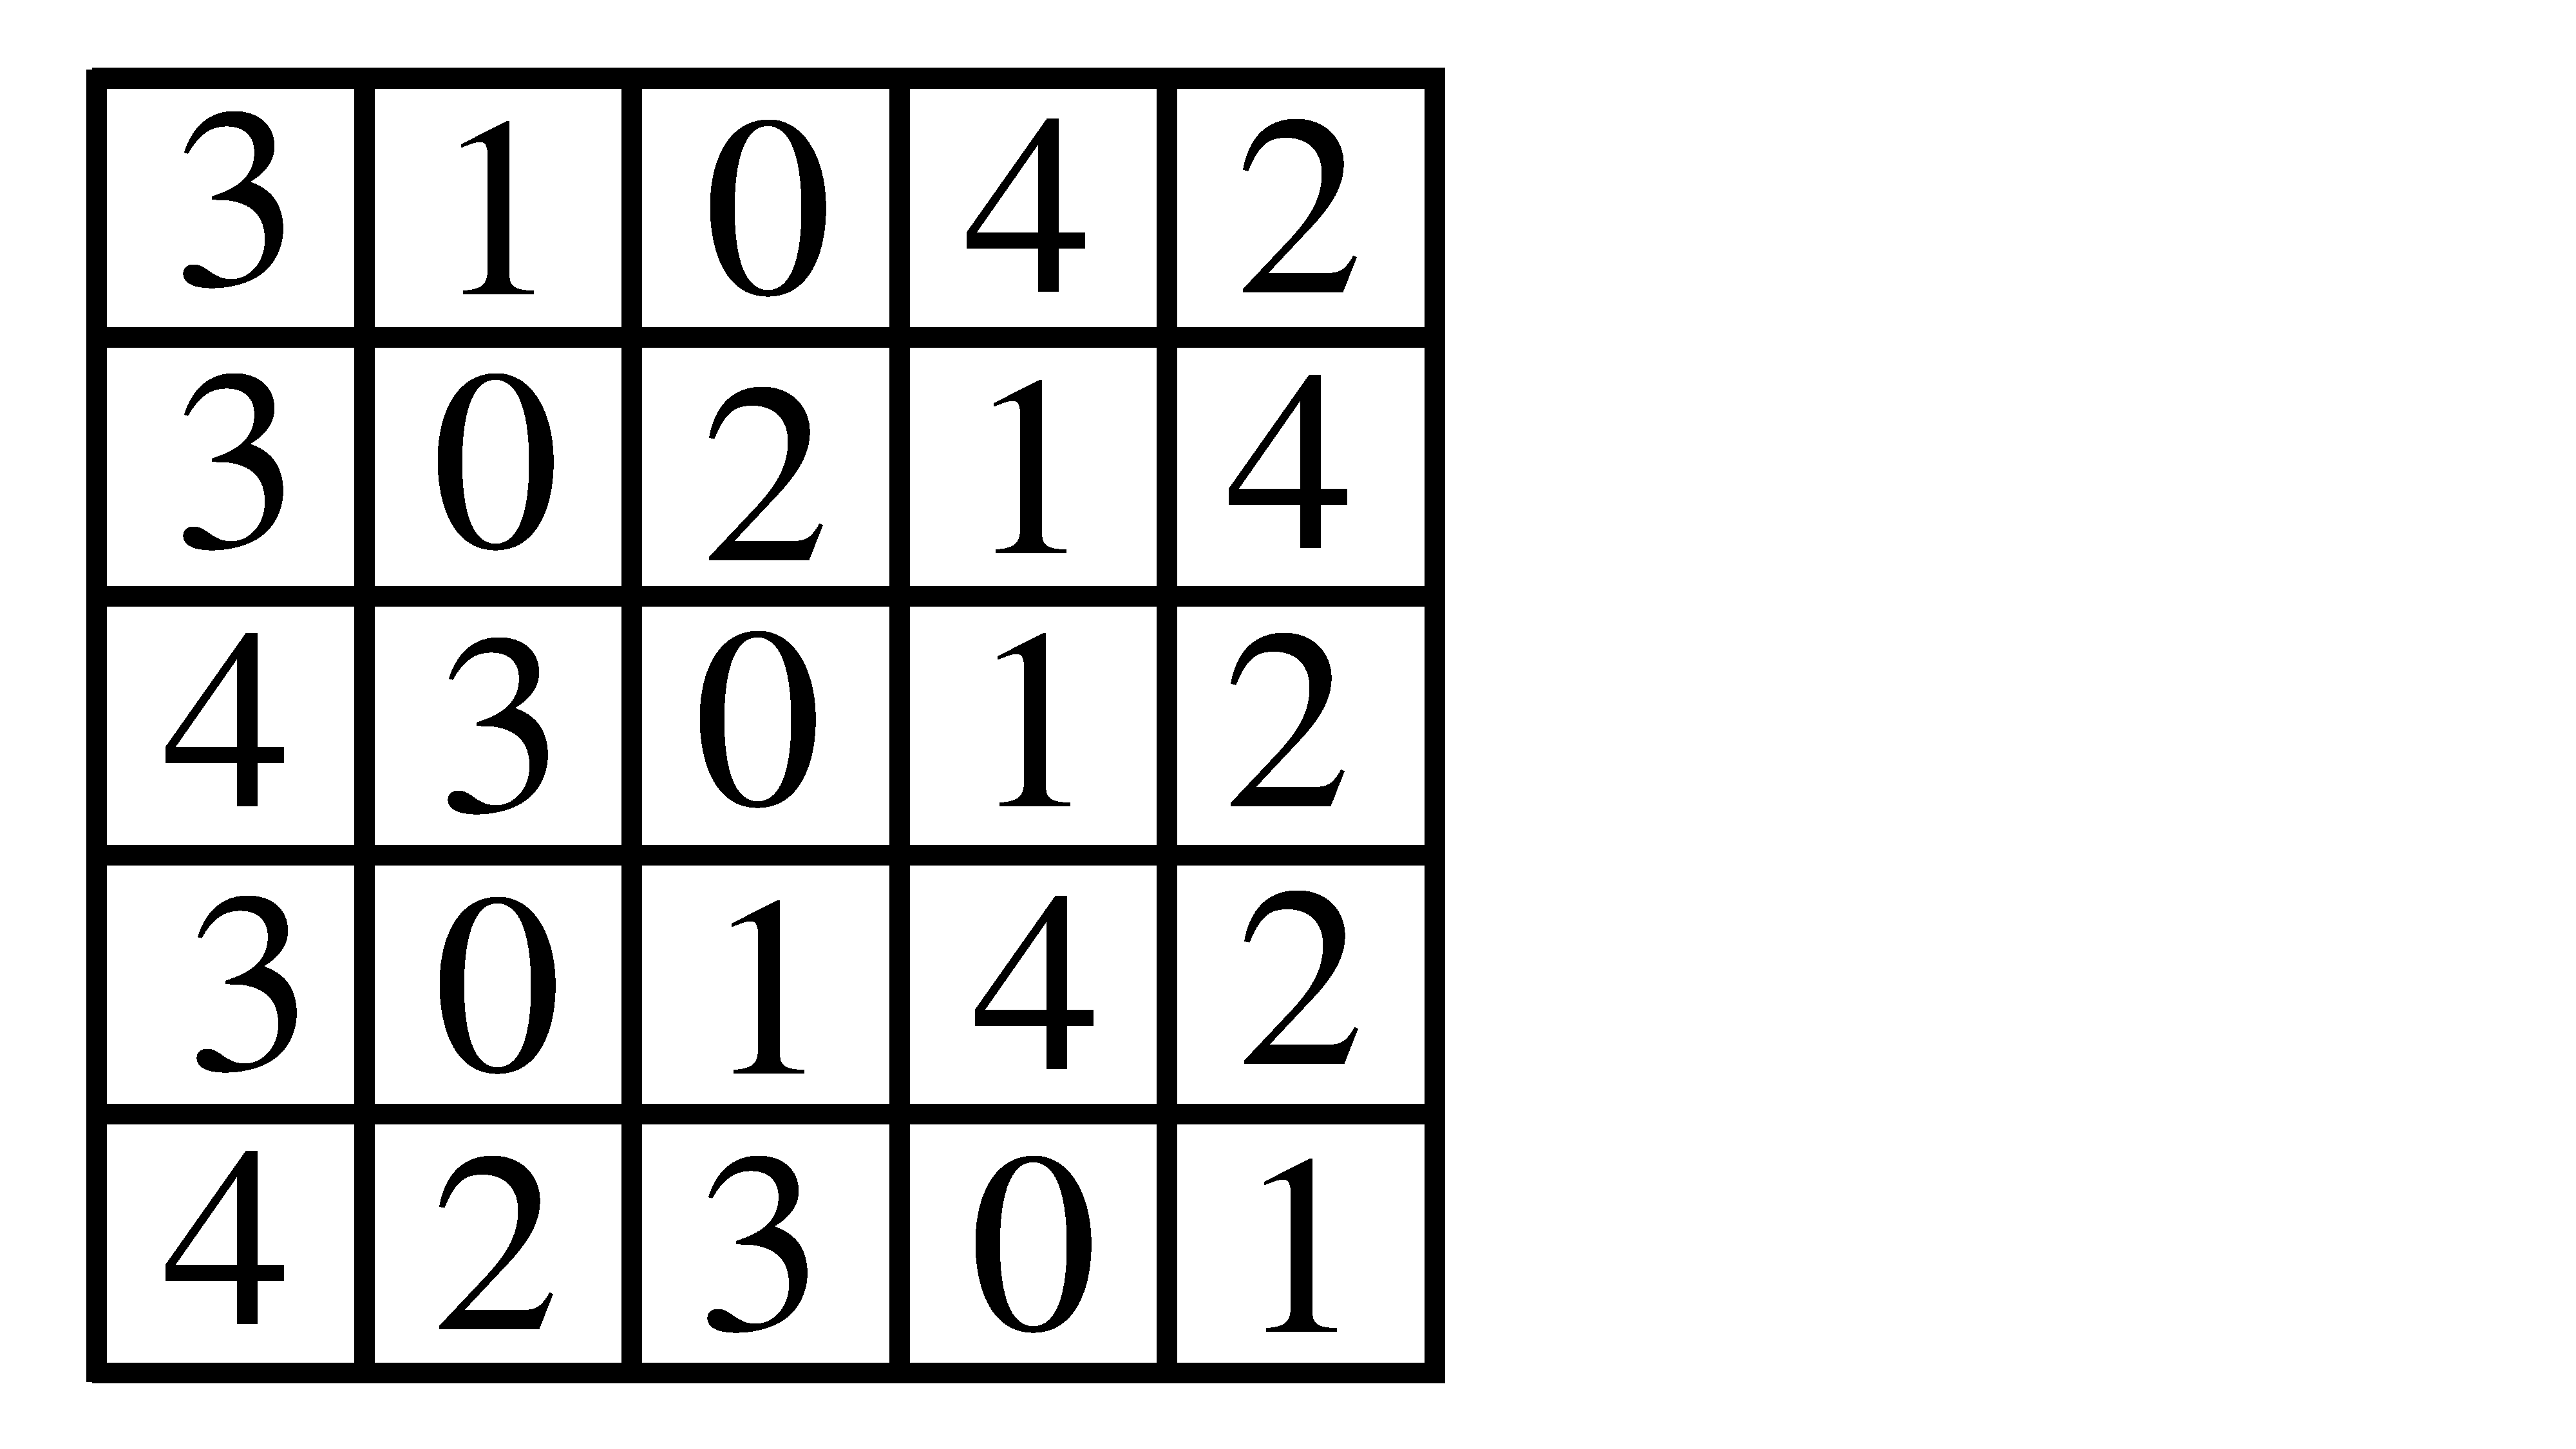
\includegraphics[width=\textwidth,trim=0mm 0mm 250mm 0mm, clip]{./figures/aMin1.pdf}
        \caption{Input $A$.}\label{sfig:aMin1}
    \end{subfigure} \hfill
       \begin{subfigure}[b]{0.15\textwidth}
        \centering
        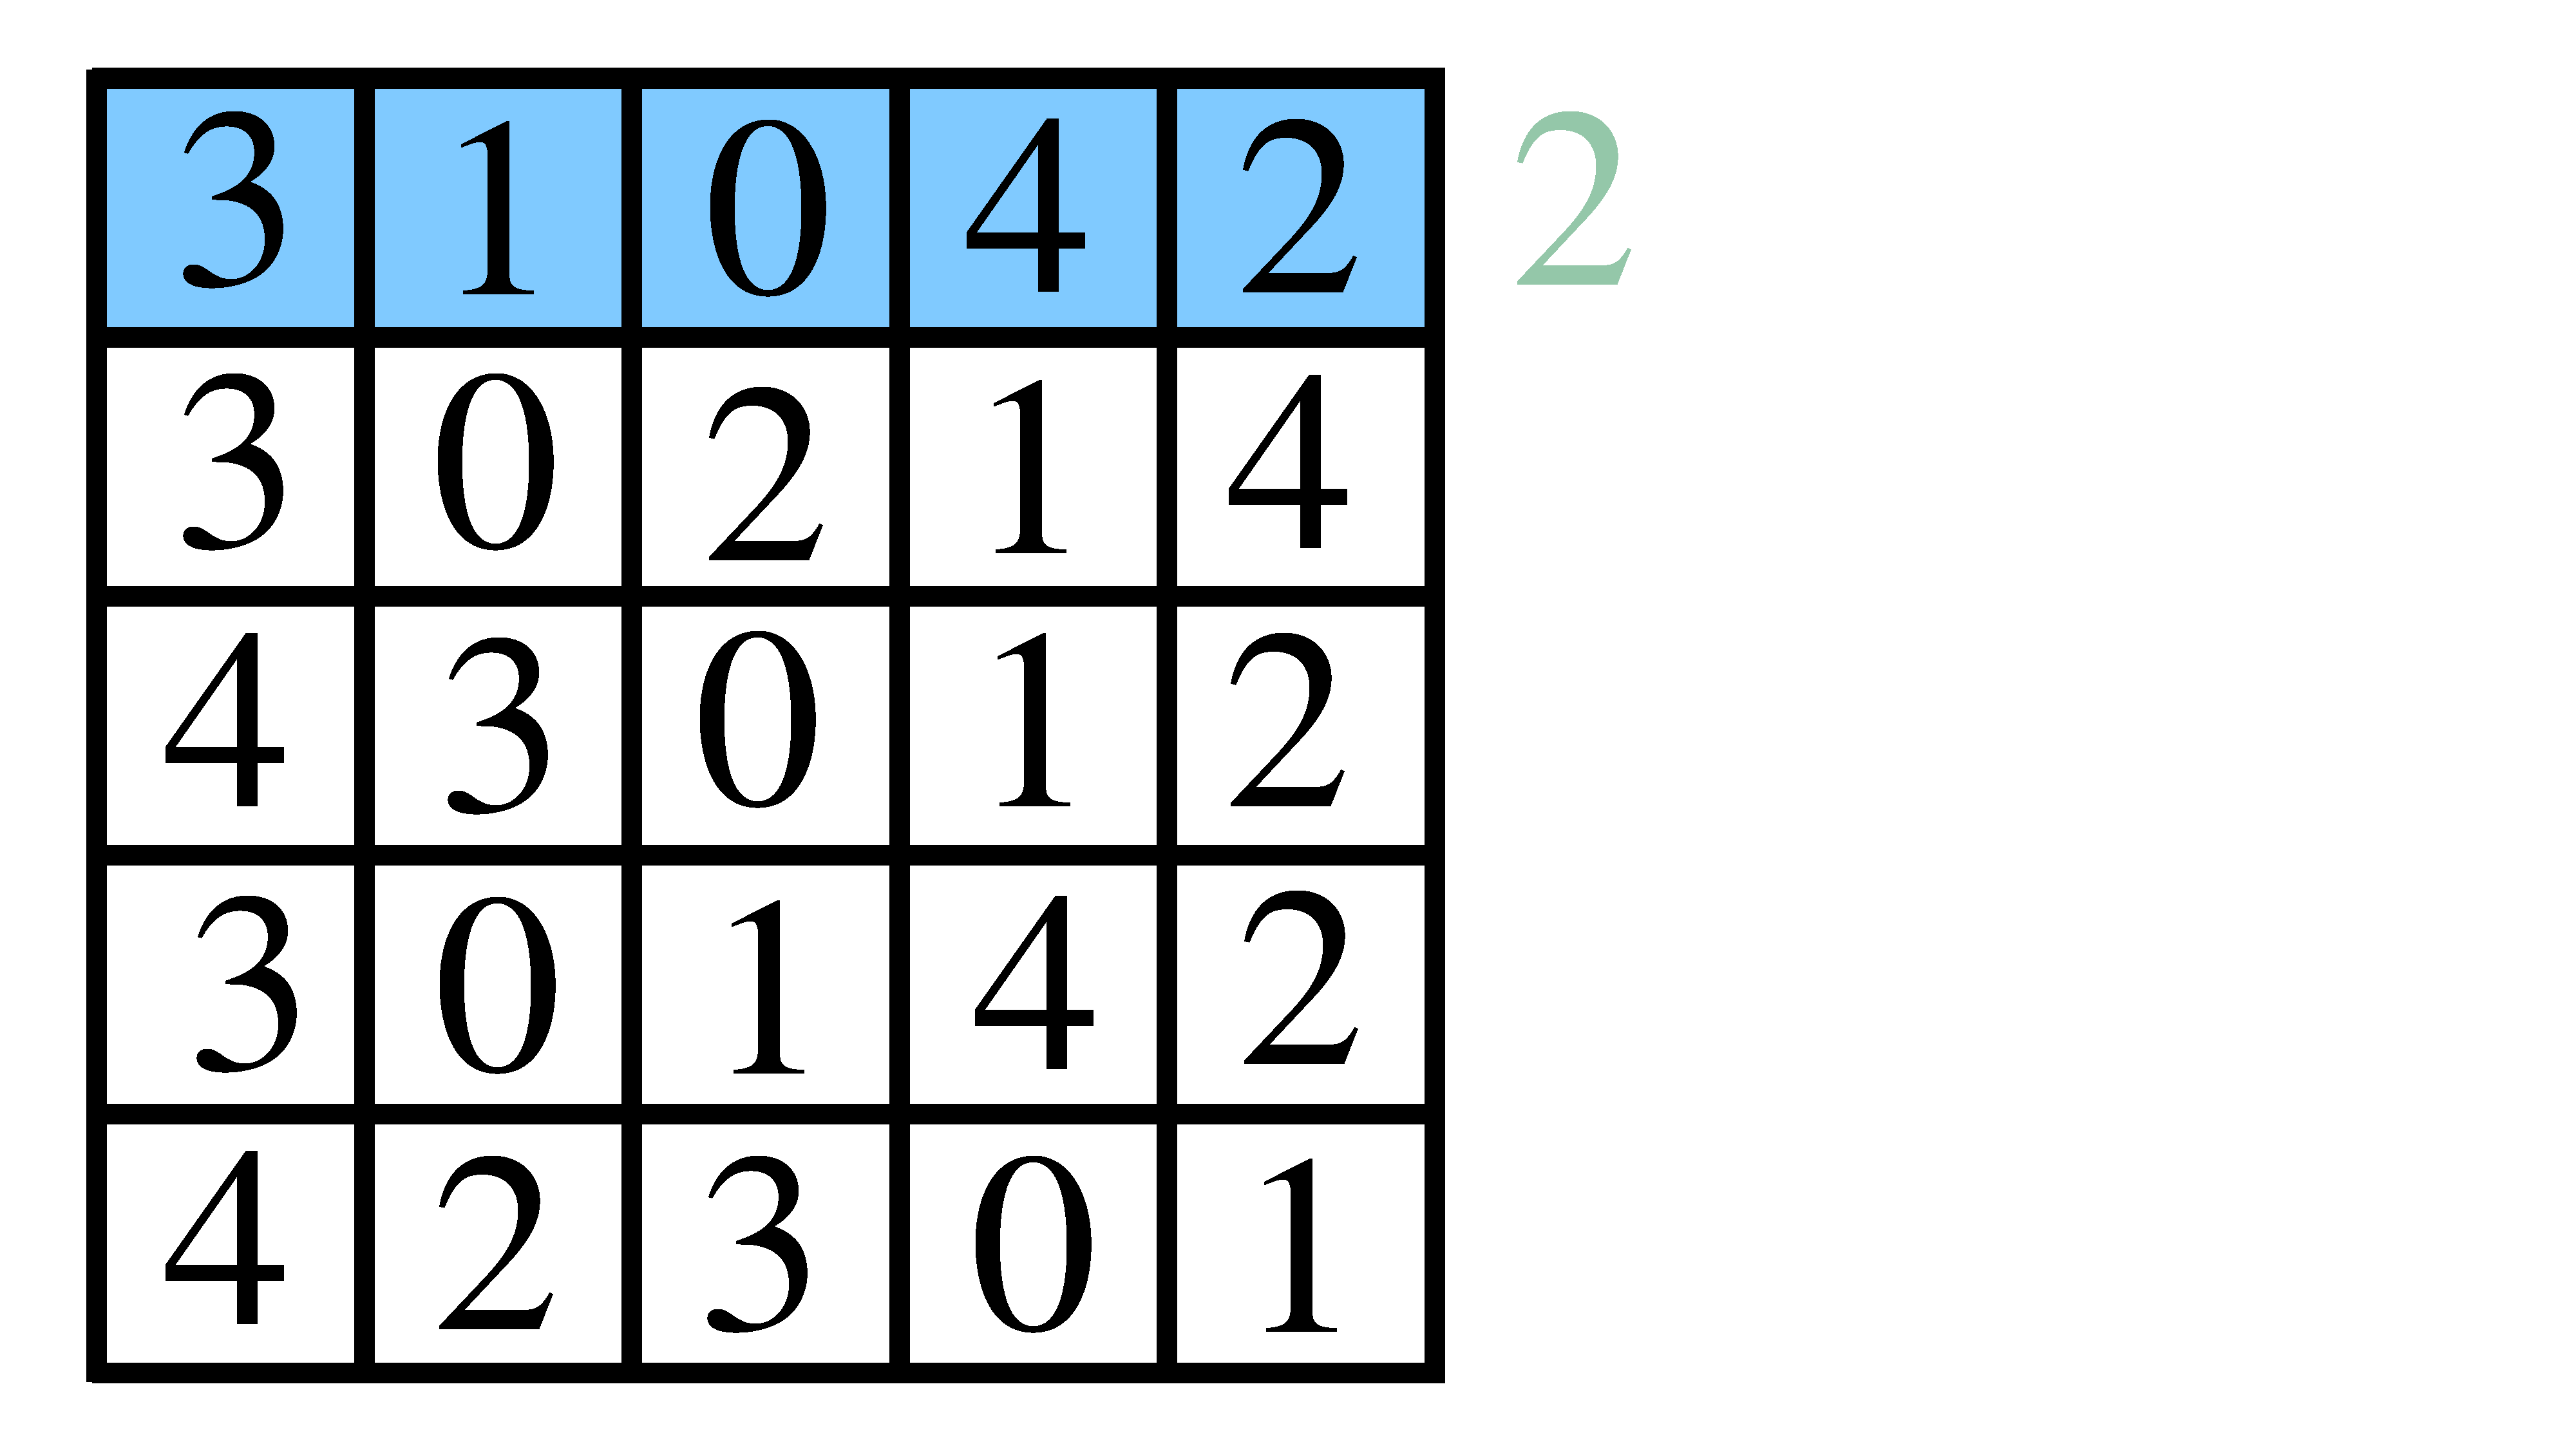
\includegraphics[width=\textwidth,trim=0mm 0mm 250mm 0mm, clip]{./figures/aMin2.pdf}
        \caption{Step $1$.}\label{sfig:aMin2}
    \end{subfigure} \hfill
       \begin{subfigure}[b]{0.15\textwidth}
        \centering
        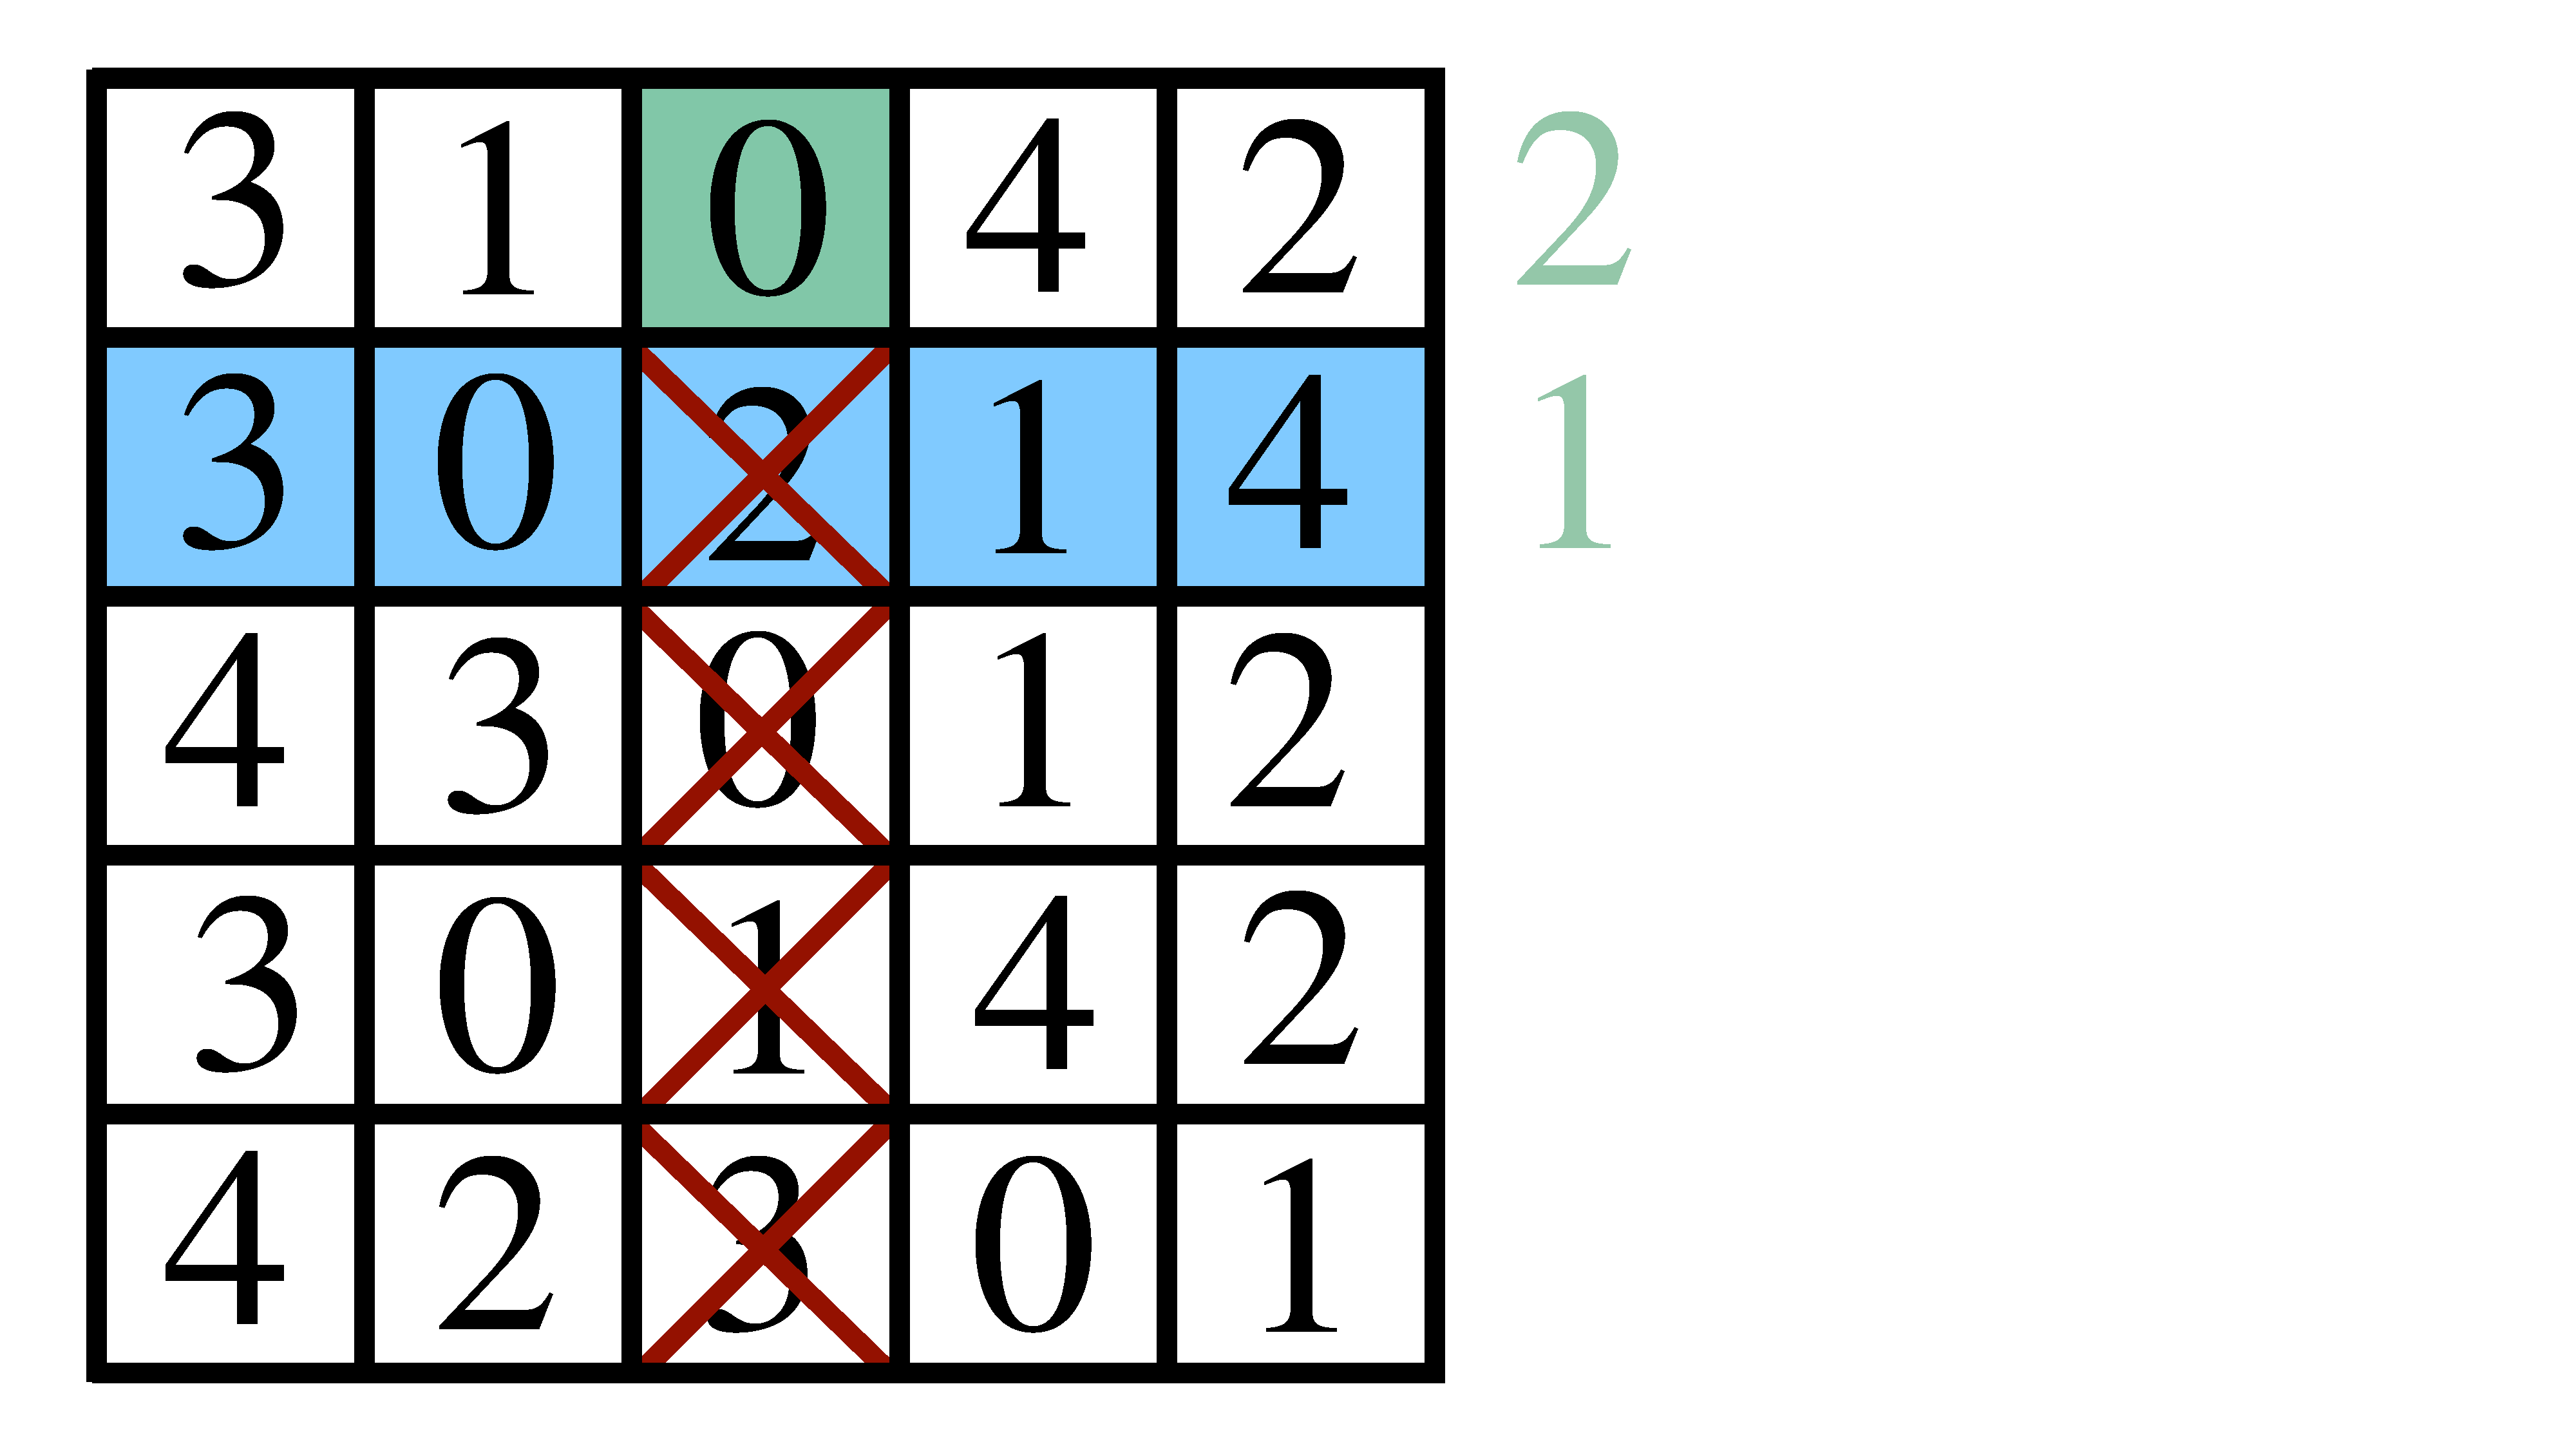
\includegraphics[width=\textwidth,trim=0mm 0mm 250mm 0mm, clip]{./figures/aMin3.pdf}
        \caption{Step $2$.}\label{sfig:aMin3}
    \end{subfigure} \hfill
    \begin{subfigure}[b]{0.15\textwidth}
        \centering
        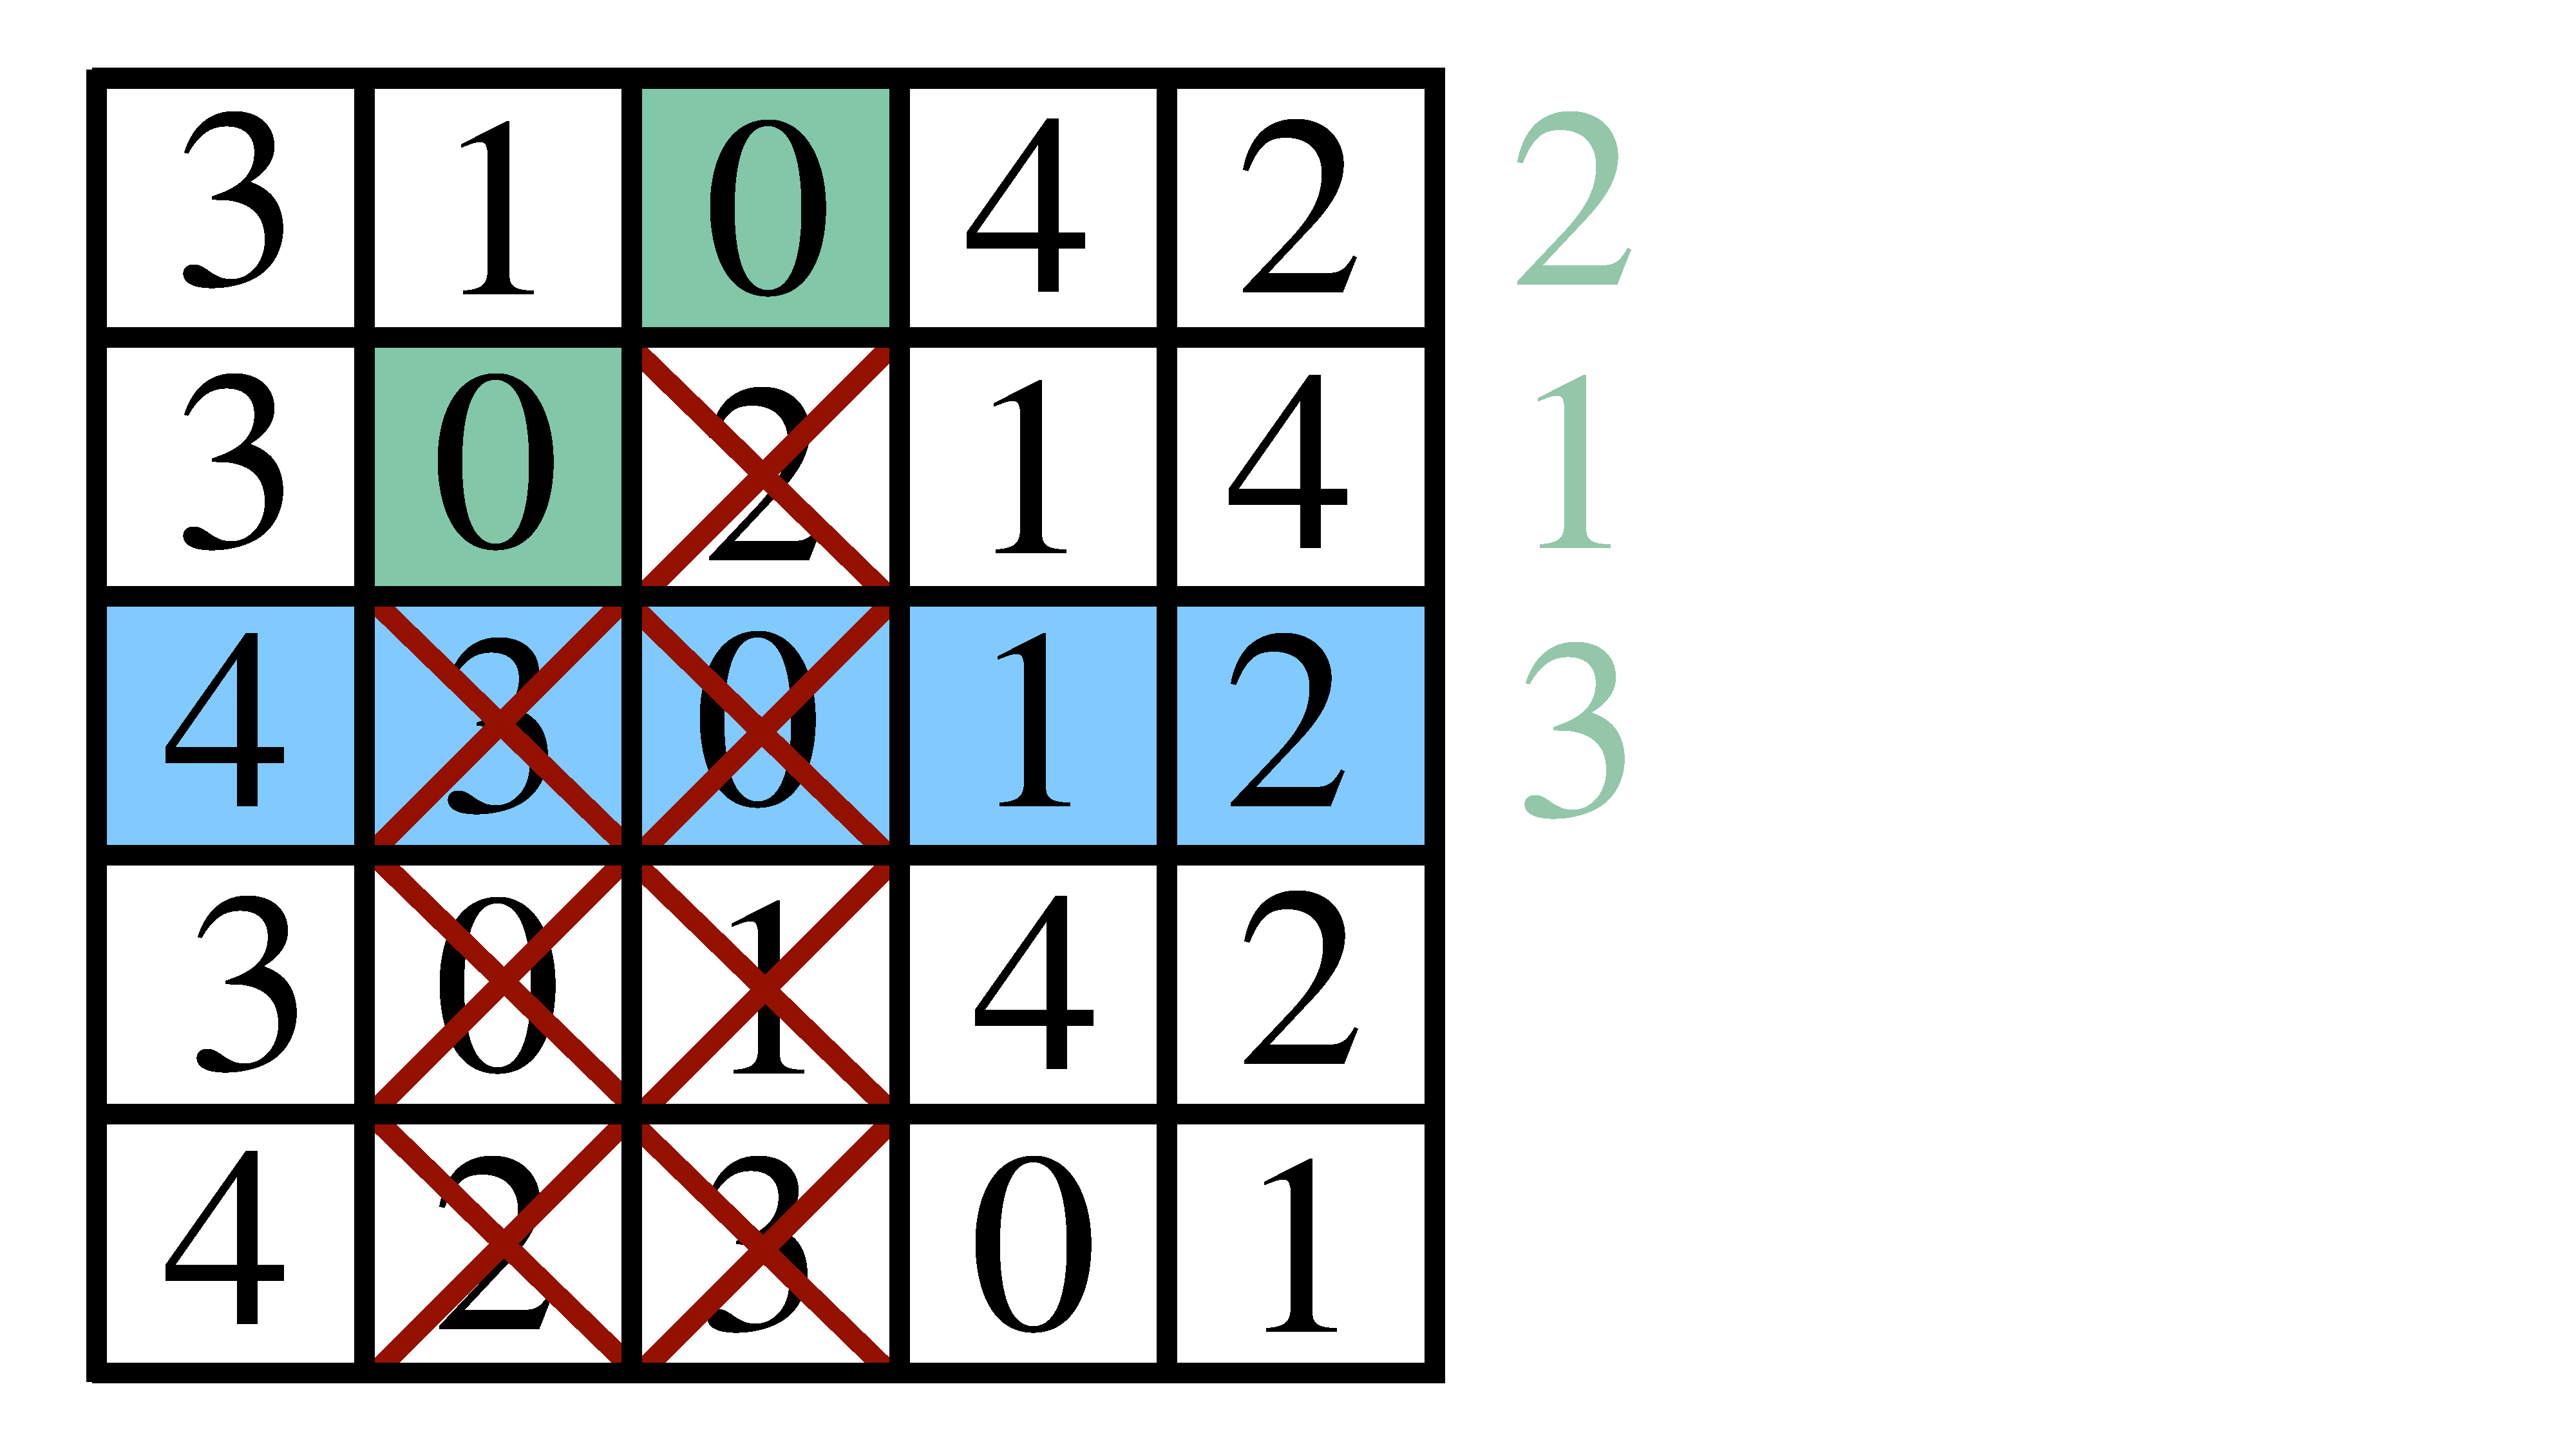
\includegraphics[width=\textwidth,trim=0mm 0mm 250mm 0mm, clip]{./figures/aMin4.pdf}
        \caption{Step $3$.}\label{sfig:aMin4}
    \end{subfigure} \hfill
    \begin{subfigure}[b]{0.15\textwidth}
        \centering
        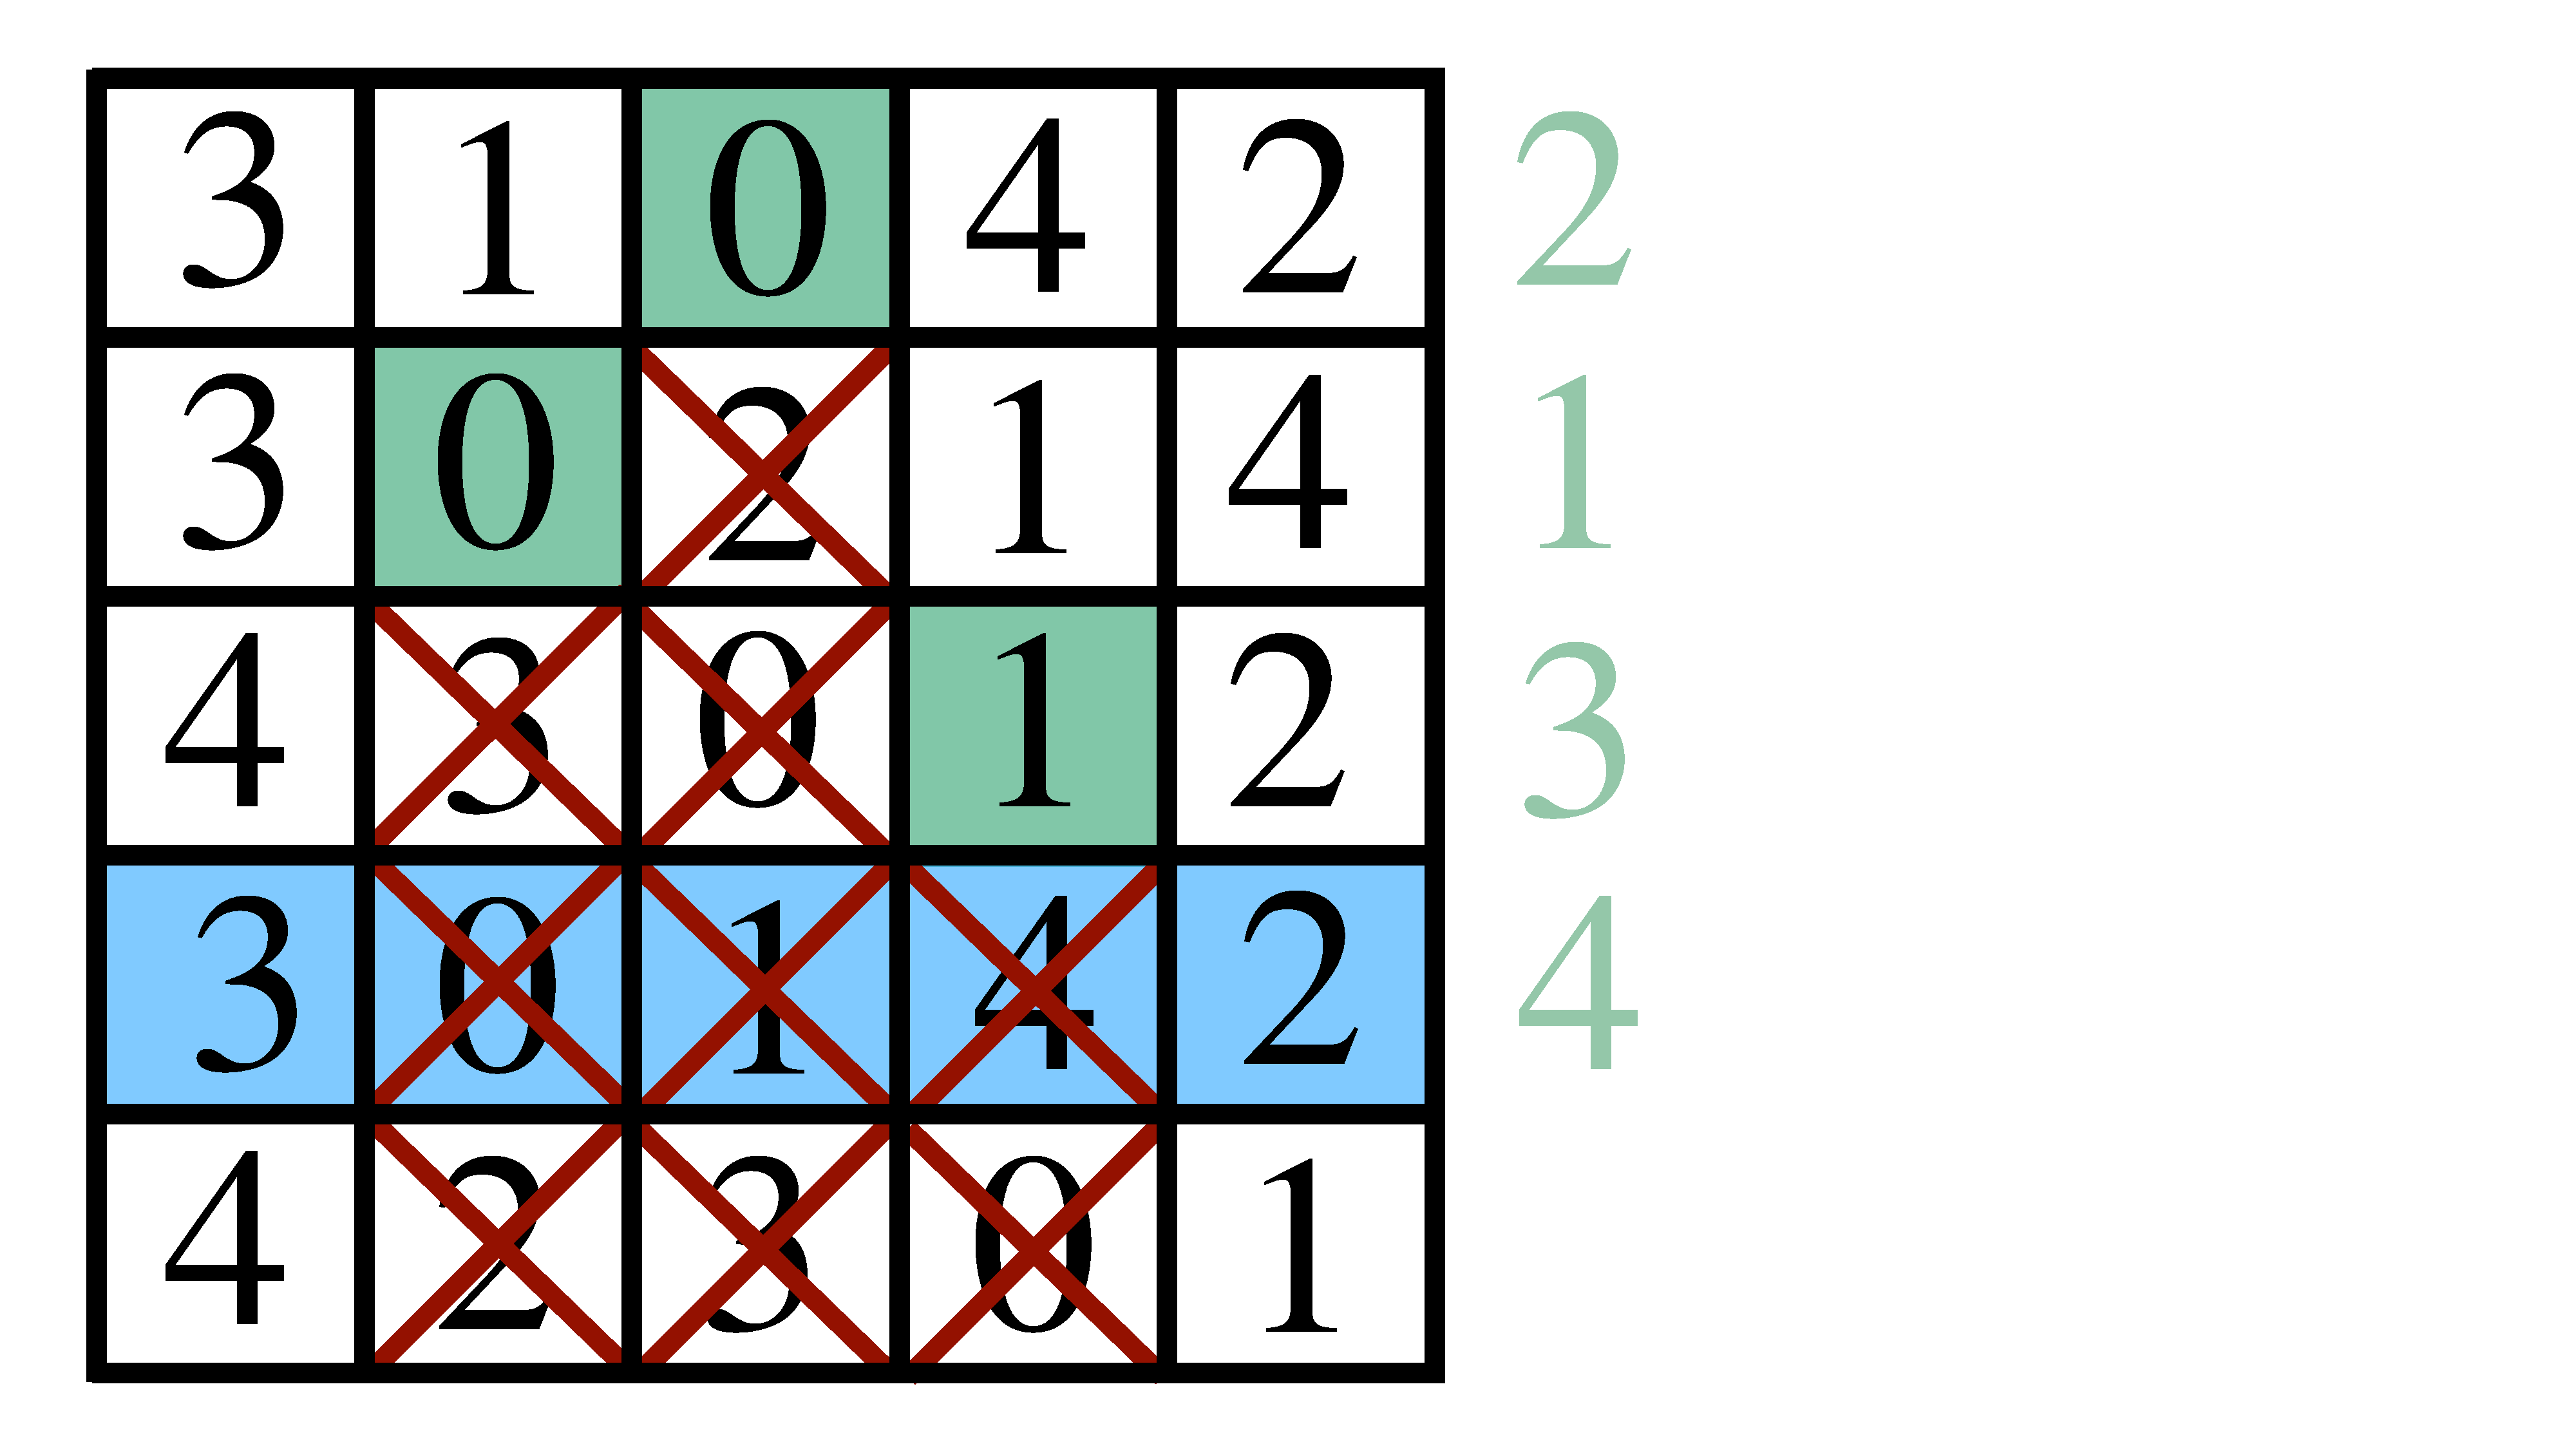
\includegraphics[width=\textwidth,trim=0mm 0mm 250mm 0mm, clip]{./figures/aMin5.pdf}
        \caption{Step $4$.}\label{sfig:aMin5}
    \end{subfigure} \hfill
    \begin{subfigure}[b]{0.15\textwidth}
        \centering
        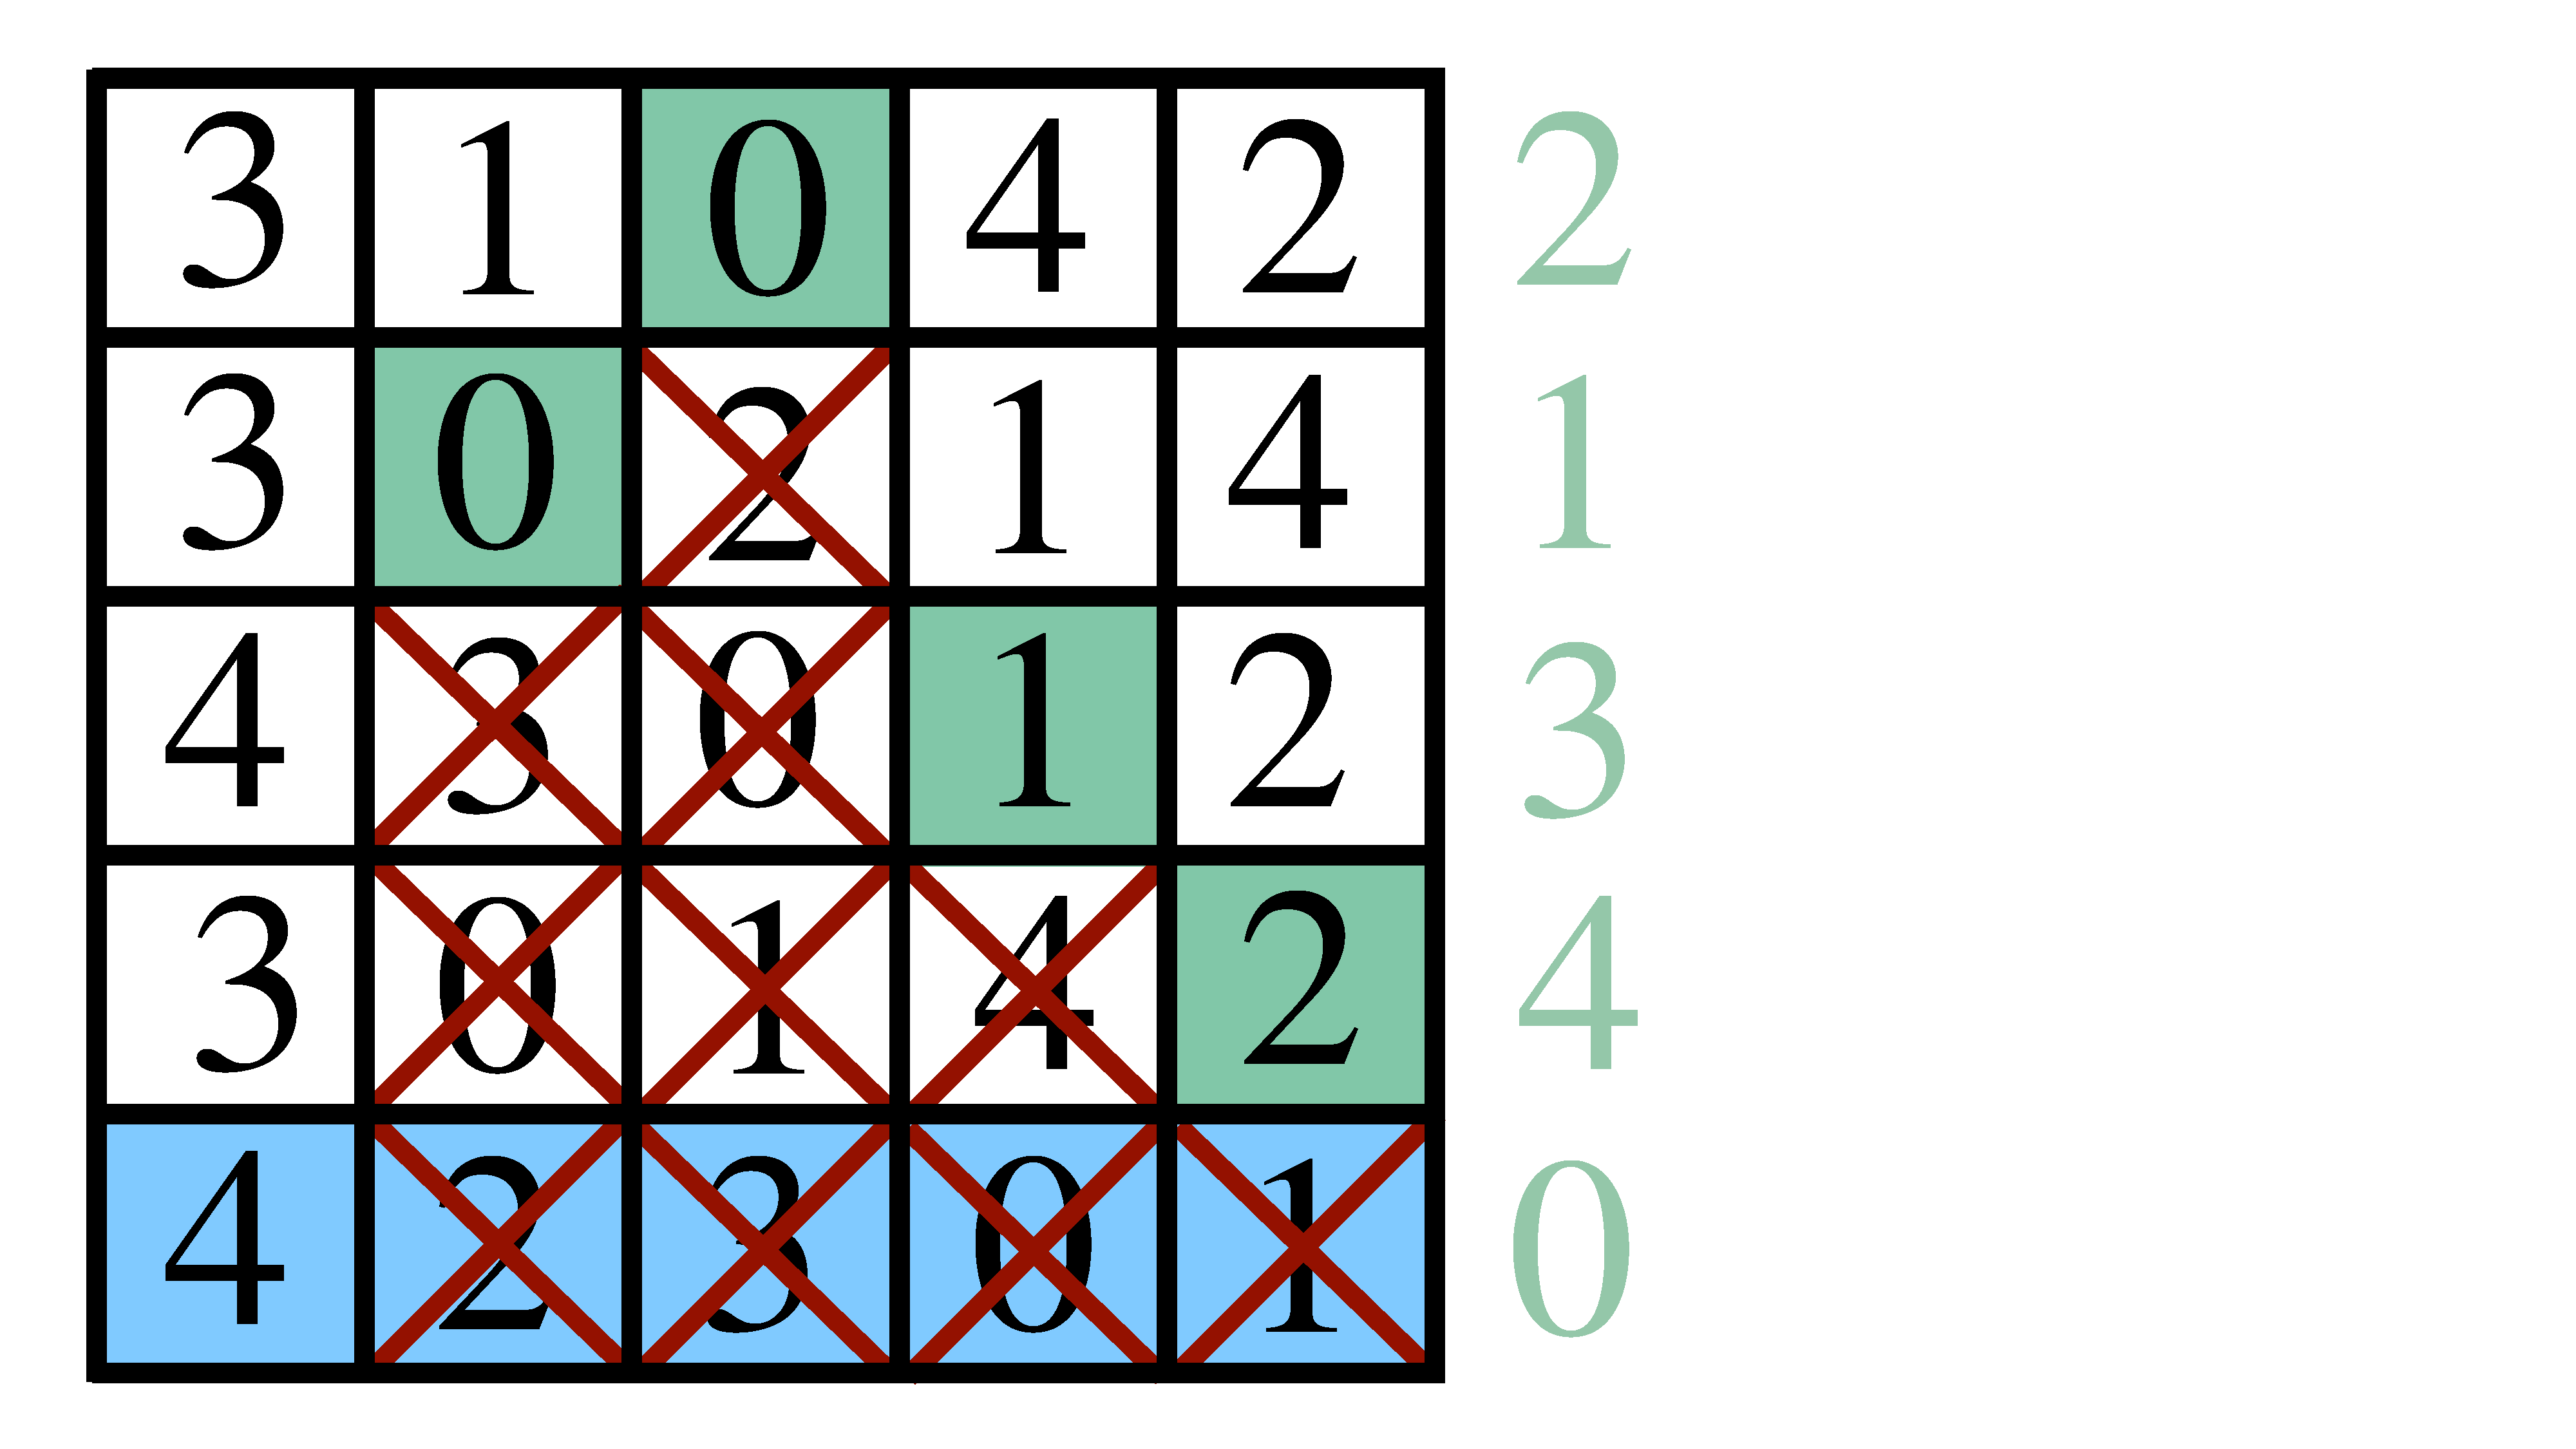
\includegraphics[width=\textwidth,trim=0mm 0mm 250mm 0mm, clip]{./figures/aMin6.pdf}
        \caption{Step $5$.}\label{sfig:aMin6}
    \end{subfigure} \hfill
    \caption{\am on matrix $A$. The row considered in each step is shown in blue. 
    $k_i$ for the $i$-th row written to the right of $A$ in green with witnessing entry of $A$ also in green. Indices removed from $I$ in relevant rows crossed out in red.} \label{fig:aMin}
\end{figure}



Observe that both problems \ref{prob:hac} and \ref{l:am} are defined as having an algorithm output an index $i \in \{1,2,\dots\}$. Thus, these can be considered search problems instead of decision problems. We choose to work with the search versions of these problems for simplicity of our reductions, however, our reduction naturally extends to the decision variants  (e.g., where the algorithm is given $u,v \in V$ and an index $i$ and asked if $u,v$ merge on step $i$). 

We first prove the \CC-hardness of this intermediate problem. See \Cref{fig:aMinRed} for an illustration of our reduction from \lfm to \am.
\begin{lemma}
\am is \CC-hard.
\end{lemma}
\begin{proof}
    By \Cref{thm:LFMCCComplete} and the definition of \CC-hardness (\Cref{dfn:CCComplete}), it suffices to argue that \lfm (\Cref{dfn:LFMM}) is logspace reducible to \am (\Cref{l:am}).
    % \kgnote{Shouldn't this be the other way?}\rnote{agreed, I switched it}. 
    We begin by describing our reduction and then observe that it only requires logarithmic space. The basic idea of the reduction is to associate with each vertex on the left side of our instance of \lfm a row of the matrix of \am and each vertex on the right side of \lfm a column of the matrix of \am.

    More formally, consider an instance of \lfm on graph $G = (V = L \sqcup R, E)$ where our goal is to decide if a given edge $e$ is in the LFM matching. 
    % Let $n := \max\{|L|, |R|\}$.
    % \hnote{At least in the Cook-Filmus-Le paper, left and right have the same size, so we don't need to bother about this.}
    We consider the following instance of \am to solve this on a $2n \times 2n$ size matrix $A$. We will refer to an index $i$ as a \emph{dummy index} if $i \geq n$. We will construct the $i$th row of $A$ to correspond to a permutation that first gives the indices of all neighbors of $l_i$ in $R$ sorted according to the ordering of $R$ then gives all dummy indices then gives the indices of non-neighbors of $l_i$ in $R$. 
    
    More formally, for a vertex $l_i \in L$, we let $R_i \subseteq R$ be the vertices of $G$ connected to $l_i$ and we let $\bar{R_i} = R \setminus R_i$ be all vertices not adjacent to $l_i$. Furthermore, for $r_j \in R_i$, we let $\text{ind}(r_j) \in [|R_i|]$ be the index of $r_j$ in $R_i$ when we sort the vertices of $R_i$ according to the ordering on $R$. Note that, in general, it need not be the case that $\text{ind}(r_j) = j$. Symmetrically, for a vertex $r_j \in \bar{R_i}$, we let $\text{ind}(r_j) \in [|\bar{R_i}|]$ be the index of $r_j$ when we sort $\bar{R_i}$ by the ordering on $R$. Then, we define $A$ as follows.
    \begin{align*}
        A[i,j] := \begin{cases} \text{ind}(r_j) &\text{if $j < n$ and $r_j \in R_i$}\\
        j - n + |R_i| & \text{if $j \geq n$}\\
        \text{ind}(r_j) + n + |R_i|  & \text{if $j < n$ and $r_j \not \in R_i$}
        \end{cases}
    \end{align*}
    
    
    % Specifically, the first $|R_i|$ indices of $\pi_i$ will be the indices of $R_i$ (sorted by their order in $R$), the next $n$ indices will be dummy indices $n, n+1, \ldots 2n-1$ and the remaining $n- |R_i|$ indices will be the indices of vertices in $R \setminus R_i$ (sorted, say, by their order in $R$).
    % More formally, we say that a permutation $\pi$ of $[2n]$ is consistent with $l_j$ if for each $i$ such that $r_i \in R_j$ we have that $i$ precedes $i'$ in $\pi$ if
    % \begin{itemize}
    %     \item $r_{i'} \in R_j$ but $i < i'$ or
    %     \item $i'$ is a dummy index or
    %     \item $r_{i'} \not \in R_j$
    % \end{itemize}
    % and for each $i$ which is a dummy index we have that $i$ precedes $i'$ in $\pi$ if $r_{i'} \not \in R_j$. Then, let the $j$th row of $A$ be any permutation of $[2n]$ consistent with $l_j$. 
    % For $i \geq n$ we can construct our permutation arbitrarily. 
    Lastly, let $x$ (the index for which we would like to compute $k_x$ in our instance of \am) be the index of the endpoint of $e$ in $L$.
    % \hnote{Added note about mapping the results back.}
    Once \am computes $k_x$, we verify whether or not it corresponds to the endpoint of $e$ in $R$ to determine the final output of the \lfm instance. Again, see \Cref{fig:aMinRed}.

    % \hnote{We should be careful about saying ``in the $j$th round,'' and rather say ``at the beginning of the round.''}
    % \enote{I'm using notation that needs to be defined above where $i_j := \argmin_{i \in I} A[j, i]$ in the $j$th round of the \am algorithm.}
    We now argue correctness of the reduction. A straightforward proof by induction on $i$ demonstrates that at the beginning of the $i$th round of the \am algorithm we have that $I$ consists of at least $n-i$ dummy indices and $j < n$ is not in $I$ only if $r_j$ is in the \lfm and is matched to some $l_{i'}$ for $i' < i$. It follows that $e = (l_i, r_j)$ is in the \lfm iff $k_i = j$, showing correctness of our reduction. %\enote{Check the API for \am once it is maybe updated to make sure this makes sense.}

    It remains to show that the above reduction can be done with logspace. In order to do so, we must argue that $A[i,j]$ can be computed with logspace for every $i$ and $j$. Doing so is trivial given the above definition of $A[i,j]$. 
    % if $i$ is a dummy index, so consider $i < n$.
    % \begin{itemize}
    %     \item If $j \leq |R_i|$ then $A[i,j]$ is just the index of the $j$th vertex of $R_i$ (i.e., neighbor of $l_i$) in the ordering given by $R$.
    %     \item If $j \in [|R_i|, |R_i|+n]$ then $A[i,j]$ just is $j-|R_j| + n$.
    %     \item If $j > |R_i|+n$ then $A[i,j]$ is the index of the $(j - |R_i|-n)$th vertex in $R \setminus R_i$ (i.e., non-neighbors of $l_i$) when vertices of $R \setminus R_i$ are sorted according to the ordering on $R$.
    % \end{itemize}
    % All three of the above quantities can easily be computed in logspace.
\end{proof}

\begin{figure}[h]
    \centering
    \begin{subfigure}[b]{0.24\textwidth}
        \centering
    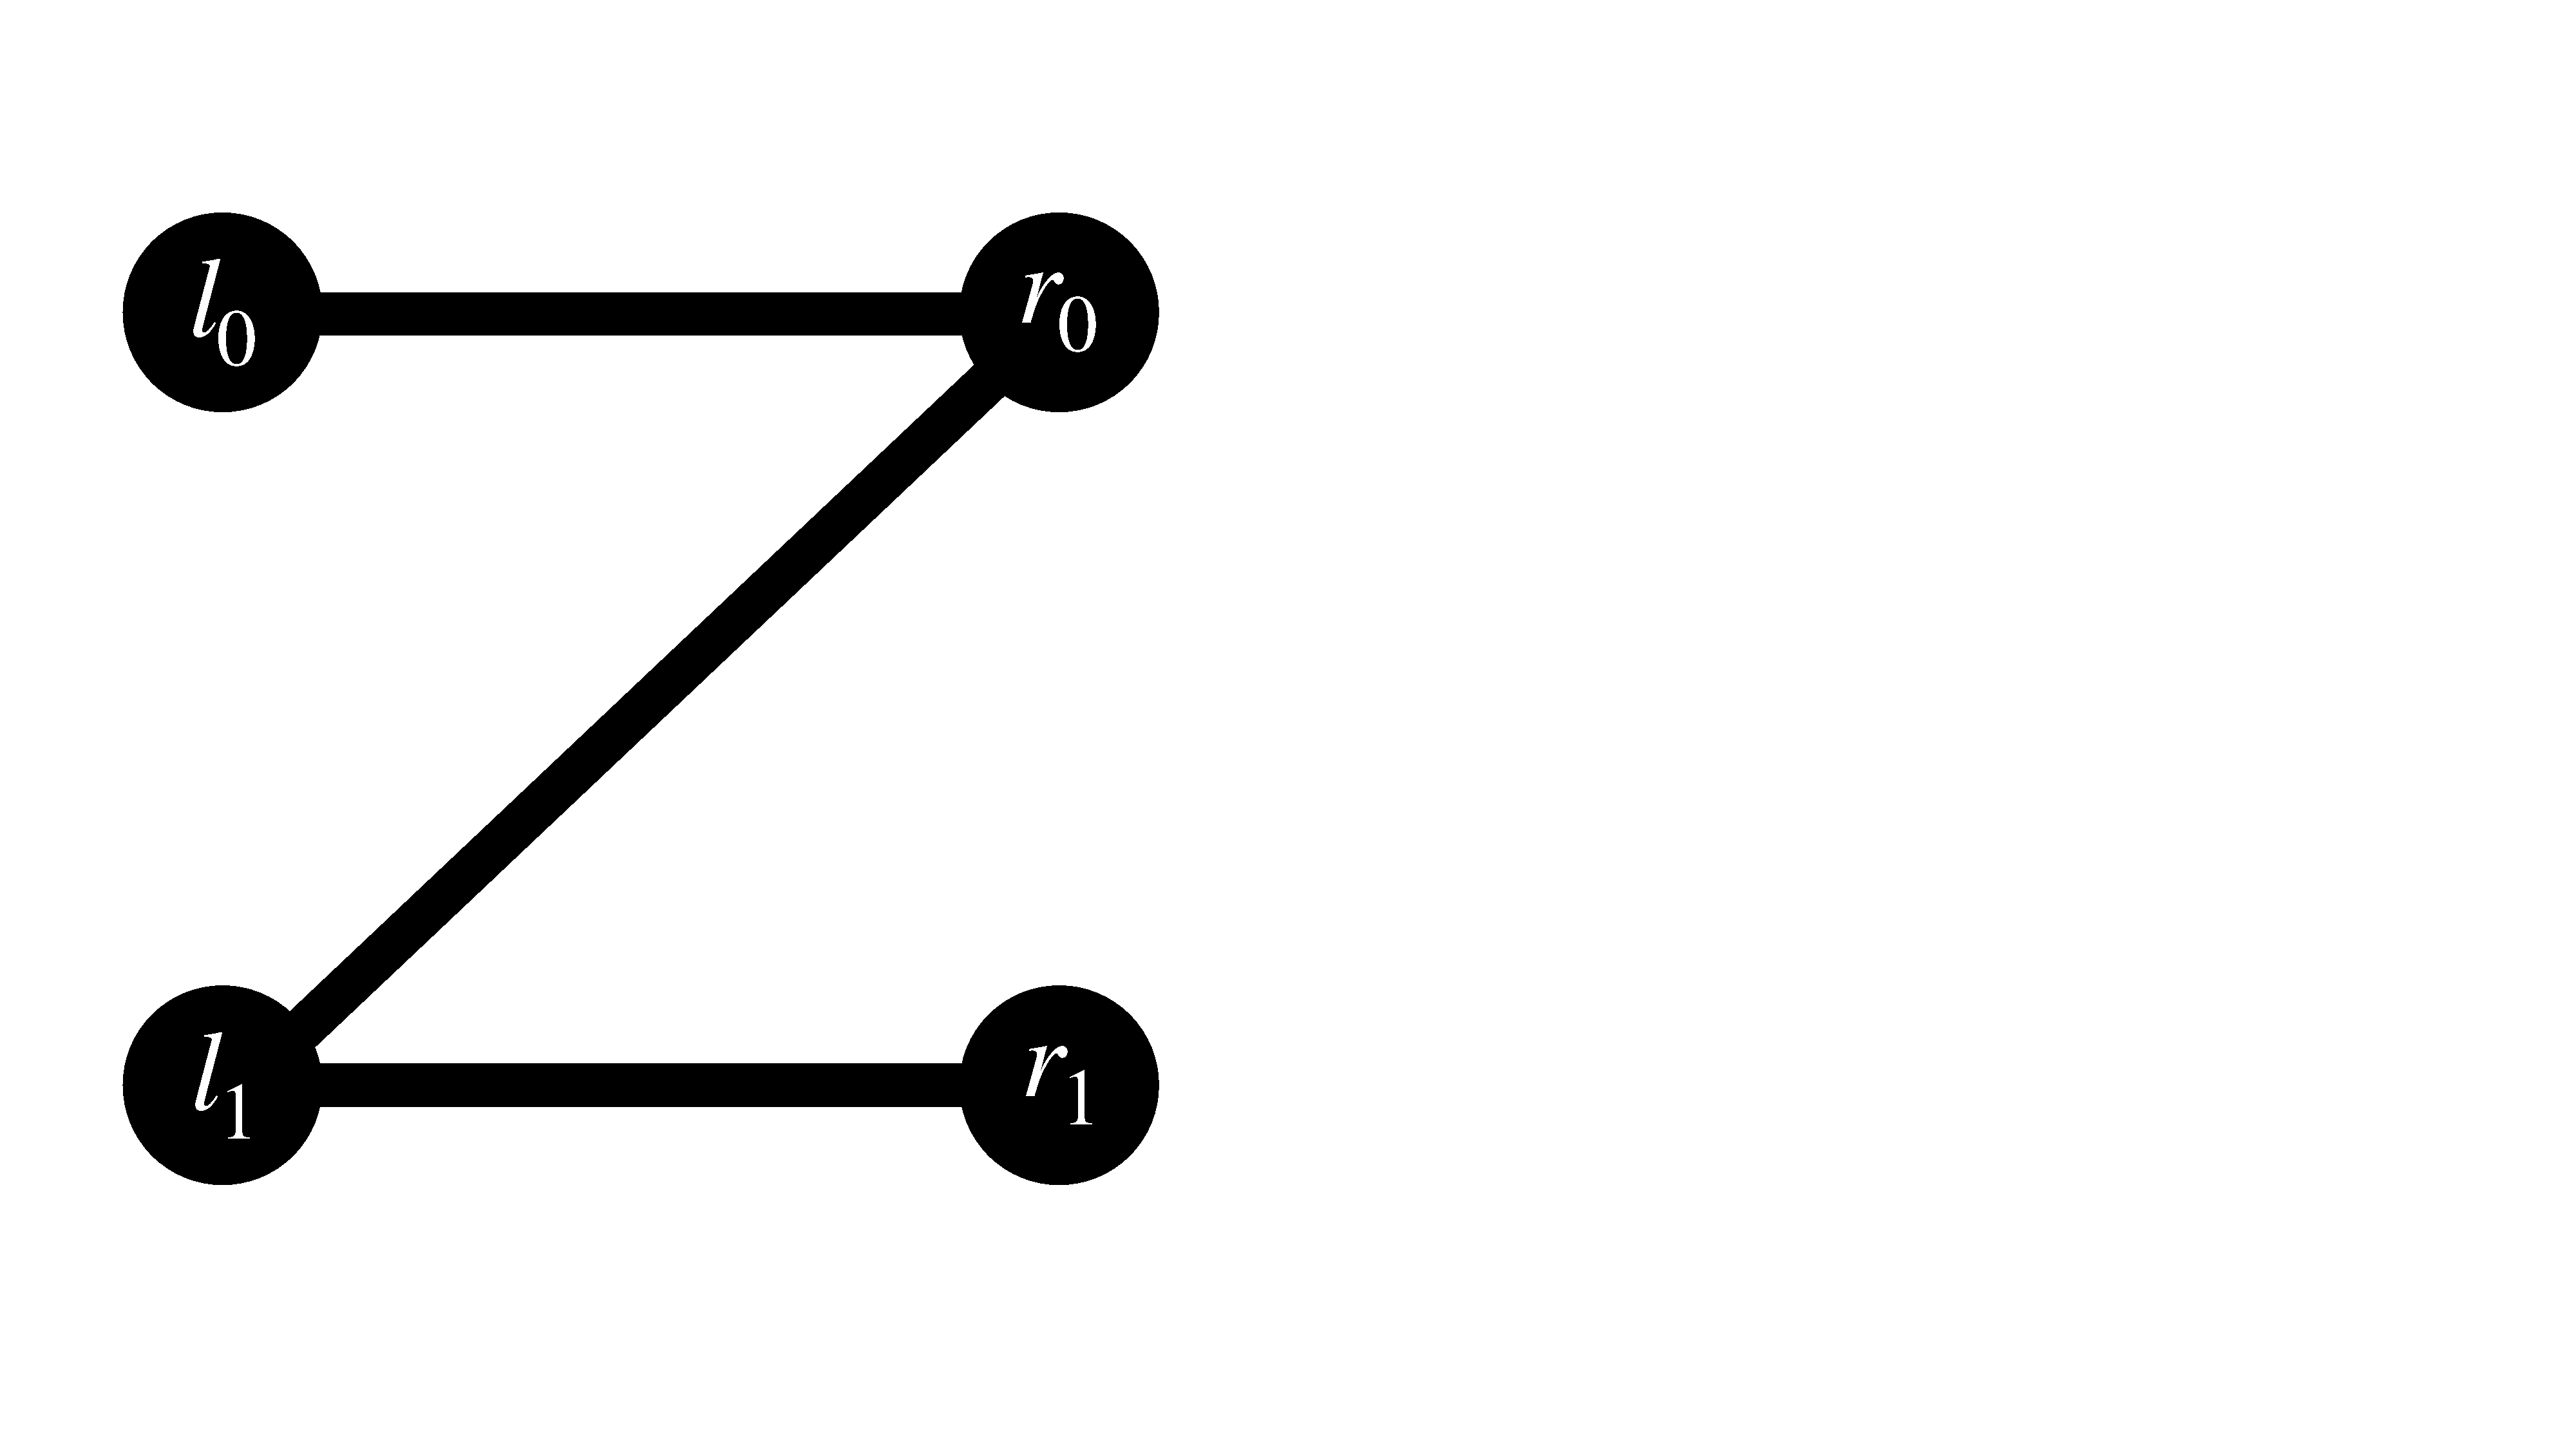
\includegraphics[width=\textwidth,trim=0mm 50mm 350mm 0mm, clip]{./figures/aMinRed1.pdf}
        \caption{\lfm.}\label{sfig:aMinRed1}
    \end{subfigure} \hfill
       \begin{subfigure}[b]{0.24\textwidth}
        \centering
    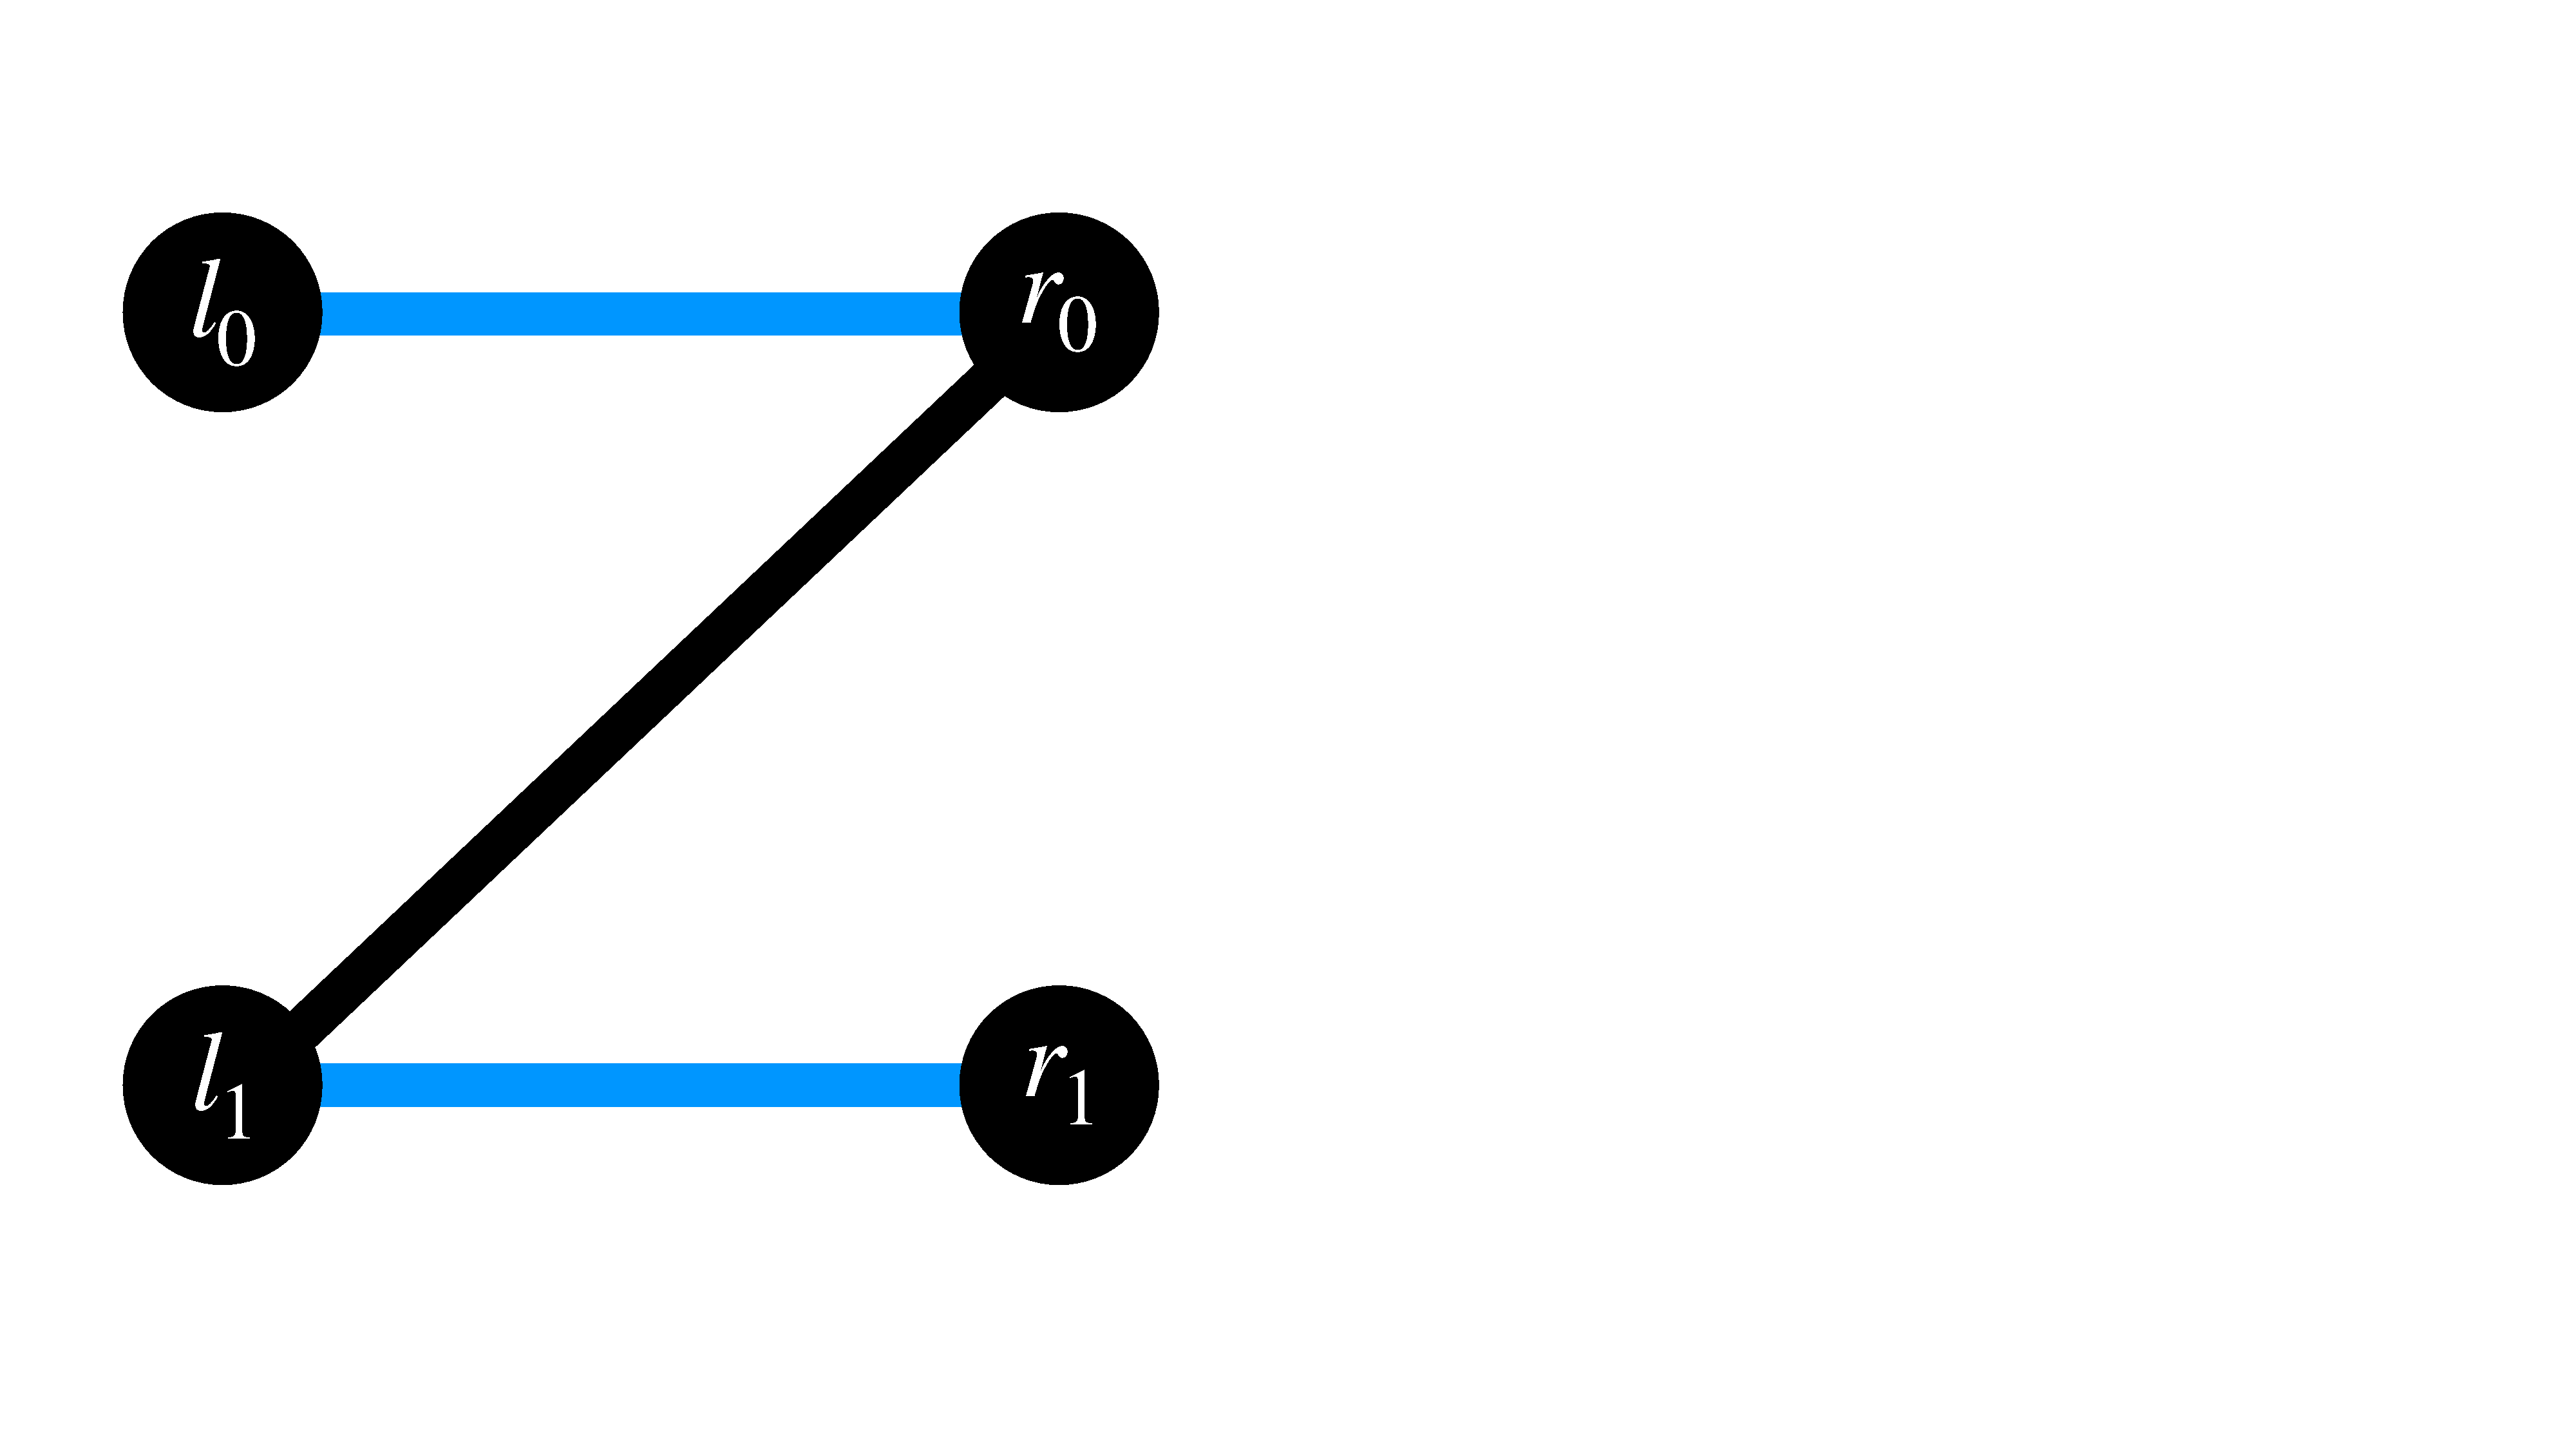
\includegraphics[width=\textwidth,trim=0mm 50mm 350mm 0mm, clip]{./figures/aMinRed2.pdf}
        \caption{Solution.}\label{sfig:aMinRed2}
    \end{subfigure} \hfill
       \begin{subfigure}[b]{0.24\textwidth}
        \centering
    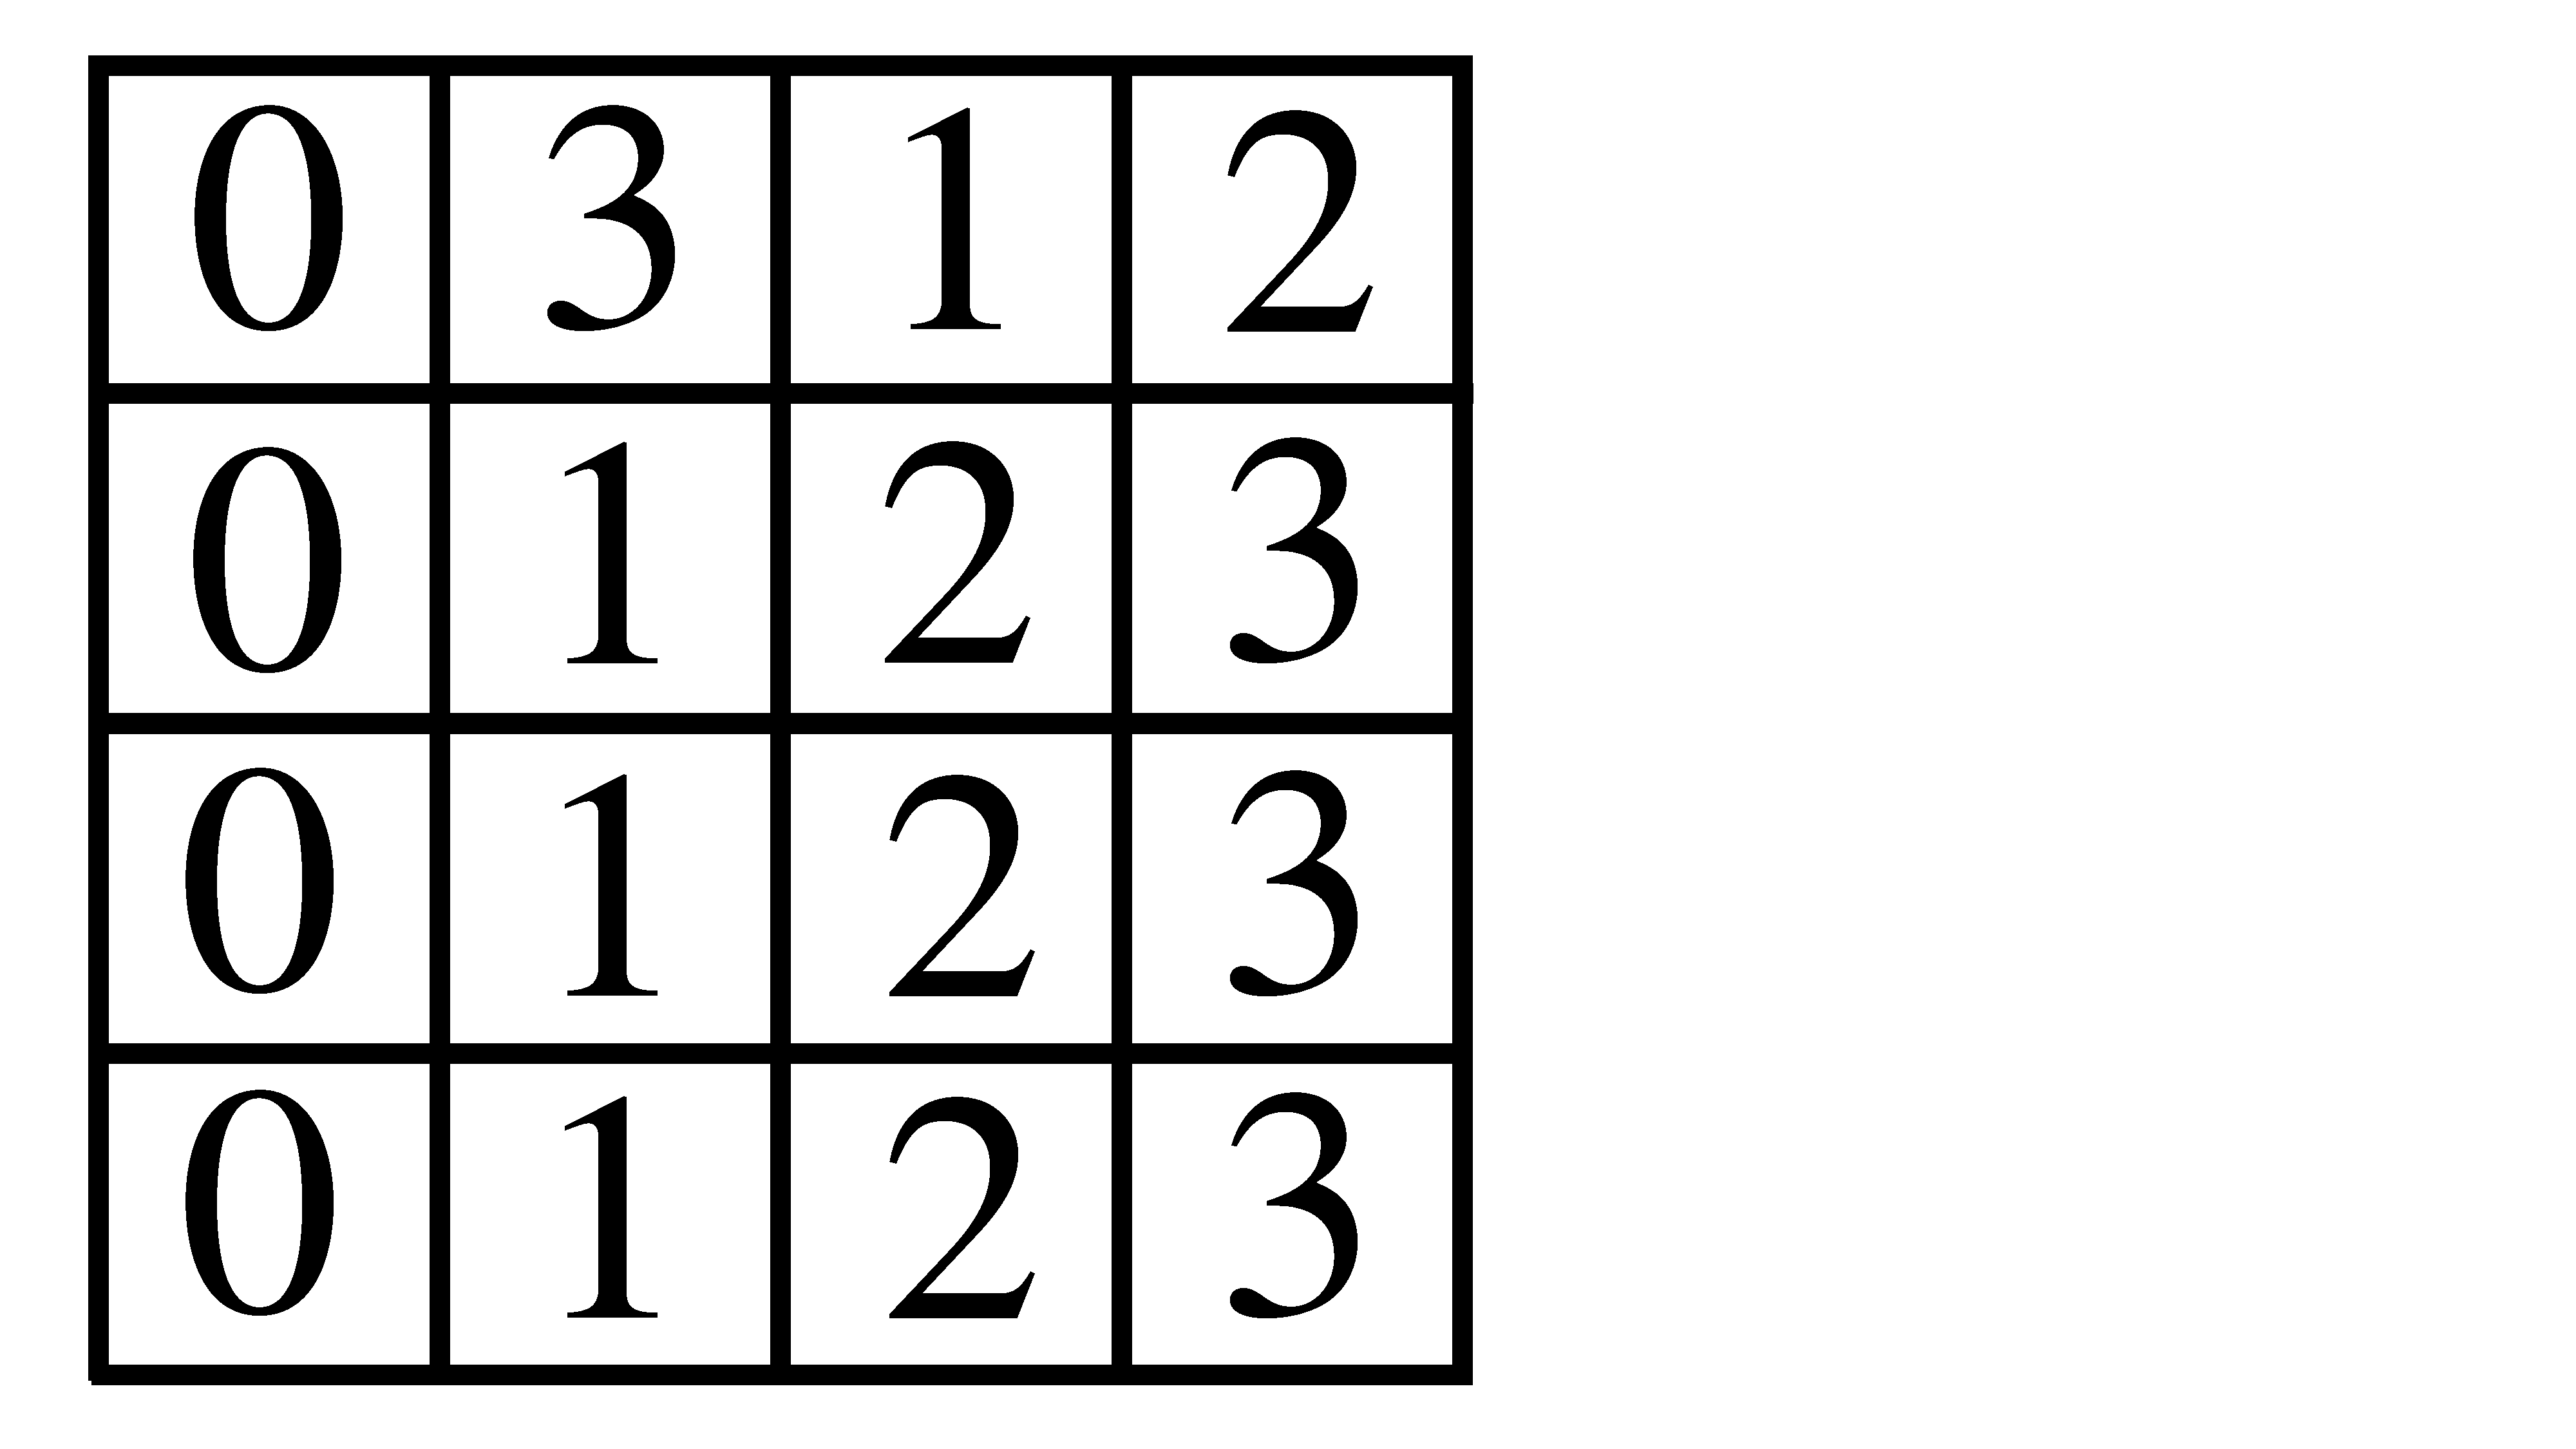
\includegraphics[width=\textwidth,trim=0mm 0mm 230mm 0mm, clip]{./figures/aMinRed3.pdf}
        \caption{\am.}\label{sfig:aMinRed3}
    \end{subfigure} \hfill
    \begin{subfigure}[b]{0.24\textwidth}
        \centering
        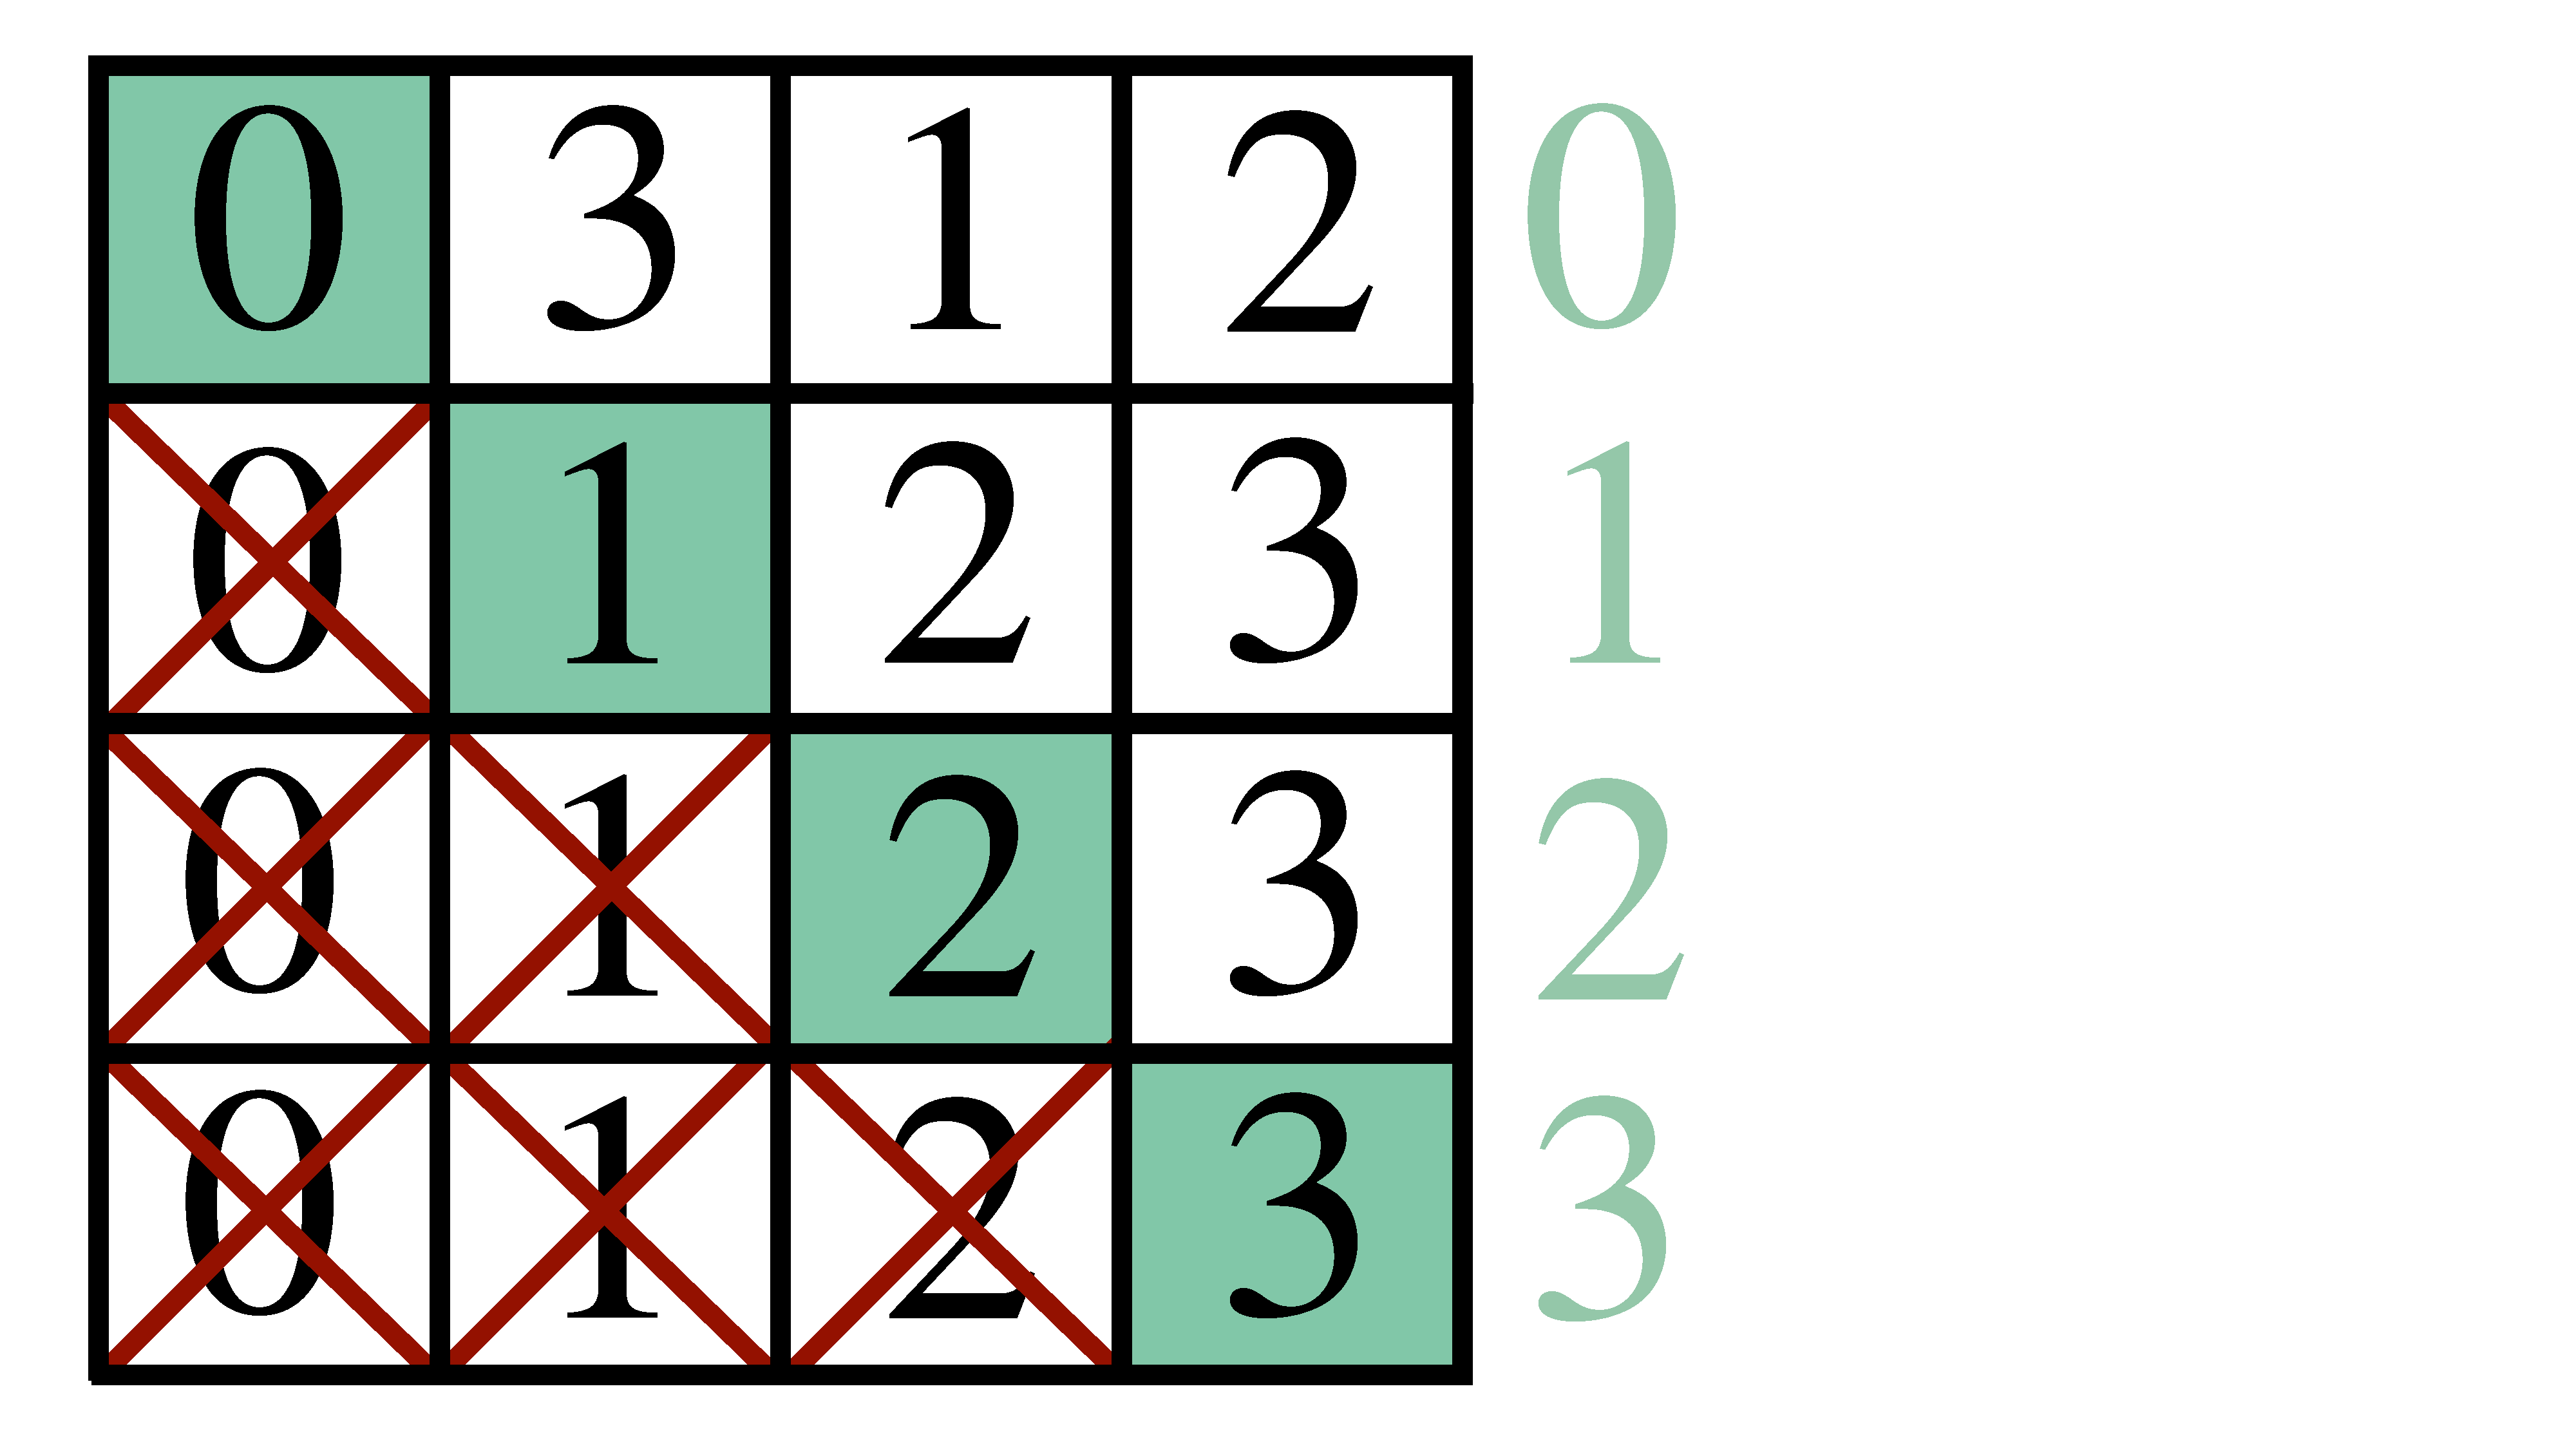
\includegraphics[width=\textwidth,trim=0mm 0mm 230mm 0mm, clip]{./figures/aMinRed4.pdf}
        \caption{Solution.}\label{sfig:aMinRed4}
    \end{subfigure} \hfill
    \caption{Reduction from \lfm to \am. \ref{sfig:aMinRed1} gives the \lfm instance and \ref{sfig:aMinRed2} its solution. \ref{sfig:aMinRed3} gives the \am instance from the reduction and \ref{sfig:aMinRed4} its solution.} \label{fig:aMinRed}
\end{figure}

Concluding, we use the \CC-hardness of \am to prove the \CC-hardness of \hac. 
\mainLowerPar*
% \begin{lemma}
% Average linkage HAC is \CC-complete, even on trees of diameter $6$.
% \end{lemma}

\begin{proof}
Our reduction shows how to reduce an instance of \am (\cref{l:am}) of size $n$ to an instance of average linkage HAC on a tree.
We build a rooted tree, in which each root-to-leaf path has length $2$ (i.e., the tree has depth $2$). %\rnote{(i.e., tree has depth $2$?)}\knote{Yes}.
We call the neighbors of the root \emph{internal} nodes.
Observe that each node is either the root, an internal node or a leaf.
The fact that the tree is rooted is only for the convenience of the description.
In the construction, we will begin by assigning each node an initial size (see the definition of \textit{size} in Section \ref{sec:prelims}) which is possibly larger than $1$ (but at most $\poly(n)$). We will later show how to remove these variable sizes, and reduce to the case where all nodes have initial size $1$ (as in the original definition of HAC).

The basic idea of our construction is as follows. Our HAC instance will consist of a rooted tree where each child of the root corresponds to a column of $A$ in our \am instance. HAC merges will then happen in phases where each phase corresponds to a row of $A$. In a given phase, exactly one internal node will merge with the root which will correspond to this internal node's column being minimum for the corresponding row of $A$. In order to guarantee this, each child of the root will have its own carefully selected children such that merging with these children guarantees the desired behavior in every phase. 
%\enote{Can somebody make sure this is correct?}

More formally, the tree is constructed as follows.
The root $r$ of the tree has initial size $n^8$.
It has $n$ children, each of initial size $n^4$---we denote them by $v_0, \ldots, v_{n-1}$.
The root is connected to its children using edges of weight $1$, i.e., $w(r,v_i) = 1$ for all $i=0,1,\dots,n-1$ (thus, the normalized weight of the edges $\{rv_i\}_{i=0}^{n-1}$ are each $\frac{1}{n^{12}}$ at the start).
Each internal node has $n(n+1)$ children (leaf nodes) grouped into $n$ groups of $n+1$ leaves each.  We write $C_{i,j} = \{v_{i,j,0}, v_{i,j,1}, \dots, v_{i,j,n}\}$ to denote the $j$-th group of children of the $i$-th internal vertex. 
All the leaves $v_{i,j,k}$ have initial size $1$. Thus, the vertices in the full graph in our construction consists of the root $r$, internal nodes $\{v_0,v_1,\dots,v_{n-1}\}$ and leaves $\cup_{i=0}^{n-1} \cup_{j=0}^{n-1} \cup_{k=0}^n \{v_{i,j,k}\}$

Let $r_i = n^8 + i \cdot n^4$ (for $0 \leq i < n$).
For each pair of an internal node and each of its groups there are only two distinct edge weights for edges between the internal node and the leaves in the group.
Specifically, for an internal node $v_j$ and group $C_{j,i}$ 
% \kgnote{Is this $C_{ij}$?} \rnote{I don't think so, since the index of the internal node is $j$. It is confusing because either we use $C_{j,i}$ or we have to have $A[j,i]$, since the internal node index corresponds to the columns of $A$.}\kgnote{I see, may be we can change the definition of $C_{ij}$ to $C_{ji}$ in the previous paragraph to keep it consistent and less confusing (also $v_{i,j,k}$)} 
of its children we have $A[i, j]+1$ edges of weight $\frac{1}{r_i - 1}$ and $n - A[i, j]$ edges of weight $\frac{1}{r_i + i \cdot n^3}$. Specifically, we set

\[ w(v_j, v_{j,i,k}) =\begin{cases} \frac{1}{r_i - 1} & \text{if } 0 \leq k \leq A[i,j] \\
\frac{1}{r_i + i \cdot n^3} & \text{if }  A[i,j] < k \leq n \\
\end{cases}\]



We call the two weights \emph{high-weight} and \emph{low-weight} edges, respectively. 
Note that their normalized weights are $\frac{1}{n^4(r_i - 1)}$ and $\frac{1}{n^4(r_i + i\cdot n^3)}$ respectively. Observe that the setting of \emph{high-weight} and \emph{low-weight} edges is independent of the internal node $v_j$, although the number of high versus low-weight edges depends on $A[i,j]$.
Moreover, note that even low-weight edges of any group $C_{j,i}$ have higher weights than high-weight edges of group $C_{j,i+1}$:
\begin{align*}
\frac{1}{n^4(r_i + i\cdot n^3)} & > \frac{1}{n^4(r_{i+1} + (i+1)\cdot n^3)} \iff \\
\frac{1}{n^8 + i \cdot n^4 + i\cdot n^3} & > \frac{1}{n^8 + (i+1)n^4 -1} \iff \\
i \cdot n^3 & < n^4 - 1.
\end{align*}
which follows from the fact that $i \leq n-1$.
%Note that the edge weights are hard-coded as functions of $A[i,j]$. Thus, it is clear that the reduction can be carried out in logspace (namely, the weight of each edge can be computed in log-space). 
%First, let us demonstrate that this reduction can be carried out in logspace.
%\knote{I'm not an expert, but it seems quite obvious, isn't it?}
We now demonstrate that the average linkage HAC on this instance works in $n$ phases numbered from $0$ to $n-1$, where in each phase $i$,
\begin{itemize}
\item $n-1$ internal nodes contract all of their incident group $i$ edges, and
\item one internal node contracts all of its high-weight edges to group $i$, after which it merges with the root.
\end{itemize}

Because of the internal node merging with the root, the root has incident leaves, but they are connected with edges of (normalized) edge weights $\leq \frac{1}{n^{15}}$ and so they will be irrelevant until all phases have been completed.
We  show that if we denote by $k_i$ the index of the internal node which merges with the root in phase $i$, the sequence $k_0, \ldots, k_{n-1}$ is a correct solution to the \am problem. 


%\hnote{We may want to add an illustration for the intermediate state corresponding to the following claim.}

In order to analyze the algorithm, we prove the following claim.
For convenience, let us define $w_i = n^4 + i \cdot (n+1)$. %\rnote{The internal nodes start with weight $n^4$, so surely $w_i$ should be larger than $n^4$? I think $n^3 \mapsto n^4$}\knote{Yeah, I changed $n^3$ to $n^4$ before and must have missed this.}

\begin{claim}
In the beginning of phase $i$, the graph is as follows:
\begin{enumerate}
    \item The size of the root node is $r_i+ i^2 \cdot \Delta_i$ for some $\Delta_i \in [0, n+1]$.\label{l:rootweight}
    \item Exactly $i$ internal nodes have been merged with the root, and the corresponding values $k_0, \ldots, k_{i-1}$ have been computed correctly.\label{l:correct}
    \item The size of each of the $n-i$ remaining internal nodes is $w_i$.\label{l:intweight}
    \item For all remaining internal nodes, \emph{all} leaves in groups $0, \ldots, i-1$ have been merged into their parents, and no leaves in groups $i, \ldots, n-1$ have been merged.\label{l:groups}
    \item The root may have incident leaves (resulting from internal nodes contracting into it) connected to the root with edges of normalized weights $\leq \frac{1}{n^{15}}$.\label{l:leaves}
\end{enumerate}
\end{claim}
\begin{proof}
We prove the above claim using induction on $i$.
The base case of $i=0$ follows directly from how the tree is constructed.

We now simulate a single phase.
The edges between the root and the internal nodes have (normalized) weights $\frac{1}{w_i(r_i + i^2 \cdot \Delta_i)} > \frac{1}{n^{15}}$.
Hence, the additional leaf nodes incident to the root (see \cref{l:leaves} of the Claim) are irrelevant.
Thus, the highest weight edge in the graph is surely incident to one of the internal nodes.
Observe that the relative order of edge weights between an internal node $v$ and its children does not change as the leaves are merged into $v$.
Therefore, given that groups $0, \ldots, i-1$ do not exist anymore, among edges between the internal nodes and leaves, the edges of group $i$ have the highest weights.
In the beginning of a phase the high-weight edges in that group have normalized weights $\frac{1}{w_i(r_i -1)}$ and the low-weight edges have weight $\frac{1}{w_i (r_i + i \cdot n^2)}$.

Hence, we have that if we sort the edges by their normalized weights, the top 3 classes of edges are, starting from the highest weight:
%\begin{enumerate}[label=(\textbf{\arabic*}), topsep=1pt,itemsep=2pt,parsep=pt,leftmargin=25pt]
\begin{enumerate}
    \item High-weight edges between internal nodes and leaves of group $i$.
    \item Edges between the root and the internal nodes.
    \item Low-weight edges between internal nodes and leaves of group $i$.
\end{enumerate}

\noindent We will show that the phase consists of the following sub-phases.
%\begin{enumerate}
\begin{enumerate}
\item First, there is some number of subphases, where each of $n-i$ internal nodes contract one incident high-weight edge.
\item Then, there is exactly one subphase, where $n-i-1$ nodes contract an incident high-weight edge and one internal node merges with the root.
\item Then, the remaining $n-i-1$ internal nodes merge with all of their group $i$ leaves (we do not analyze the order in this subphase, as it is irrelevant).
\end{enumerate}

Assume that each internal node has at least one high-weight edge in group $i$.
Then, the algorithm will execute a Type 1 subphase: the first $n-i$ steps of the algorithm would merge exactly one high-weight edge incident to each internal node.
Note that when an edge incident to an internal node $v$ merges, the weight of $v$ increases, and so the incident edge weights decrease.
This guarantees that in the considered $n-i$ steps exactly one merge per internal node happens.

Type 1 subphases of $n-i$ steps continue as long as each each internal node has at least one high-weight group $i$ edge in the beginning of the subphase.
Each Type 1 subphase also causes the weight of each internal node to increase by $1$.
Clearly, since nodes are being merged into internal nodes, the ordering of edge weights incident to any internal node does not change.

At some point, in the beginning of a subphase there is an internal node that does not have any incident high-weight edge in group $i$.
Assume that this happened after $p$ Type 1 subphases have completed.
Thus, the size of each internal node is $w_i + p$.
Since by the construction each internal node had a different number of high-weight edges in group $i$, there is exactly one node $v$ with no high-weight incident edges and that node merges with the root.
This is when Type 2 subphase happens.
First, $n-i-1$ internal nodes contract with a high-weight incident group $i$ edge.
At this point the edge weights are as follows.
The weight of an edge between $v$ and the root is $\frac{1}{(w_i+p)(r_i + i^2\cdot \Delta_i)}$ and the weight of a high-weight edge in group $i$ is
$\frac{1}{(w_i+p+1)(r_i-1)}$. We have that the former is larger since
\begin{align*}
(w_i+p)(r_i + i^2\cdot \Delta_i) & < (w_i+p+1)(r_i-1) \iff\\
(w_i+p)\cdot i^2\cdot \Delta_i & < r_i-1 \iff\\
(n^4 + i \cdot (n+1) + p) \cdot i^2 \cdot \Delta_i & < n^8 + i \cdot n^4 - 1 \Leftarrow \\
(n^4 + n \cdot (n+1) + n) \cdot n \cdot n^2 & < n^8 + i \cdot n^3 - 1.
\end{align*}
Thus, the internal node with no incident high-weight edges in group $i$ merges with the root.
Observe that this is exactly the internal node which had the lowest number of high-weight edges in group $i$ among all remaining internal nodes.
This immediately implies that $k_i$ is computed correctly, proving \cref{l:correct}.

We now show that in the remaining part of the phase the $n-i-1$ remaining internal nodes contract their incident group $i$ edges.
First, observe that the new size of the root node is
\[
r_i + w_i + p + i^2 \cdot \Delta_i = \left(n^8 + i \cdot n^4 + n^4\right) + \left(i \cdot (n+1) + i^2 \cdot \Delta_i + p\right) = r_{i+1} + (i+1)^2 \Delta_{i+1}
\]
for some $\Delta_{i+1} \in [0, n+1]$.
Note that we use the fact that both $\Delta_i$ and $p$ are upper bounded by $n+1$, which implies $i \cdot (n+1) + i^2 \cdot \Delta_i + p \leq (i+1)^2(n+1)$.
This proves \cref{l:rootweight}.
Thus for an internal node of weight $w$, the weight of its edge to the root is  
\[
\frac{1}{w \cdot (r_{i+1} + (i+1)^2 \Delta_{i+1})} \leq \frac{1}{w \cdot r_{i+1}} = \frac{1}{w \cdot (n^8 + (i+1) \cdot n^4)}.\]
On the other hand, its low-weight edges to group $i$ leaves have weight
\[
\frac{1}{w(n^8 + i(n^4 + n^2))}.
\]
As a result, in the remaining part of the current phase all internal nodes will contract all their incident group $i$ edges. This implies \cref{l:groups}.
Thus, the size of each internal node within the phase  increases to $w_i + (n+1) = n^4 + i \cdot (n+1) + n + 1 = n^4 + (i+1)(n+1)$, as required.
This proves \cref{l:intweight} and completes the proof.
\end{proof}


Finally, we now claim that, given an instance of \am with input index $x \in [0,n)$ and  an algorithm which can compute the solutions to Problem \ref{prob:hac}, we can compute the solution $k_x$ to Problem \ref{l:am} in logspace. To see this, note that it suffices to determine the value $k_x$ as defined above given an algorithm for \hac. To see this, note that for any internal node $i$, we can query the \hac algorithm to determine which time step $t_i$ it merged with the root. 
This does not directly tell us which phase $i$ merged with the root, but for a given $i$ we can determine if it merged in phase $x$ 
%\enote{phase $i$ or maybe for a given $x$?} 
by comparing $t_i$ with $t_j$ for all $j \in \{0,1,\dots,n-1\} \setminus \{i\}$, and checking if there are exactly $x-1$ values of $t_j$ smaller than $t_i$. This clearly can be verified in log-space. 
Repeating for all $i \in  \{0,1,\dots,n-1\}$ allows us to correctly determine the identity of the internal node that merged with the root in phase $x$, and therefore the value of $k_x$, in logspace as required.

To complete the proof of the Lemma it remains to show how to drop the assumption on the node sizes being initially not all equal to $1$.
In order to obtain a node of size $w$ it suffices to create a node of weight $1$ and initially connect it to $w-1$ auxiliary nodes using very high weight edges.
This will force the algorithm to merge all these auxiliary nodes and increase the size of that node to $w$.
Since the auxiliary leaves are connected only to the root and internal nodes (the leaves in our construction have weight $1$), the diameter of the tree does not increase.
\end{proof}


\section{Average Linkage HAC on Paths in \NC}\label{sec:pathupperbound}
In this section, we present an $\tilde{O}(n)$ work and $O(\mathsf{polylog}(n))$ depth algorithm for solving average linkage HAC on path graphs, provided that the aspect ratio of the input instance is bounded by $\poly(n)$.
%\kgnote{discuss/define aspect ratio earlier} 
%\hnote{Better exclude weight-zero edges in defn}
The {\em aspect ratio} is defined as $\mathcal{A} = W_{\max}/W_{\min}$, where $W_{\max} = \argmax_{e \in E} w(e)$ and $W_{\min} = \argmin_{e\in E} w(e)$ (note that this definition excludes all non-edges, which implicitly have a weight of 0).
The main algorithm for this section is presented in Algorithm~\ref{alg:paths}, which we first give a high-level overview of next, followed by a detailed description.


\begin{algorithm}[ht]
\caption{Average linkage HAC on paths; $\mathtt{ProcessChain}$ assumes that the input chain has a certain structure. However, this assumption can be removed easily (see \Cref{sec:pathupperbound})}\label{alg:paths}
\SetKwInput{Input}{Input}
% \KwIn{A path graph $G = (V, E, w)$}
\SetKwFunction{FHac}{PathHAC}
\SetKwFunction{Fchain}{ProcessChain}
\SetKwProg{Fn}{Function}{:}{}
\SetKwProg{parfor}{parallel for}{:}{}

\Input{A path graph $G = (V, E, w)$}
\Fn{\FHac{$x, y, w, S$}}{
Compute buckets $B_1,B_2,\ldots,B_T$ such that $B_i$ contains edges with weights in $((2/3)^{t}w_{\max}, (2/3)^{t-1}w_{\max}]$.\\
\For{$t=1$ to $T$}{
Let $\mathcal{C} \gets$ Nearest-neighbor chains on the induced graph $G[B_t]$.\\
\parfor{each $C \in \mathcal{C}$}{
\Fchain{$C$}
}
}
}
\BlankLine
\Input{A chain $C=(c_1,c_2,\ldots,c_N)$ such that $c_{i-1}$ is the nearest neighbor of $c_i$ and $(c_1,c_2)$ is a reciprocal pair.}
\Fn{\Fchain{$C,t$}}{
Split the chain $C$ at all indices $i$ such that $S(c_i) < 2S(c_{i-1})$, except $i=2$.\\
We get a set of contiguous \emph{subchains} $C_1,C_2,\ldots,C_K$. Subchain $C_j$ falls into one of two categories: 
(A) the nearest clusters in $C_{j-1}$ and $C_j$ merge, or 
(B) no two clusters from $C_{j-1}$ and $C_j$ merge.\\
Find the merge categories for all subchains to obtain the modified subchains $C_1',C_2',\ldots, C_K'$.\\
\parfor{each $j=1$ to $k$}{
Run average linkage HAC on $C_j'$ until no edge remains with weight within the threshold of $B_t$.
}

}
\end{algorithm}

In average linkage HAC, the weight (i.e., similarity) of edges monotonically decreases over time. 
Thus, our idea is to partition the edges into \emph{buckets} where the edges in any bucket have the same similarity, up to constant factors. 
Next, we process these buckets in {\em phases}, from the highest similarity bucket to the lowest. 
In each phase, we perform a modified version of the classic nearest-neighbor chain algorithm (\Cref{alg:nnchain}), wherein we compute the nearest-neighbor chains for the graph induced on the edges in that bucket, and process each chain independently. 
We note that when we use the terminology {\em nearest neighbor} of a vertex in what follows, we refer to the neighbor along the {\em highest weight edge} incident to the vertex.

Initially, each cluster is a singleton, and we might end up with $\Omega(n)$ sequential dependencies to resolve. 
However, we observe that in this special case when the size of every cluster is equal, starting with the reciprocal pair, every {\em alternate} edge in this chain can be merged independently, and the rest of the edges will be moved to a later bucket. 
We can compute the edges that will be merged easily via a simple $\mathsf{prefix\text{-}sum}$ routine~\cite{blellochscan}. 
However, when the cluster sizes are arbitrary, this observation no longer holds.
Nonetheless, we show that we can partition each chain further into $O(\log n)$-sized subchains such that, even though the dependencies within a subchain must be resolved sequentially, the dependencies across subchains can be resolved in parallel using a similar application of $\mathsf{prefix\text{-}sum}$. 
In this section we show (1) that our parallel algorithm is highly efficient (it runs near-linear time in the number of nodes) and runs in poly-logarithmic depth and (2) that our algorithm implies that the dendrogram height of a path input with polynomial aspect ratio is always poly-logarithmic.

%\section{Deferred Proofs from Section~\ref{sec:pathupperbound}}\label{apx:path}


\paragraph{Implementation Details and Correctness}
We now elaborate on certain implementation aspects of \Cref{alg:paths}. In \Cref{alg:paths}, there are two implicit assumptions made about the chains:
\begin{itemize}
    \item Every edge in $B_t$ is present in some chain in $\mathcal{C}$.
    \item Each chain can be represented as $(c_1,c_2,\ldots, c_N)$ such that $c_{i-1}$ is the nearest neighbor of cluster $c_i$, and $(c_1,c_2)$ is the \emph{reciprocal pair}. 
    Thus, the weights are in non-increasing order from left to right.
\end{itemize}
We will see later how to remove these assumptions. By the above assumptions, each chain will be a separate connected component in the graph induced on $B_i$, thus, allowing us to process each chain independently. In $\mathtt{ProcessChain}$, we split each chain at all indices such that $S(c_i) < 2 S(c_{i-1})$ giving us a set of subchains. This implies that for two adjacent clusters $c_{j-1},c_{j}$ in the same subchain, $S(c_j) \ge 2S_{j-1}$ (see \Cref{fig:path-subchains}). Thus, the size of a subchain cannot exceed $\log n$, and we can afford to process these subchains sequentially, while still obtaining low depth overall. 

\begin{figure}[ht]
    \centering
    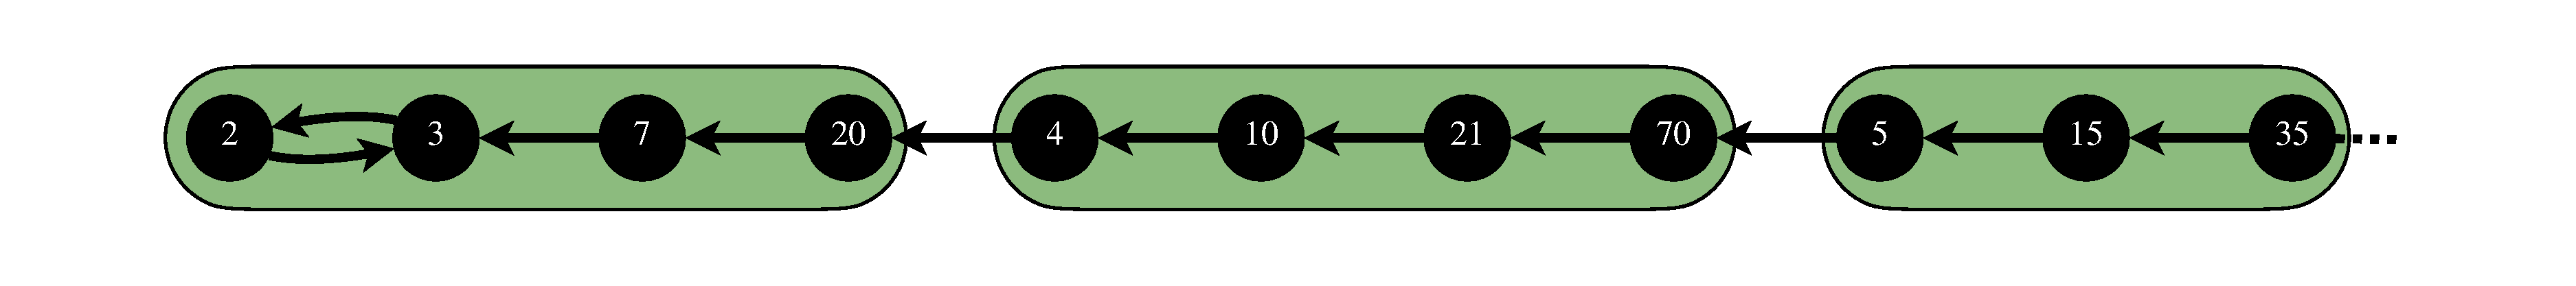
\includegraphics[width=0.9\textwidth]{figures/pathSubchains.pdf}
    \caption{An example describing the partition of a chain into subchains based on cluster sizes.}
    \label{fig:path-subchains}
\end{figure}

We now prove certain key properties about subchains. Let $u_0,u_1,u_2$ denote three contiguous clusters in a chain such that $u_0$ is the last cluster in its subchain, and $u_1$ is the first cluster of its subchain. $u_2$ may or may not belong to the same subchain as $u_1$.

\begin{lemma}\label{lem:path_A}
    If cluster $u_1$ first merges with the cluster (containing) $u_0$, then the weight of the edge $(u_1,u_2)$ reduces to at most $2/3$ times its previous weight.
\end{lemma}
\begin{proof}
    Let $x = w(e)/(S(u_1)S(u_2))$ denote the weight of edge $e=(u_1,u_2)$. If cluster $u_1$ merges with a cluster in its preceding subchain, the merged cluster will be of size at least $S(u_0)+S(u_1)$. Let $x'$ denote the new weight of edge $e$ after this merge. Then,
    \begin{align*}
        x' \le \frac{w(e)}{(S(u_0)+S(u_1))S(u_2)} \implies \frac{1}{x'} &\ge \frac{1}{x} + \frac{S(u_0)S(u_2)}{w(e)}\\
        \implies \frac{1}{x'} &\ge \frac{1}{x} + \frac{S(u_1)S(u_2)}{2w(e)}, & \text{since $S(u_0) \ge S(u_1)/2$}\\
        \implies \frac{1}{x'} &\ge \frac{3}{2x},
    \end{align*}
    Therefore, $x' \le 2x/3$.
\end{proof}

\begin{lemma}\label{lem:path_B}
    If cluster $u_1$ first merges with the cluster (containing) $u_2$, then the weight of the edge $(u_0,u_1)$ reduces to at most $1/3$ times its previous weight.
\end{lemma}
The proof follows by a similar argument as in \Cref{lem:path_A}. By \Cref{lem:path_A,lem:path_B}, each subchain falls into one of the following categories:
\begin{enumerate}[label=(\Alph*)]
    \item The first cluster of the subchain merges with a cluster in the preceding subchain (if exists).
    \item The first cluster of the subchain doesn't merge with a cluster from the preceding subchain.
\end{enumerate}
In either case, one of the edges incident on the first cluster of the subchain moves to a later bucket after it merges, disconnecting the two subchains in the induced graph. Thus, if a subchain falls into category (A), we can move its first cluster to the preceding subchain; if it falls into category (B), we make no changes. By this process, we obtained the modified subchains $C_1',C_2',\ldots,C_K'$, and by the above argument we can run average linkage HAC independently on them. Note that we do not run HAC to completion at these subchains, rather until we have edges with weight within the threshold defined by its bucket. 

Note that the first subchain of a chain will always fall into category (B) since it contains a reciprocal pair which is guaranteed to merge.
Running HAC on this subchain (starting with merging the reciprocal pair) determines whether the next subchain falls into the merge category (A) or (B), which in turn determines the merge category for the following subchain, and so on. 
We now show that we can propagate this merge behavior across subchains with the help of a simple prefix-sum routine in $\poly(\log n)$ depth.

\begin{lemma}\label{lem:path_prefix_sum}
    Given a chain of size $N$ partitioned into subchains $C_1,C_2,\ldots,C_K$, we can determine the merge category ((A) or (B)) for each subchain in $\tilde{O}(N)$ work and $\poly(\log n)$ depth.
\end{lemma}
\begin{proof}
    For subchain $C_j$, let $f(j,A)$ denote the resulting merge category of $C_{j+1}$ if $C_j$ belongs to category (A). Define $f(j,B)$ similarly. Firstly, recall that the category of $C_1$ is determined (it is always category (B)). 
    If $f(j,A) = f(j,B)$, for some $j$, this implies that the category of $C_{j+1}$ is determined regardless of the category of $C_j$. Thus, we can split the chain at subchain $C_{j+1}$ and deal with the two chains obtained, independently. We now assume that $f(j,A)\ne f(j,B)$ for all $j$.

    We create an array $A$ of size $K$ such that,
    \begin{align*}
        A[j] = \begin{cases}
            0 & \text{if $j=1$ and $f(1,B)=A$},\\
            1 & \text{if $j=1$ and $f(1,B)=B$},\\
            0 & \text{if $j>1$ and $f(j,A)=A$},\\
            1 & \text{if $j>1$ and $f(j,A)=B$}.
        \end{cases} 
    \end{align*}
    Let $B= \mathsf{prefix\text{-}sum}(A,\mathtt{XOR},0)$, i.e., $B[1]=0$ and $B[i]=A_1\oplus A_2 \oplus\ldots A_{i-1}$.
    In other words, we compute the prefix sum of the array $A$ with respect to the $\mathtt{XOR}$ function, using $0$ as the left identity element.
    % \lnote{What is $\bot$ here?}
%    \hnote{Shall we define this terminology? Wouldn't prefix ``sum'' be more widely understood?}
    Then, we claim that the merge category of subchain $C_j$ is (A) if $B[j]=0$, otherwise it is (B).

    To see this, consider subchains such that $f(j,A)=A$. These subchains propagate the same category (as them) to the next subchain, which can be viewed as an $\mathtt{XOR}$ operation with a $0$. Similarly, subchains that have $f(j,A)=B$ propagate the opposite category (as them) to the next subchain, which can be viewed as an $\mathtt{XOR}$ with $1$. $A[1]$ denotes the category of subchain $C_2$ that is determined by $C_1$. Thus, computing the $\mathsf{prefix\text{-}sum}$ correctly computes the categories for each subchain.

    The values of $f(j,A)$ (and $f(j,B)$) can be computed by simply simulating average linkage HAC sequentially at each subchain, assuming the category (A) (and (B)) at that subchain. 
    Since the subchain sizes are at most $\log n$, the work incurred to solve HAC on a subchain of size $r$ will be $O(r\log\log n)$.
    
    To see this, consider running Algorithm~\ref{alg:heapbased} on the chain, which we claim runs in $O(N\log\log n)$ work (and depth).
    This is because the heap-based algorithm for HAC (described in more detail in Section~\ref{sec:workupperbound}) on a path containing $r \leq \log n$ elements operates over a heap containing at most $\log n$ elements, and thus each of the at most $r$ merge operations require $O(\log \log n)$ time and only require updating the two neighboring edges incident to the merged edge.
    Since the algorithm used on each subchain is sequential, the depth at each subchain will also be $O(r\log\log n) \in O(\log n\log\log n)$. 
    The $\mathsf{prefix\text{-}sum}$ operation runs in $O(K)$ work and $O(\log K)$ depth. 
    
    Thus, the overall work for a chain containing $N$ elements will be $O(N\log\log n)$ and depth will be $O(\log n\log\log n)$.
\end{proof}

Since the edges are processed in non-increasing order of weight (due to bucketing), and \Cref{lem:path_A,lem:path_B,lem:path_prefix_sum} correctly computes the subchains and proves the correctness of processing these subchains independently, the overall correctness of the algorithm follows directly.

\paragraph{Work and Depth Bounds}
We will now argue the work and depth bounds of the overall algorithm.
Observe that, since the minimum possible weight is at least $W_{\min}/n^2$, the total number of phases will be $T \in O(\log \mathcal{A} + \log n) \in O(\log n)$. 
In each phase, we can compute the nearest neighbor chains in $O(n)$ work and $O(\log n)$ depth; the subchains can also be computed with similar work-depth bounds. By \Cref{lem:path_prefix_sum}, the total work incurred in finding the merge categories for each subchain and running average linkage HAC on these subchains, across all chains, in the worst case will be $O(n\log\log n)$ work and $O(\log n\log\log n)$ depth. Thus, the overall work of the algorithm is $O(n\log n\log\log n)$ and depth is $O(\log^2n\log\log n)$. 

Thus, we have the following theorem about the work and depth of the algorithm:
\mainUpperPar*

\paragraph{Resolving assumptions about chain structure}
\begin{figure}[ht]
    \centering
    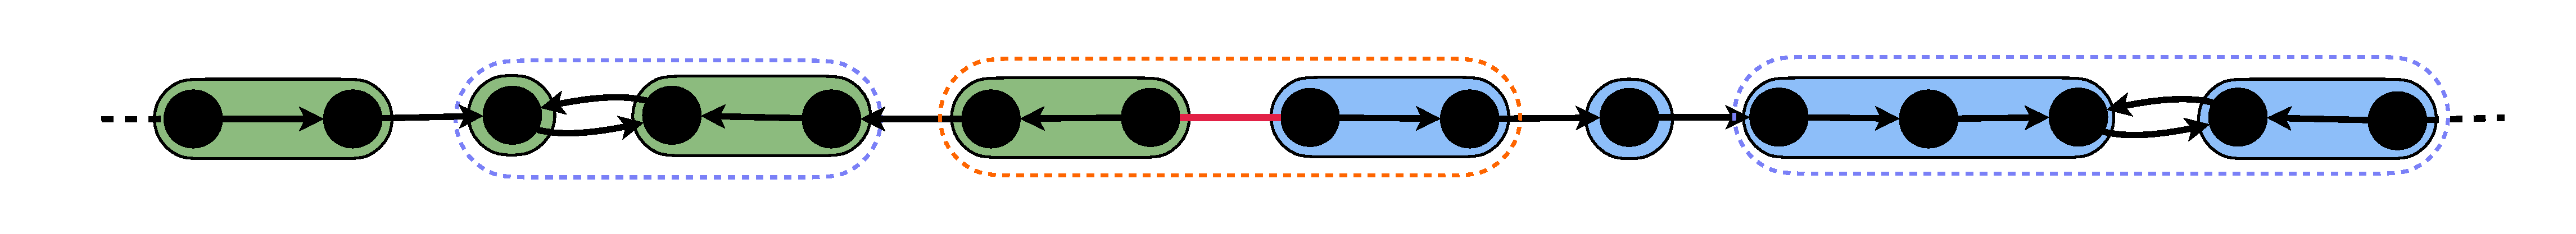
\includegraphics[width=\textwidth]{figures/pathGeneralChains.pdf}
    \caption{An example illustrating the general (possible) structure of the nearest neighbor chains computed in each phase of \Cref{alg:paths}. The red edge here is an example of an edge that is not present in any chain. The dotted lines represents the various subchain merges to address the assumptions made about the nearest neighbor chain structure in \Cref{alg:paths}.}
    \label{fig:path-general-chains}
\end{figure}
We will now address the assumptions made about the structure of chains in the algorithm. When the nearest neighbor chains are computed, the structure of the chains can be represented as 
$$(c'_{N'}\ldots, c_3',c_2', c_1',c_1,c_2,c_3,\ldots,c_{N}),$$
where $(c_1',c_1)$ is the reciprocal pair, $c'_{i-1}$ is the nearest neighbor of $c'_i$, and $c_{i-1}$ is the nearest neighbor of $c_i$. We can extend the idea of partitioning these chains into subchains as follows: partition the chains $(c_1,c_2, \ldots, c_N)$ and $(c'_1,c'_2,\ldots,c'_{N'})$, independently, into subchains using the same criterion as before. Now, merge the subchains containing $c_1$ and $c'_1$ resulting in a subchain of length at most $2\log n$ (see \Cref{fig:path-general-chains}). Then, independently propagate the merge behavior across these two sets of subchains, with the subchain containing $(c_1,c'_1)$ as the first subchain. 

Finally, when we compute the nearest neighbor chains, it is possible for some edges in the bucket to not be present in any chain. However, these edges can occur only between the last vertices of two chains (see \Cref{fig:path-general-chains}). Thus, after finding the merge categories for the subchains containing these vertices (in their respective chains), we can merge these two subchains along with the edge (whose size will be at most $4\log n$ in the worst case). It is not hard to extend the correctness and running time arguments when these modifications are incorporated.

\paragraph{Height of the dendrogram is \texorpdfstring{\boldmath$O(\log^2n)$}{O(log^2(n))}}
An interesting consequence of our algorithm is a constructive proof that the height of the dendrogram obtained when we run average linkage HAC on paths with polynomial aspect ratio is $O(\log^2n)$.



\begin{restatable}{theorem}{pathheight}\label{thm:pathheight}
    Average linkage HAC on path graphs with $\poly(n)$ aspect-ratio returns a dendrogram with height at most $O(\log^2n)$.
\end{restatable}

\begin{proof}
    Starting with phase 1, the algorithm runs average linkage HAC (partially) on independent $O(\log n)$-sized contiguous portions (i.e., subchains) of the path. Thus, each subchain will correspond to independent parts in the output dendrogram. Since there are $O(\log n)$ phases and the max-height generated in each phase is at most $O(\log n)$, we get an overall bound of $O(\log^2n)$ for the height in the worst case.
\end{proof}

% the algorithm partitions the edges into \emph{buckets} such that edges in each bucket have equal similarity, up to constant factors. Since the minimum possible similarity for an edge is at least $W_{\min}/n^2$, the number of buckets ($T$) will be in $O(\log \mathcal{A} + \log n) \in O(\log n)$ (due to bounded aspect ratio). Then, the algorithm runs in phases where in the $t$-th phase it computes the nearest neighbor chains in the induced graph $G[B_t]$. processes only edges from $B_t$, and computes the nearest neighbor chains


% \begin{itemize}
%     \item Partition the edges into buckets $B_1, B_2, \ldots, B_t$, where $B_i$ maintains edges with similarity in the range $((2/3)^{i}w_{\max}, (2/3)^{i-1}w_{\max}]$. Observe that, since the minimum possible similarity is at least $w_{\min}/n^2$, $t \in O(\log \mathcal{A} + \log n) \in O(\log n)$.
%     \item Run the following algorithm in $t$ phases. 
%     In the $i^{th}$ phase, the algorithm only considers edges in $B_i$ and pushes edges to later buckets as soon as their similarity drops below the threshold of $B_i$.
%     \begin{enumerate}
%         \item Compute the nearest neighbor chains. 
%         \hnote{We can add a pseudocode and some illustration to explain the algorithm here. We could also add an informal explanation first. Why NN chains are relevant and what subchains denote are not clear to the lay reader. The enumeration here is really not an algorithm, rather the description of the algorithm intertwined with notes about the proof. May be a good idea to decouple. I would avoid the bullet point style presentation in this section.}
%         We make the following two assumptions about these chains; we later show how to remove these assumptions.
%         \begin{itemize}
%           \item Each chain can be represented as $(v_1,v_2, v_3, \ldots, v_\ell)$ such that $v_{i-1}$ is the nearest neighbor of cluster $v_i$, and $(v_1,v_2)$ is the \emph{reciprocal pair}. Thus, the similarities are in non-increasing order from left to right.
%           \item Every edge in $B_i$ is present in some chain.
%         \end{itemize}
%         By these assumptions, each chain will be a separate connected component in the graph induced on $B_i$. Thus, we process each chain independently.
%         \item Fix some chain. Partition it further into a set of \emph{subchains}, where a subchain $(u_1, u_2, u_3, \ldots, u_s)$ is a \emph{contiguous} set of clusters such that $S(u_{i}) \ge 2S(u_{i-1})$. Observe that the size of a subchain cannot exceed $\log n$. Thus, we can afford to sequentially process each subchain. Additionally, we always include $v_1$ in the subchain containing $v_2$.
%         \item For a subchain $(u_1, u_2, u_3, \ldots, u_s)$, let $u_0$ denote the last vertex in the subchain preceding it in its chain (if exists). We have two ``merge categories'' here:
%         \begin{enumerate}[label = (\Alph*)]
%             \item $u_1$ first merges with some cluster in the preceding subchain: In this case, we will show that the similarity of edge $(u_1,u_2)$ reduces to at most $2/3$ times its previous similarity after this merge (see \Cref{lem:path_A}), thus pushing it to a later bucket.
%             \item $u_1$ first merges within its subchain: In this case, we will show that the similarity of edge $(u_0,u_1)$ reduces to at most $1/3$ times its previous similarity after this merge (see \Cref{lem:path_B}), thus pushing it to a later bucket.
%         \end{enumerate}
%         Thus, once we figure out the merge category for each subchain, we can run average-linkage HAC independently. Note that we do not run HAC to completion at these subchains, rather until we have edges with similarity within the threshold defined by $B_i$.
%         \item Note that the first subchain of a chain would always fall into category (B). Running HAC on this subchain (starting with merging the reciprocal pair) determines whether the next subchain falls into the merge category (A) or (B), which in turn determines the merge category for the following subchain, and so on. We can propagate this merge behavior across subchains with the help of a simple prefix-sum routine in $\tilde{O}(1)$ depth (see \Cref{lem:path_prefix_sum}).
%         \item Once the appropriate merge category ((A) or (B)) is determined at each subchain, run average-linkage HAC at each subchain, in parallel, until either all edges are merged or pushed to a later bucket.
%     \end{enumerate}
% \end{itemize}


% TODO:
% - If figured out, discuss how to extend this algorithm to trees, assuming oracle access to a CC-complete problem.


\begin{algorithm}[!t]\caption{\small The nearest-neighbor chain algorithm for HAC.}\label{alg:nnchain}
\KwIn{$G = (V, E, w)$}

\SetKwFunction{FNNChain}{NearestNeighborChain}
\SetKwProg{Fn}{Function}{:}{}

\Fn{\FNNChain{$G$}}{
$\clustering \gets$ clustering where each $v \in V$ is in a separate cluster and is {\em active}.\\
\For{each cluster $v \in V$}{
  \If {$v$ is active}{
    Initialize a stack $S$ initially containing only $v$ \\
    \While {$S$ is not empty}{
      $t \gets \textsc{Top}(S)$.\\
      $(t, b, w_{t,b}) \gets \textsc{BestEdge}(t)$.\label{line:nnchainbestedge} \\
      \If{$b$ is already on $S$}{
        $\textsc{Pop}(S)$. \\
        $\textsc{Merge}(t, \textsc{Top}(S))$.\label{line:nnchainmerge}  \ \  //\ {\em $t$ is marked as inactive; $\textsc{Top}(S)$ remains active.}\\
        $\textsc{Pop}(S)$.
       } \Else {
        $\textsc{Push}(S, b)$.
       }
    }
  }
}
}
\end{algorithm}

\section{\texorpdfstring{\boldmath$O(mh\log n)$}{O(mhlogn)} Upper Bound}\label{sec:workupperbound}

%\knote{I think we need to define 'active' clusters. Also, I think the pseudocodes never mark clusters as 'inactive'.}

In this section we show that we can solve graph-based average linkage HAC in $\tilde{O}(mh)$ time where $h$ is the {\em height} of the output dendrogram.
Thus, when $mh = o(n^{3/2})$ this algorithm improves over the lower bound from Section~\ref{sec:worklb}.
Interestingly, we give a simple analysis showing that either of the two classic approaches to HAC---the nearest-neighbor chain or heap-based algorithms---achieves this bound.
We give the pseudocode for the nearest-neighbor chain algorithm in Algorithm~\ref{alg:nnchain} and the heap-based algorithm in Algorithm~\ref{alg:heapbased}.
In a nutshell, in both algorithms initially all vertices start in their own cluster, and are {\emph{active}}.
As the algorithms proceed, they find edges to merge that the exact greedy HAC algorithm (Algorithm~\ref{alg:staticgraph}) will make and merge them, marking one of the endpoints as {\em inactive}.
This process continues until no further edges between active clusters remain.
We discuss the algorithms individually in more detail in what follows.

We start by discussing some data structures and details in how the algorithms carry out merges.

\paragraph{Neighborhood representation}
The neighbors of each vertex are stored in a max-heap supporting standard operations (e.g., \textsc{find-min}, \textsc{delete-min}, \textsc{insert}, \textsc{decrease-key}).
The priority of a neighbor is the average linkage weight of the edge to the neighbor.
At the start of the algorithm, the heaps are initialized with the initial neighbors of each vertex.
Let $N(A)$ represent the neighbors of a cluster $A$.
For concreteness in what follows, we use Fibonacci heaps~\cite{CLRS, fredman1987fibonacci}.


\paragraph{Merging clusters}
Next, we discuss how to implement the {\em merge} step in both algorithms, which merges two clusters $A$ and $B$, and their corresponding heaps (i.e., merging $N(A)$ and $N(B)$ and updating the average linkage weights of {\em all} edges affected by the merge).
We maintain the invariant that the heaps always store the correct average linkage weights of all edges.
We first compute $\mathcal{I}(A,B) = N(A) \cap N(B)$, which can be done by sorting both sets and merging the sorted arrays.
For each $C \in \mathcal{I}(A, B)$, without loss of generality, we remove the reference to $A$ in the heap and update the priority of $B$ to reflect the new average linkage weight from $C$ to $A \cup B$ using \textsc{decrease-key}.
Similarly, we update each $C \in N(A) \setminus \mathcal{I}(A, B)$ to reference $B$ instead of $A$.
Finally, for each $C \in N(A) \cup N(B)$ we update the priority of the edge $(C, B)$ to reflect the new size of $B$.

At the end of the merge: (1) $N(B)$ contains $N(A) \cup N(B) \setminus \{A, B\}$; (2) all edges in the updated $N(B)$ have their average linkage weight correctly set; and (3) after the update all $C \in N(B)$ no longer reference $A$, but point to $B$ and have their average linkage weights correctly set.
%\hnote{Shall we explicitly say that the two heaps are merged into one?}
%
The cost of this merge procedure is dominated by the cost of sorting $N(A)$ and $N(B)$; plugging in the cost bounds for any reasonable heap data structure (e.g., a Fibonacci heap) yields the following lemma:
\begin{lemma}\label{lem:merge}
Merging two clusters $A,B$ with $N(A) + N(B) = T$ can be done in $O(T \log n)$ time.
\end{lemma}


\paragraph{Nearest-Neighbor Chain Analysis}
As we run the nearest-neighbor chain algorithm (Algorithm~\ref{alg:nnchain}), the algorithm only requires two non-trivial operations beyond basic data structures (e.g., stacks and heaps):\footnote{In fact the same two primitives are also the only non-trivial ones used for the heap-based algorithm (Algorithm~\ref{alg:heapbased}) and thus we fully specify the details for this algorithm as well.}
%\knote{We need to add the algorithm pseudocode for NN chain here}:
\begin{enumerate}
  \item \textsc{BestEdge}($C$): fetch the highest similarity edge incident to a cluster $C$.
  \item \textsc{Merge}($A, B$): merge the clusters $A,B$ into a cluster $A \cup B$ (represented, without loss of generality by $B$). Thus after the merge, $A$ is inactive, and $B$ remains active.
%  \knote{I think this means that $A$ becomes inactive, not, as we say in pseudocodes, one of A, B, right?}
\end{enumerate}

Using the data structures above, we can implement both operations very quickly. 
In particular, Lemma~\ref{lem:merge} gives the time for merging two clusters, and \textsc{BestEdge}($C$) can be implemented in $O(1)$ time using the \textsc{find-min} operation.

After merging two clusters that are reciprocal ``best'' neighbors, the algorithm back-tracks to the third vertex in the chain and restarts the process, using calls to \textsc{BestEdge}.
The cost of these calls can be charged to the merges, resulting in a total of $O(n)$ time for the $n-1$ merges.
The time that still must be accounted for is that of \textsc{Merge}.

\begin{claim}\label{claim:mergecost}
The total amount time spent to perform all merges made by the nearest-neighbor chain algorithm is $O(mh\log n)$.
\end{claim}
\begin{proof}
Split each edge $(u,v)$ into two directed edges $(u,v)$ and $(v,u)$, since the edge will be present initially in both $N(u)$ and $N(v)$ (and the intermediary clusters they form until they are merged).

Consider a directed edge $(u,v)$, and the merges it experiences as it flows along the path from the initial cluster containing it ($u$) to the cluster where it is finally merged.
The dendrogram that the algorithm constructs has height $h$ by definition, and thus the length of this path is at most $h$.
In each node on the path, the edge contributes a cost of $O(\log n)$ to the merge cost in Lemma~\ref{lem:merge}.
Thus, the cost of this edge across the entire path is at most $O(h \log n)$.

Applying this charging argument for all $2m$ directed edges, the total cost over all merges is $O(mh\log n)$.
\end{proof}


Putting together the above yields the following theorem.
\mainUpperSec*


\begin{algorithm}[!t]\caption{The heap-based algorithm for HAC.}\label{alg:heapbased}
\KwIn{$G = (V, E, w)$}

\SetKwFunction{FHeapBased}{HeapBasedHAC}
\SetKwProg{Fn}{Function}{:}{}

\Fn{\FHeapBased{$G$}}{
$\clustering \gets$ clustering where each $v \in V$ is in a separate cluster and is {\em active}.\\
Let $H$ be a max-heap storing the highest-weight edge incident to each active cluster in the graph \\
\While{$|H| > 1$}{
  Let $e=(u, v, w_{u,v})$ be the max weight edge in $H$. \\
  Delete $e$ from $H$. \\
  \If {$v$ is inactive} { \label{line:heapbadextract}
    Let $e' = (u, v', w_{u,v'}) = \bestedge{u}$. \\
    Insert $e'$ into $H$. \label{line:heapinsertfirst} \\
  } \Else {
    $x = \textsc{Merge}(u, v)$.    \ \  //\ {\em $u$ is marked as inactive; $v$ remains active.} \\
    Let $e' = (x, y, w_{x,y}) = \bestedge{x}$. \\
    Insert $e'$ into $H$. \\
  }
}
}
\end{algorithm}
\paragraph{Heap-Based Algorithm}

We note it is easy to extend the argument above to obtain a similar bound for the heap-based algorithm 
(pseudocode shown in Algorithm~\ref{alg:heapbased}).
In particular, beyond the cost for merging, which is the same in the nearest-neighbor chain algorithm and the heap-based algorithm (captured by Claim~\ref{claim:mergecost}), the only extra work incurred by the heap-based algorithm is due to edges unsuccessfully extracted from the heap (Line~\ref{line:heapbadextract} of Algorithm~\ref{alg:heapbased}). 
The number of such unsuccessful edges is at most $m$, and each such edge incurs $O(\log n)$ work due to an extra call to \bestedge{u}, for a total of $O(m\log n)$ extra work.
Thus the total work of the heap-based algorithm is also $O(mh\log n)$.

\begin{theorem}
There is an implementation of the heap-based algorithm for average linkage HAC that runs in $O(mh \log n)$ time where $h$ is the height of the output dendrogram.
\end{theorem}


%\knote{Technically, Alg 1 does not use a heap.}





\section{Conclusion}
In this paper, we studied the parallel and sequential complexity of hierarchical
graph clustering. We gave new classic and fine-grained reductions for Hierarchical Agglomerative Clustering (HAC) under the average linkage
measure that likely rule out efficient algorithms for {\em exact} average linkage, parallel or otherwise. 
We also showed that such impossibility results can be circumvented if the output dendrogram has low height or is a path. An interesting question is whether such structure can be leveraged for other variants of interest of average linkage HAC: for example, can we can obtain dynamic algorithms for HAC that are also parameterized by the height?

\newpage
\begin{thebibliography}{10}

\bibitem{abboudhac}
Amir Abboud, Vincent Cohen-Addad, and Hussein Houdrouge.
\newblock {\em Subquadratic high-dimensional hierarchical clustering}.
\newblock 2019.

\bibitem{abboud2024faster}
Amir Abboud, Nick Fischer, and Yarin Shechter.
\newblock Faster combinatorial k-clique algorithms.
\newblock {\em arXiv preprint arXiv:2401.13502}, 2024.

\bibitem{alman2021refined}
Josh Alman and Virginia~Vassilevska Williams.
\newblock A refined laser method and faster matrix multiplication.
\newblock In {\em Annual ACM-SIAM Symposium on Discrete Algorithms (SODA)}, pages 522--539. SIAM, 2021.

\bibitem{ABP01}
N.~S. Arora, R.~D. Blumofe, and C.~G. Plaxton.
\newblock Thread scheduling for multiprogrammed multiprocessors.
\newblock {\em ACM Transactions on Computer Systems}, 34(2), Apr 2001.

\bibitem{affinity}
MohammadHossein Bateni, Soheil Behnezhad, Mahsa Derakhshan, MohammadTaghi Hajiaghayi, Raimondas Kiveris, Silvio Lattanzi, and Vahab Mirrokni.
\newblock Affinity clustering: Hierarchical clustering at scale.
\newblock In {\em Annual Conference on Neural Information Processing Systems (NeurIPS)}, pages 6864--6874, 2017.

\bibitem{benzecri}
J-P Benz{\'e}cri.
\newblock Construction d'une classification ascendante hi{\'e}rarchique par la recherche en cha{\^\i}ne des voisins r{\'e}ciproques.
\newblock {\em Cahiers de l'analyse des donn{\'e}es}, 7(2):209--218, 1982.

\bibitem{blellochscan}
Guy~E Blelloch.
\newblock Scans as primitive parallel operations.
\newblock {\em IEEE Transactions on computers}, 38(11):1526--1538, 1989.

\bibitem{blelloch2020optimal}
Guy~E. Blelloch, Jeremy~T. Fineman, Yan Gu, and Yihan Sun.
\newblock Optimal parallel algorithms in the binary-forking model.
\newblock In {\em {ACM} Symposium on Parallelism in Algorithms and Architectures (SPAA)}, 2020.

\bibitem{BL98}
Robert~D. Blumofe and Charles~E. Leiserson.
\newblock Space-efficient scheduling of multithreaded computations.
\newblock 27(1), 1998.

\bibitem{boly2012hierarchical}
M{\'e}lanie Boly, Vincent Perlbarg, Guillaume Marrelec, Manuel Schabus, Steven Laureys, Julien Doyon, M{\'e}lanie P{\'e}l{\'e}grini-Issac, Pierre Maquet, and Habib Benali.
\newblock Hierarchical clustering of brain activity during human nonrapid eye movement sleep.
\newblock {\em Proceedings of the National Academy of Sciences}, 109(15):5856--5861, 2012.

\bibitem{hac-reward}
Vincent Cohen-Addad, Varun Kanade, Frederik {Mallmann-Trenn}, and Claire Mathieu.
\newblock Hierarchical clustering: Objective functions and algorithms.
\newblock {\em Journal of the ACM (JACM)}, 66(4), 2019.

\bibitem{cook2014complexity}
Stephen~A Cook, Yuval Filmus, and Dai Tri~Man Le.
\newblock The complexity of the comparator circuit value problem.
\newblock {\em ACM Transactions on Computation Theory (TOCT)}, 6(4):1--44, 2014.

\bibitem{coppersmith1982asymptotic}
Don Coppersmith and Shmuel Winograd.
\newblock On the asymptotic complexity of matrix multiplication.
\newblock {\em SIAM Journal on Computing}, 11(3):472--492, 1982.

\bibitem{CLRS}
Thomas~H. Cormen, Charles~E. Leiserson, Ronald~L. Rivest, and Clifford Stein.
\newblock {\em Introduction to Algorithms (3rd edition)}.
\newblock MIT Press, 2009.

\bibitem{dhulipala2021hierarchical}
Laxman Dhulipala, David Eisenstat, Jakub Lacki, Vahab Mirrokni, and Jessica Shi.
\newblock Hierarchical agglomerative graph clustering in nearly-linear time.
\newblock In {\em International Conference on Machine Learning (ICML)}, pages 2676--2686, 2021.

\bibitem{dhulipala2022hierarchical}
Laxman Dhulipala, David Eisenstat, Jakub Lacki, Vahab Mirrokni, and Jessica Shi.
\newblock Hierarchical agglomerative graph clustering in poly-logarithmic depth.
\newblock {\em Annual Conference on Neural Information Processing Systems (NeurIPS)}, 35:22925--22940, 2022.

\bibitem{dhulipala2023terahac}
Laxman Dhulipala, Jakub {\L}{\k{a}}cki, Jason Lee, and Vahab Mirrokni.
\newblock Terahac: Hierarchical agglomerative clustering of trillion-edge graphs.
\newblock {\em Proceedings of the ACM on Management of Data}, 1(3):1--27, 2023.

\bibitem{eisen1998cluster}
Michael~B Eisen, Paul~T Spellman, Patrick~O Brown, and David Botstein.
\newblock Cluster analysis and display of genome-wide expression patterns.
\newblock {\em Proceedings of the National Academy of Sciences}, 95(25):14863--14868, 1998.

\bibitem{fredman1987fibonacci}
Michael~L Fredman and Robert~Endre Tarjan.
\newblock Fibonacci heaps and their uses in improved network optimization algorithms.
\newblock {\em Journal of the ACM (JACM)}, 34(3):596--615, 1987.

\bibitem{greenlaw2008parallel}
Raymond Greenlaw and Sanpawat Kantabutra.
\newblock On the parallel complexity of hierarchical clustering and cc-complete problems.
\newblock {\em Complexity}, 14(2):18--28, 2008.

\bibitem{hua2017mgupgma}
Guan-Jie Hua, Che-Lun Hung, Chun-Yuan Lin, Fu-Che Wu, Yu-Wei Chan, and Chuan~Yi Tang.
\newblock {MGUPGMA}: a fast {UPGMA} algorithm with multiple graphics processing units using {NCCL}.
\newblock {\em Evolutionary Bioinformatics}, 13:1176934317734220, 2017.

\bibitem{juan}
J~Juan.
\newblock Programme de classification hi{\'e}rarchique par l'algorithme de la recherche en cha{\^\i}ne des voisins r{\'e}ciproques.
\newblock {\em Cahiers de l'analyse des donn{\'e}es}, 7(2):219--225, 1982.

\bibitem{king1967step}
Benjamin King.
\newblock Step-wise clustering procedures.
\newblock {\em Journal of the American Statistical Association}, 62(317):86--101, 1967.

\bibitem{kobren2017hierarchical}
Ari Kobren, Nicholas Monath, Akshay Krishnamurthy, and Andrew McCallum.
\newblock A hierarchical algorithm for extreme clustering.
\newblock In {\em International Conference on Knowledge Discovery and Data Mining (KDD)}, pages 255--264, 2017.

\bibitem{lance1967general}
Godfrey~N Lance and William~Thomas Williams.
\newblock A general theory of classificatory sorting strategies: 1. hierarchical systems.
\newblock {\em The computer journal}, 9(4):373--380, 1967.

\bibitem{lau2021algorithms}
Joshua Lau and Angus Ritossa.
\newblock Algorithms and hardness for multidimensional range updates and queries.
\newblock In {\em Innovations in Theoretical Computer Science Conference (ITCS)}, 2021.

\bibitem{le2012faster}
Fran{\c{c}}ois Le~Gall.
\newblock Faster algorithms for rectangular matrix multiplication.
\newblock In {\em Symposium on Foundations of Computer Science (FOCS)}, pages 514--523. IEEE, 2012.

\bibitem{irbook}
Christopher~D Manning, Prabhakar Raghavan, and Hinrich Sch{\"u}tze.
\newblock {\em Introduction to Information Retrieval}.
\newblock Cambridge University Press, 2008.

\bibitem{mayr1992complexity}
Ernst~W Mayr and Ashok Subramanian.
\newblock The complexity of circuit value and network stability.
\newblock {\em Journal of Computer and System Sciences}, 44(2):302--323, 1992.

\bibitem{monath2021scalable}
Nicholas Monath, Kumar~Avinava Dubey, Guru Guruganesh, Manzil Zaheer, Amr Ahmed, Andrew McCallum, Gokhan Mergen, Marc Najork, Mert Terzihan, Bryon Tjanaka, et~al.
\newblock Scalable hierarchical agglomerative clustering.
\newblock In {\em International Conference on Knowledge Discovery and Data Mining (KDD)}, pages 1245--1255, 2021.

\bibitem{moseley-wang}
Benjamin Moseley and Joshua~R. Wang.
\newblock Approximation bounds for hierarchical clustering: Average linkage, bisecting k-means, and local search.
\newblock In {\em Annual Conference on Neural Information Processing Systems (NeurIPS)}, pages 3094--3103, 2017.

\bibitem{moseley2023approximation}
Benjamin Moseley and Joshua~R Wang.
\newblock Approximation bounds for hierarchical clustering: Average linkage, bisecting k-means, and local search.
\newblock {\em Journal of Machine Learning Research}, 24(1):1--36, 2023.

\bibitem{mllner2011modern}
Daniel M{\"u}llner.
\newblock Modern hierarchical, agglomerative clustering algorithms.
\newblock {\em arXiv preprint arXiv:1109.2378}, 2011.

\bibitem{murtagh2012algorithms}
Fionn Murtagh and Pedro Contreras.
\newblock Algorithms for hierarchical clustering: an overview.
\newblock {\em Wiley Interdisciplinary Reviews: Data Mining and Knowledge Discovery}, 2(1):86--97, 2012.

\bibitem{murtagh2017algorithms}
Fionn Murtagh and Pedro Contreras.
\newblock Algorithms for hierarchical clustering: an overview, ii.
\newblock {\em Wiley Interdisciplinary Reviews: Data Mining and Knowledge Discovery}, 7(6):e1219, 2017.

\bibitem{pedregosa2011scikit}
Fabian Pedregosa, Ga{\"e}l Varoquaux, Alexandre Gramfort, Vincent Michel, Bertrand Thirion, Olivier Grisel, Mathieu Blondel, Peter Prettenhofer, Ron Weiss, Vincent Dubourg, et~al.
\newblock Scikit-learn: Machine learning in python.
\newblock {\em the Journal of machine Learning research}, 12:2825--2830, 2011.

\bibitem{shearer1985alglib}
JM~Shearer and Michael~A Wolfe.
\newblock Alglib, a simple symbol-manipulation package.
\newblock {\em Communications of the ACM}, 28(8):820--825, 1985.

\bibitem{sneath1973principles}
Peter Henry~Andrews Sneath.
\newblock The principles and practice of numerical classification.
\newblock {\em Numerical taxonomy}, 573, 1973.

\bibitem{subramanian1989new}
Ashok Subramanian.
\newblock {\em A new approach to stable matching problems}.
\newblock Stanford University, 1989.

\bibitem{tsenghac}
Tom Tseng, Laxman Dhulipala, and Julian Shun.
\newblock Parallel batch-dynamic minimum spanning forest and the efficiency of dynamic agglomerative graph clustering.
\newblock In {\em ACM Symposium on Parallelism in Algorithms and Architectures (SPAA)}, page 233–245, 2022.

\bibitem{virtanen2020scipy}
Pauli Virtanen, Ralf Gommers, Travis~E Oliphant, Matt Haberland, Tyler Reddy, David Cournapeau, Evgeni Burovski, Pearu Peterson, Warren Weckesser, Jonathan Bright, et~al.
\newblock Scipy 1.0: fundamental algorithms for scientific computing in python.
\newblock {\em Nature methods}, 17(3):261--272, 2020.

\bibitem{williams2012multiplying}
Virginia~Vassilevska Williams.
\newblock Multiplying matrices faster than coppersmith-winograd.
\newblock In {\em Annual ACM Symposium on Theory of Computing (STOC)}, pages 887--898, 2012.

\bibitem{williams2010subcubic}
Virginia~Vassilevska Williams and Ryan Williams.
\newblock Subcubic equivalences between path, matrix and triangle problems.
\newblock In {\em Symposium on Foundations of Computer Science (FOCS)}, pages 645--654, 2010.

\bibitem{williams2024new}
Virginia~Vassilevska Williams, Yinzhan Xu, Zixuan Xu, and Renfei Zhou.
\newblock New bounds for matrix multiplication: from alpha to omega.
\newblock In {\em Annual ACM-SIAM Symposium on Discrete Algorithms (SODA)}, pages 3792--3835. SIAM, 2024.

\bibitem{zhao2002evaluation}
Ying Zhao and George Karypis.
\newblock Evaluation of hierarchical clustering algorithms for document datasets.
\newblock In {\em Conference on Information and Knowledge Management (CIKM)}, pages 515--524, 2002.

\end{thebibliography}


%\newpage
%\begin{appendix}
%\section{Average Linkage HAC on Trees is \texorpdfstring{\CC}{CC}-Complete}
In this section, we show that Average Linkage HAC on trees is in \CC, and hence, combined with the \CC-Hardness result, proves that it is \CC-Complete. In particular, we show that Average Linkage HAC on trees can be (log-space) reduced to a polynomial-many instances of a generalization of Adaptive Minimum, which we also show is \CC-Complete. We first recall a more general matching problem that is known to be \CC-Complete.

\begin{problem}[\lfbm]\label{dfn:LFBMM} An instance of lexicographically first maximal b-matching (LFM B-Matching) consists of a graph $G=(V, E)$ with vertices ordered as $V = (v_0, v_1, \ldots, v_{n-1})$. Further, for each vertex $v$ we are given a number $b(v)$. The lexicographically first maximal b-matching is the matching obtained by running the greedy algorithm for maximal matching on edges ordered first by their lower endpoint and then their higher endpoint such that the number of edges in the matching incident on any vertex $v$ doesn't exceed $b(v)$. That is, in this ordering $e = \{v_i, v_j\}$, with $i<j$, precedes $e' = \{v_{i'}, v_{j'}\}$, with $i'<j'$, iff (1) $i < i'$ or (2) $i = i'$ and $j < j'$. If any ties persist, i.e. multi-edges exist, break them arbitrarily. Our goal is to decide if a designated input edge is in the LFM B-Matching.
\end{problem}
In the case of multi-edges, any copy being in the matching is sufficient. Alternatively, we can also have a pre-defined ordering on the copies and break ties according to this ordering. 

\begin{theorem}\label{thm:LFBMCCComplete}
    \lfbm is \CC-Complete.
\end{theorem}
The proof follows by a standard reduction of B-Matching to Matching, and the fact that LFM Matching on general graphs is \CC-Complete~\cite{mayr1992complexity}.

\begin{problem}[\amj]\label{l:amj}
    An instance of \amj consists of a ($0$-based indexed) $n \times n$ matrix $A$ where each cell consists of two values: weight ($A[i,j].\weight$), and jump ($A[i,j].\jump$). For each row, the weights form a permutation of $\{0, \ldots, n-1\}$, whereas the jump values lie in the range $[0,n)$. We are also given some index $x \in [0, n)$. The goal is to simulate the following algorithm.
    Start with $I = \{0, \ldots, n-1\}$ and $i=0$, execute the following steps while $i \le x$:
    \begin{enumerate}
        \item Let $k_i = \argmin_{j \in I} A[i, j].\weight$.
        \item Set $I := I \setminus \{k_i\}$.
        \item For each $\ell=i+1$ to $i+A[i,k_i].\jump$, set $k_\ell = \Null$.
        \item Set $i = i + A[i, k_i].\jump$.
    \end{enumerate}
    Our goal is to compute $k_x$.
\end{problem}

\begin{lemma}
    \amj is \CC-Complete.
\end{lemma}
\begin{proof}
    Observe that \am is a special case of \amj when all the jump values are $1$. Thus, \amj is also \CC-Hard. We now prove that it is in \CC by reducing it to the \lfbm problem. 
    
    For each row $i \in [0,n)$ we introduce a node $r_i$. For each pair $(i,j) \in [0,n)\times[0,n)$, we introduce a column node $c_{i,j}$ and a corresponding auxiliary node $a_{i,j}$. Let $k$ be a parameter whose value will be determined later. We set the capacities $b(r_i) = b(c_{i,j}) = b(a_{i,j}) = k/{(i+1)^2}$. Next, we introduce 4 types of edges: 
    \begin{enumerate}[label=(\roman*)]
        \item Between nodes $r_i$ and $c_{i,j}$, introduce $k/(i+1)^2$ edges.
        \item Between nodes $c_{i,j}$ and $a_{i,j}$, introduce $k/(i+1)^2$ edges.
        \item Between nodes $a_{i,j}$ and $c_{i+1,j}$, introduce $k/(i+2)^2$ edges.
        \item Let $t = A[i,j].\jump$. If $t>0$, for each $\ell=1$ to $t-1$, introduce $k/(i+\ell+1)^2$ edges between nodes $a_{i,j}$ and $r_{i+\ell}$.
    \end{enumerate}
    Finally, we define the ordering on the vertices. For row $i$, the first node in the ordering will be $r_i$, followed by the column nodes $c_{i,j}$, for $j\in [0,n)$, ordered by their weights in $A[i,j]$. Next, the $n$ auxiliary nodes $a_{i,j}$ follow, again ordered by their corresponding weights in $A[i,j]$. The ordering of row $i+1$ is placed after the ordering of row $i$, thus obtaining the overall ordering on nodes.

    Intuitively, the auxiliary node acts as a switch that is triggered when its corresponding column node doesn't match with it, i.e. the column node matches with the row node. When it is triggered, it blocks all future column nodes from participating in matches with row nodes via a ``chain-reaction''. It also matches and saturates the capacities of all row nodes that get skipped due to the jump value at that cell, thus simulating a jump.

    We claim that $k_i = j$ iff $r_i$ is matched to $c_{i,j}$ ($b(r_i)$ times), and $k_i = \Null$ iff $r_i$ is matched to $a_{i',k_{i'}}$ for some $i'<i$ ($b(r_i)$ times). We prove this by induction on $i$. Consider the index $i$. Let $i'$ denote the previous index that was matched to a column node $c_{i',j'}$. Let $t = A[i',j'].\jump$. By induction, we know that $k_{i'}=j'$, and $k_{s} = \Null$ for all $s \in [i'+1,i-1]$ implying that $t \ge i-i'-1$. If $t \ge i-i'$, then observe that $k_i=\Null$. Here, 



\end{proof}

\begin{theorem}\label{thm:avgtreeCCComplete}
    Average linkage HAC on trees is \CC-Complete.
\end{theorem}
\begin{proof}
    By \Cref{thm:mainLowerPar}, we know that it is \CC-hard. We now prove it is in \CC. We follow a similar framework used by \Cref{alg:paths} for the Paths case. Bucket the edges by weights and process them one-by-one. Consider the subgraph obtained by the graph induced on the edges in the current bucket. If its a forest with multiple connected components, we can process each component independently. So, we can assume that we have a tree. Root the tree at the largest vertex by size. Now, we decompose the tree into \emph{blocks} as follows: If the size of a vertex is at most $1/2$ the size of its parent, then include it in its parent's block. Otherwise, start a new block at that vertex. Observe that each vertex belongs to exactly one block, and since the cluster sizes reduces by a constant factor as we go down, the height of the subtree induced on any block will be at most $\log n$. If we contract each block into a single vertex, we get a tree representation of this block decomposition. Note that the structure of this tree can be arbitrary. For simplifying the presentation, we start with the assumption that we have only one block. We remove these assumptions gradually.

    Consider the case when the block has height $2$, i.e., we have a star graph rooted at the center. How do we process a star? Since these edges share an endpoint, they will be merged sequentially. Further, they will be merged in the sorted order of their initial weights since only the common endpoint's size is changing, and thus, the relative ordering of these edges will be preserved.

    Now, consider a block of height $3$. Here, we have a root, its children whom we call internal nodes, and their children whom we call leaves.
    % The subtree rooted at an internal node behaves similar to the star case discussed above, except that sometimes the internal node will prefer to merge with the root. If the root prefers that child at the same time, we can merge them and the remaining leaves in that subtree can be dropped as the edges from the root to these leaves will have its weight dropped by a constant factor after this merge.

    Now we will consider a path of blocks rooted at one of the end blocks. Look at one of the inter-block edges $(u,v)$. If $(u,v)$ decides to merge with the block of $u$, then the weight of every edge incident to $v$ in the block of $v$ drops by a constant factor (similar to the cases obtained in \Cref{alg:paths}). Thus, starting with the first block, we can propagate the merging behavior of these inter-block edges in a similar manner as in \Cref{lem:path_prefix_sum} using a prefix-sum routine. 

    Finally, we return to the original arbitrary tree structure on the blocks. Given this, we compute a heavy-light decomposition (solvable in NC) on the tree structure. We start by applying the path algorithm discussed above to the leaf-paths.

\end{proof}
%
%\end{appendix}


\end{document}
